\documentclass[11pt,a4paper,oneside]{book}
\usepackage[T1]{fontenc}
\usepackage{fontspec}
\IfFontExistsTF{Spectral}{\setmainfont{Spectral}[Ligatures=TeX]}{\setmainfont{TeX Gyre Pagella}}
\IfFontExistsTF{Spectral}{\newfontfamily\headingfont{Spectral}}{\newfontfamily\headingfont{TeX Gyre Pagella}}
\usepackage[a4paper,top=2.2cm,bottom=2.2cm,left=2.4cm,right=2.4cm]{geometry}
\usepackage{graphicx}
\usepackage{xcolor}
\usepackage{colortbl}
\usepackage{tabularx}
\usepackage{booktabs}
\usepackage{titlesec}
\usepackage{tcolorbox}
\usepackage{fancyhdr}
\usepackage[hidelinks]{hyperref}
\usepackage{enumitem}

\definecolor{crimson}{HTML}{C1121F}
\definecolor{ink}{HTML}{111113}
\definecolor{lightgrey}{HTML}{F1F1F2}
\definecolor{midgrey}{HTML}{5C5C61}

\color{ink}
\renewcommand{\familydefault}{\rmdefault}

\titleformat{\part}[display]
  {\headingfont\bfseries\Huge\color{crimson}\centering}
  {\partname\ \thepart}{12pt}{\Huge\color{ink}}
\titleformat{\chapter}[display]
  {\headingfont\bfseries\color{ink}}
  {\filleft\Large\color{crimson}\chaptertitlename\ \thechapter}{14pt}{\Huge}
\titlespacing*{\chapter}{0pt}{10pt}{24pt}
\titleformat{\section}{\headingfont\bfseries\Large\color{ink}}{\thesection}{0.8em}{}
\titleformat{\subsection}{\headingfont\bfseries\large\color{ink}}{\thesubsection}{0.8em}{}

\newtcolorbox{notebox}{
  colback=lightgrey, colframe=crimson, boxrule=0pt,
  leftrule=2.4pt, arc=0pt, left=8pt, right=8pt, top=6pt, bottom=6pt,
  fontupper=\small
}

\pagestyle{fancy}
\fancyhf{}
\fancyhead[L]{\small\color{midgrey}\nouppercase{\leftmark}}
\fancyhead[R]{\small\color{midgrey}LoveLaundry --- System Manual}
\fancyfoot[C]{\small\color{midgrey}\thepage}
\renewcommand{\headrulewidth}{0.3pt}

\setlength{\parindent}{0pt}
\setlength{\parskip}{6pt}
\linespread{1.18}

\begin{document}

\begin{titlepage}
\centering
\vspace*{0.6cm}


\includegraphics[width=0.62\linewidth]{images/cover.png}\par
\vspace{1.2cm}
{\headingfont\Large\color{crimson}LOVE LAUNDRY}\par
\vspace{0.4cm}
{\headingfont\Huge System Manual}\par
\vspace{0.5cm}
{\itshape\large Laundry, Shop, Hotel and Linen Room Operations}\par
\vfill
{\large Rasindu Dulshan Siriwardhana}\par
\vspace{0.3cm}
{\small\itshape BSc. (Hons) Engineering (Computer Engineering) --- Second Class Upper Division\\
Faculty of Engineering, University of Ruhuna}\par
\vspace{0.6cm}
{\footnotesize\color{midgrey} FIRST EDITION \(\cdot\) OCTOBER 2026}
\end{titlepage}

\frontmatter
\tableofcontents
\mainmatter
Copyright and document controlLoveLaundry — System Manual

\textsc{\small\color{crimson}Copyright and document control}\par\medskip
\chapter{Document Control}
\subsection*{Copyright}
Copyright © 2026 Rasindu Dulshan Siriwardhana. All rights reserved. This manual and the LoveLaundry platform it describes are proprietary works. No part of this document may be reproduced, stored in a retrieval system, transmitted in any form or by any means — electronic, mechanical, photocopying, recording or otherwise — or disclosed to any third party without the prior written consent of the copyright holder, except as expressly permitted in the Licence on the following page.

\subsection*{Identification}
\begin{center}\small
\begin{tabularx}{\linewidth}{|X|X|}
\hline
Document title & LoveLaundry — System Manual \\ \hline
Document identifier & LL-SM-001 \\ \hline
Version & 1.0 — first complete issue \\ \hline
Issue date & 24 October 2026 \\ \hline
Status & Issued for operational use \\ \hline
Classification & Internal — Proprietary \\ \hline
Document owner & Rasindu Dulshan Siriwardhana, Developer and Systems Architect \\ \hline
Applies to & LoveLaundry platform release 1.x — six FastAPI services and four React front ends \\ \hline
Review cycle & Reviewed at each minor release and after every Severity 1 incident \\ \hline
Retention & Retained for the life of the platform plus seven years \\ \hline
Total pages & 105, including cover and appendices \\ \hline
\end{tabularx}
\end{center}
Copyright and document controlLoveLaundry — System Manual

\textsc{\small\color{crimson}Copyright and document control · continued}\par\medskip
LicenceLoveLaundry — System Manual

\textsc{\small\color{crimson}Licence}\par\medskip
\textsc{\small\color{crimson}Legal}\par\medskip
\chapter{Proprietary Software Licence}
Terms governing use of the LoveLaundry platform and of this manual.

\textbf{Copyright © 2026 Rasindu Dulshan Siriwardhana. All Rights Reserved.}

The LoveLaundry platform — its services, front ends, schemas, deployment configuration — is proprietary software, licensed and not sold. No ownership or intellectual-property right is transferred; all rights remain with the copyright holder.

\subsection*{1. Permitted use}
\begin{itemize}
\item The copyright holder, and any person expressly authorised in writing, may install, run, configure and maintain the platform for the operation of LoveLaundry laundry, shop, hotel-desk and linen-room services, and may keep one copy of this manual per licensed deployment.
\item Hotel client users may use the Hotel Desk application to view only the gate passes, deliveries, invoices and statements belonging to their own  within the laundry that issued their account.\texttt{client\_name}
\end{itemize}
\subsection*{2. Restricted use}
\begin{itemize}
\item No copying, redistribution, sublicensing, resale, publication or public display of the software or this manual, in whole or in part, without prior written consent.
\item No reverse engineering, decompilation or derivation of source code or database structure, except where such restriction is prohibited by law, and no removal of copyright, licence or attribution notices.
\item No access to the data of a tenant other than the one granted, and no attempt to bypass tenant scoping, authentication or authorisation controls.
\end{itemize}
\subsection*{3. Confidentiality, warranty, liability and term}
LicenceLoveLaundry — System Manual

\textsc{\small\color{crimson}Licence · continued}\par\medskip
ContentsLoveLaundry — System Manual

ContentsLoveLaundry — System Manual

ContentsLoveLaundry — System Manual

List of FiguresLoveLaundry — System Manual

\section*{List of Figures}
List of TablesLoveLaundry — System Manual

\section*{List of Tables}
\part{Foundation}
\textsc{\small\color{crimson}Part One · Introduction}\par\medskip
\chapter{Introduction}
\begin{quote}\itshape What LoveLaundry is, the operation it was built for, and the vocabulary its users already speak.\end{quote}
\section{1.1 Purpose}
This manual documents the LoveLaundry platform: a multi-tenant operations system for a commercial laundry that also serves a retail shop counter, hotel clients, and its own linen room. It exists so that the people who run, support and extend the platform have one authoritative description of how it is put together and how it is used — not a marketing overview, and not a substitute for reading the code, but the document that makes the code and the operation legible to each other.

The manual serves three audiences at once. Operators — counter staff, supervisors, linen-room attendants, hotel front-office users — need precise, numbered procedures and a clear statement of what the system will and will not let them do. Administrators need to know how tenants, users, memberships and hotel client accounts are created, and what the security model enforces on their behalf. Engineers and support staff need the architecture, the failure modes, the recovery paths and the measured state of the test suites, so that an incident can be diagnosed without rediscovering the design under pressure.

Every statement in this manual is either derived from the implementation as it stands or is explicitly marked as a target, a policy or a recommendation. Where the platform does not yet do something, the manual says so. Chapter 12 in particular reports measured test results rather than aspirational ones, and names the gaps — no browser-driven end-to-end suite, no load testing — instead of implying coverage that does not exist.

\section{1.2 Scope}
1 · IntroductionLoveLaundry — System Manual

The manual covers the platform as deployed for a single laundry business operating four front ends against a shared service estate. The boundary is set out below so that readers know when they have left the documented surface.

\begin{center}\small
\begin{tabularx}{\linewidth}{|X|X|X|}
\hline
\rowcolor{lightgrey}
\textbf{Area} & \textbf{Documented here} & \textbf{Boundary note} \\ \hline
Gate passes and deliveries & Yes — full & Creation, editing, status, dispatch and the linen lines attached to each pass. \\ \hline
Bills and payments & Yes — full & Bill generation from deliveries, payment recording, balances and day close totals. \\ \hline
Shop counter sales & Yes — full & Counter bills, quick bill, shift totals. Stock valuation is outside the platform. \\ \hline
Hotel client portal & Yes — full & Read-only operational and financial view scoped to one .\texttt{client\_name} \\ \hline
Linen room & Yes — full & Tag lifecycle, scanning, inventory and discrepancy handling. \\ \hline
Infrastructure & Partial & Topology, backup and recovery are documented; provider-specific console steps are not. \\ \hline
\end{tabularx}
\end{center}
\section{1.3 Who the system serves}
LoveLaundry is one platform with four working surfaces. Each exists because a different group of people does a different job and at a different speed. The design keeps them on one dataset while giving each a purpose-built interface.

The laundry businessThe core operation: collecting soiled linen and garments by gate pass, washing and finishing them, delivering them back, and billing for the work. The laundry app (quotations-ui) is the full-surface application — gate passes, deliveries, bills, quotations, workers, reports, the monthly matrix, dispatch and day close. It is where supervisors and managers spend their day.

1 · IntroductionLoveLaundry — System Manual

The shop counterA retail and walk-in service point. Customers arrive with a bag, not an account. The Shop Counter app is deliberately narrow: a today view, a bill list, a quick bill pad and a day close.

Hotel clientsHotels are the laundry's largest customers and its most demanding readers of records. A hotel is a separate entity in the platform: it is the carried on gate passes, deliveries, bills and quotations. Hotel staff sign in with a client account and see only their own property's records — never another hotel's, and never the laundry's internal costs.notclient\_name

The linen roomThe linen room is where physical items are counted, tagged, washed and reconciled. The Linen Room app turns that physical work into a digital trail: each tag is scanned at every stage, from collection through wash, press and readiness to delivery, with explicit actions for items that go missing, arrive damaged or are retired from service. Its users work one-handed with a scanner, so the interface is a single scan field and a short list of valid next actions.

\section{1.4 Design principles}
Seven principles explain most of the decisions in the codebase. They are stated here because they are also the grounds on which a change should be rejected.

\begin{center}\small
\begin{tabularx}{\linewidth}{|X|X|}
\hline
\rowcolor{lightgrey}
\textbf{Principle} & \textbf{What it means in practice} \\ \hline
Tenant from the token & The  is read from verified JWT claims. No request parameter, header or body field can set or override it. Missing context fails closed rather than falling back to an unscoped query.\texttt{laundry\_id} \\ \hline
One operation, one record & Gate passes, deliveries and bills are separate documents with explicit links, so each can be corrected without rewriting history. A bill is derived from deliveries; it does not absorb them. \\ \hline
Money is additive and reversible & Payments are records, not field mutations. Balances are computed. Corrections are new records that reference the original, so an audit trail survives every mistake. \\ \hline
Physical truth is scanned & The linen lifecycle advances only through explicit scan actions. No status is inferred from time passing, and no bulk update silently skips a stage. \\ \hline
Interfaces match the job & Counter staff get speed; linen staff get one scan field; hotels get read-only clarity; managers get the full surface. No single screen tries to serve all four. \\ \hline
Degrade, do not disappear & When a dependency is unavailable the affected feature stops and says so, while independent features continue. Chapter 11 states exactly what remains usable. \\ \hline
Recoverable by design & Backups, point-in-time recovery and restore drills are part of the product, not an afterthought. Chapter 10 defines the targets and the procedure. \\ \hline
\end{tabularx}
\end{center}
1 · IntroductionLoveLaundry — System Manual

\begin{notebox}WarningAny change that resolves a tenant from a request body or header is a security defect, not a feature — as is any change that lets a hotel client token reach a staff endpoint.\end{notebox}
\section{1.5 Glossary of domain terms}
The platform uses the vocabulary of the laundry trade. These terms recur throughout the manual and in the interface, and they do not always mean what a software reader would expect.

\begin{center}\small
\begin{tabularx}{\linewidth}{|X|X|}
\hline
\rowcolor{lightgrey}
\textbf{Term} & \textbf{Meaning in LoveLaundry} \\ \hline
Gate pass & The document that accompanies goods leaving or entering the premises. It records the client, the date, the item lines and quantities, and it is the origin of every downstream delivery and bill. A gate pass is the unit of operational truth: if it is not on a pass, it did not happen. \\ \hline
Delivery & The act and record of returning finished goods to the client. A delivery references the gate pass lines it fulfils, carries the delivered quantities, and is the input to billing. Partial deliveries against one pass are normal. \\ \hline
Bill & A financial document raised for one client over a period or a set of deliveries. It states quantities, rates, charges, discounts and tax, and it holds the balance outstanding. A bill is not edited once paid; corrections are made by credit or adjustment records. \\ \hline
Linen tag & A physical label with a unique identifier attached to an item or bundle. The tag is the join between the physical item and its digital record; scanning it advances the lifecycle. Tags are printed from the Linen Room app and retired when an item leaves service. \\ \hline
Day close & The end-of-day reconciliation. It freezes the day's totals — bills raised, payments received, shop sales, deliveries — and marks the business date closed so that later edits cannot silently change reported figures. Each front end has its own close, and the laundry close is the authoritative one. \\ \hline
Monthly matrix & A grid of clients against days of the month showing daily quantities and values, used to reconcile contract volumes and to spot missing or duplicated entries. It is a reporting artefact, generated from gate passes and deliveries, not a separately maintained ledger. \\ \hline
Quotation & A priced offer to a prospective or existing client, with line items, rates and validity. A quotation can be converted into operational work but does not itself create a bill. \\ \hline
Shop bill & A counter sale to a walk-in customer, recorded in the shop-app rather than the laundry ledger. Shop bills carry their own numbering and are reconciled at shop day close. \\ \hline
Dispatch & The release of finished goods to the delivery route. Dispatch records who released what, to which vehicle or driver, and at what time, closing the loop between the linen room and the client. \\ \hline
Return & Goods coming back from a client — rejected items, unused linen, or items sent in error. A return references the original delivery where one exists. \\ \hline
Client account & A login belonging to a hotel client organisation, stored in the  collection of user-service. It carries a  of one laundry and one ; it is not a membership and grants no staff capability.\texttt{client\_accounts}\texttt{client\_scope}\texttt{client\_name} \\ \hline
Tenant / laundry & The laundry business that owns a set of records. Represented by . Every business document carries it and every query filters on it.\texttt{laundry\_id} \\ \hline
Membership & The link between a user and a laundry, carrying the user's role in that laundry. A user may hold memberships in more than one laundry; each session acts in exactly one. \\ \hline
Capability & A named permission such as  or . Roles are bundles of capabilities; endpoints check capabilities, not role names.\texttt{bill:write}\texttt{linen:scan} \\ \hline
Discrepancy & A mismatch between expected and scanned linen quantities or statuses. Discrepancies are recorded, not corrected silently, so that loss patterns remain visible. \\ \hline
\end{tabularx}
\end{center}
1 · IntroductionLoveLaundry — System Manual

\begin{notebox}Note on “hotel”Throughout this manual, “hotel” refers to a client organisation identified by the  string. It is never a database entity, never a tenant, and never a login domain of its own. Chapter 2.8 explains why this matters for isolation.\texttt{client\_name}\end{notebox}
\textsc{\small\color{crimson}Part One · System Overview and Architecture}\par\medskip
\chapter{System Overview and Architecture}
\begin{quote}\itshape Six services, four front ends, three databases, one tenancy rule.\end{quote}
\section{2.1 Service map}
LoveLaundry is a service-oriented system built from Python/FastAPI services, each owning a bounded part of the business, behind four React front ends. There is no shared application server and no shared in-process state: a front end calls a service over HTTPS with a bearer token, and the service answers from the database it owns. Figure 1 shows the estate as deployed.

2 · System Overview and ArchitectureLoveLaundry — System Manual

\begin{figure}[htbp]
\centering
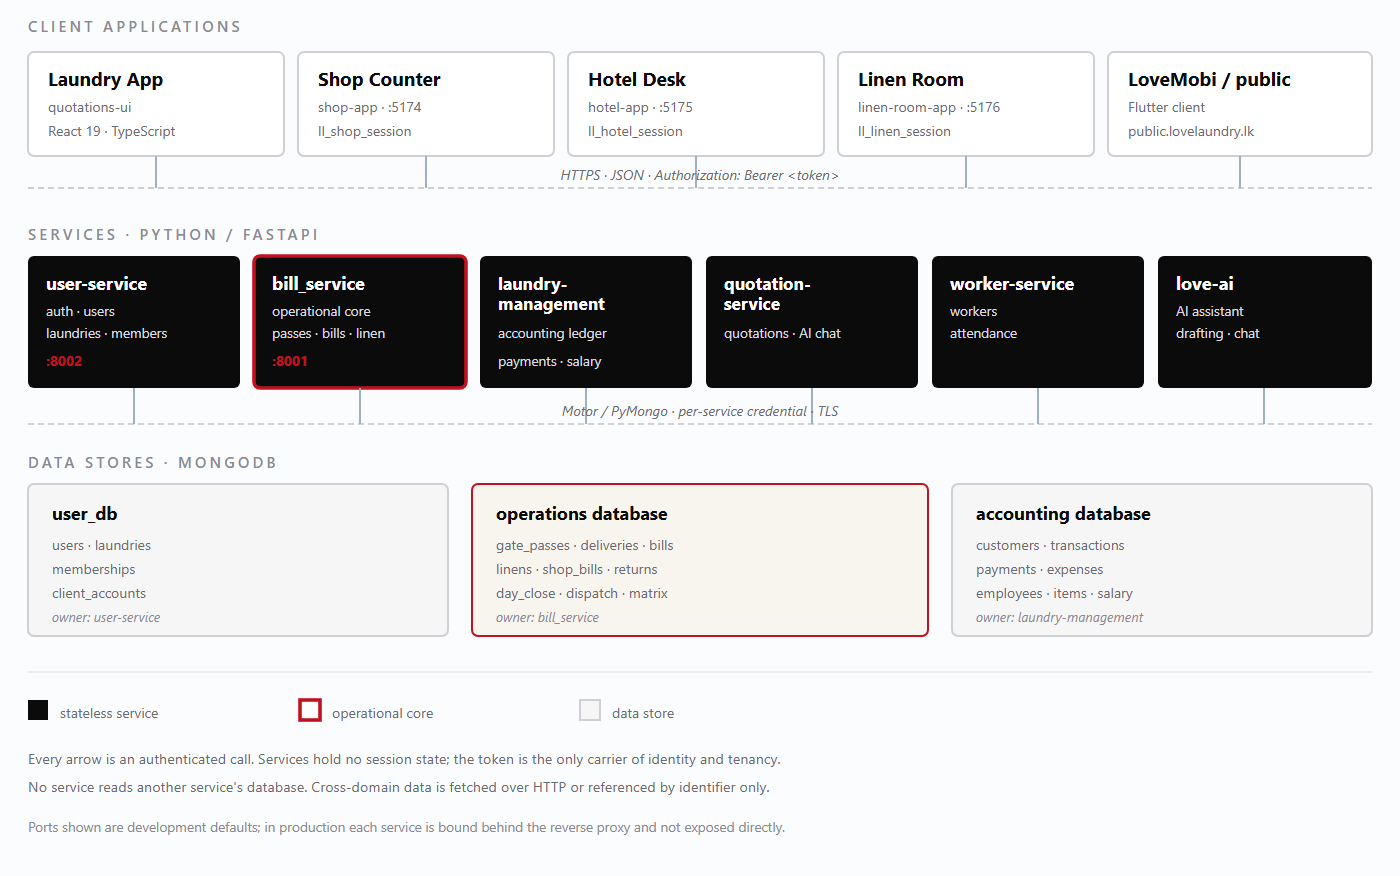
\includegraphics[width=\linewidth]{images/fig-01.png}
\caption{— Service map. Five client applications call six FastAPI services; three MongoDB databases hold identity, operations and accounting data respectively. The operational core, bill\_service, is outlined in the accent colour.Figure 1}
\end{figure}
\begin{notebox}Why this shapeThe split follows ownership, not technology. Identity and tenancy change rarely and must be trusted by everyone, so they live in user-service. Operational documents change constantly and are read by all four front ends, so they live in bill\_service. Accounting follows its own reporting calendar and retention rules, so it is isolated in laundry-management.\end{notebox}
\section{2.2 Service catalogue}
Each service is independently deployable and owns its collections. The table below is the authoritative list of services, their responsibilities and their development ports.

2 · System Overview and ArchitectureLoveLaundry — System Manual

\begin{center}\small
\begin{tabularx}{\linewidth}{|X|X|X|X|}
\hline
\rowcolor{lightgrey}
\textbf{Service} & \textbf{Port} & \textbf{Responsibility} & \textbf{Owns} \\ \hline
user-service & 8002 & Authentication for staff and hotel clients, user records, laundries (tenants), memberships, hotel client accounts, role and capability resolution, token issuance. & , , , \texttt{users}\texttt{laundries}\texttt{memberships}\texttt{client\_accounts} \\ \hline
bill\_service & 8001 & The operational core: gate passes, deliveries, bills, shop bills, linens and tag lifecycles, returns, monthly matrix, dispatch, day close and dashboards. & Operational collections in the operations database \\ \hline
laundry-management & — & Accounting: customers, transactions, payments, expenses, salary, employees and priced items. Feeds financial reporting and the payment ledger. & Accounting database \\ \hline
quotation-service & — & Quotation drafting, pricing line items and the AI chat surface used to assemble offers. & Quotation collections \\ \hline
worker-service & — & Worker records, assignment and attendance. Supplies worker lists to the laundry app. & Worker collections \\ \hline
love-ai & — & AI assistance: drafting, summarisation and conversational help over permitted data. Invoked by the other services and by the laundry app. & No business data of record \\ \hline
\end{tabularx}
\end{center}
\subsection*{Division of responsibility}
is the only issuer of tokens and the only authority on who a caller is. It answers three questions for every other service: is this token genuine, which laundry is this session acting in, and what may this caller do. It stores the membership snapshot that is copied into the token, so downstream services do not need a database lookup to resolve tenancy.\textbf{user-service}

is where the business actually happens. Gate passes are created here, linen lines are attached here, deliveries are recorded here, and bills are raised here. It is also the service the shop counter and hotel desk call, and the one that must remain available for the business to trade.\textbf{bill\_service}

holds the money in its accounting form: customers, transactions, payments, expenses, salaries, employees and items. It is separate from the operational ledger because accounting records have different retention, correction rules and audience. A payment recorded operationally is mirrored into accounting, never edited in place in either system.\textbf{laundry-management}

owns the pre-sale conversation. A quotation is a priced proposal with line items and validity; it can become work, but it never becomes a bill by itself.  owns people and attendance.  holds no data of record: it reads through the services that do, and anything it drafts must be saved through a normal write path with a normal capability check.\textbf{quotation-service}\textbf{worker-service}\textbf{love-ai}

\subsection*{Ports and addressing}
The ports above are development defaults. In a deployed environment the reverse proxy terminates TLS and routes by path prefix, and the services listen on the loopback interface only. A service port is never published to the internet, and no front end hard-codes one: service base URLs are supplied at build time through Vite environment variables.

2 · System Overview and ArchitectureLoveLaundry — System Manual

\begin{center}\small
\begin{tabularx}{\linewidth}{|X|X|X|X|}
\hline
\rowcolor{lightgrey}
\textbf{Caller} & \textbf{Callee} & \textbf{Purpose} & \textbf{Failure mode} \\ \hline
All services & user-service & Token verification and capability resolution & Fail closed \\ \hline
shop-app, hotel-app, linen-room-app & bill\_service & Operational reads and writes & Surface unavailable \\ \hline
bill\_service & laundry-management & Mirror payment and customer records & Queue and retry \\ \hline
\end{tabularx}
\end{center}
\begin{notebox}WarningService-to-service calls are authenticated with the calling user's token, not with a privileged backdoor credential. If the user could not perform the action directly, the platform does not perform it on their behalf through an internal call.\end{notebox}
\section{2.3 Front-end applications}
Four React applications share a toolchain and a design language but not a codebase. Each is built with React 19, TypeScript, Vite 8 and Tailwind CSS 4, and each is deployed as static assets behind the same reverse proxy. Two additional surfaces — the guest-billing print view and the public marketing site — are served alongside them.

\begin{center}\small
\begin{tabularx}{\linewidth}{|X|X|X|X|X|}
\hline
\rowcolor{lightgrey}
\textbf{Application} & \textbf{Dev port} & \textbf{Sign-in} & \textbf{Session key} & \textbf{Primary audience} \\ \hline
quotations-ui \\ Laundry app & 5173 & Staff sign-in; existing application, extended for the new modules & — & Owners, managers, supervisors, office staff \\ \hline
shop-app \\ Shop counter & 5174 & against user-service\texttt{POST /auth/login} & ll\_shop\_session & Counter staff and shop supervisors \\ \hline
hotel-app \\ Hotel desk & 5175 & against user-service\texttt{POST /client/auth/login} & ll\_hotel\_session & Hotel front-office and housekeeping managers \\ \hline
linen-room-app \\ Linen room & 5176 & Staff sign-in with linen-room roles & ll\_linen\_session & Linen supervisors and housekeepers \\ \hline
public.lovelaundry.lk & — & None — public marketing site & — & Prospective clients \\ \hline
LoveMobi & — & Staff sign-in (Flutter client) & — & Owners and managers on the move \\ \hline
\end{tabularx}
\end{center}
\subsection*{Shared conventions}
2 · System Overview and ArchitectureLoveLaundry — System Manual

\begin{itemize}
\item Each application stores its token under its own key — , ,  — so that two applications open in the same browser cannot overwrite each other's session, and so that a token issued to one audience is never silently reused by another.\textbf{Session storage.}\texttt{ll\_shop\_session}\texttt{ll\_hotel\_session}\texttt{ll\_linen\_session}
\item Every request attaches . No application puts a token in a query string, and none stores a token in a cookie readable by scripting.\textbf{Token in the header.}\texttt{Authorization: Bearer <token>}
\item Buttons are hidden when a capability is absent, but the check that matters is on the server. Hiding a control is a usability measure, not a security control.\textbf{No client-side authorisation.}
\item When a call fails with 401 the application clears its session and returns to sign-in; when it fails with 403 it shows a permission message and leaves the session intact; when it fails with 5xx it shows a retry affordance and does not silently retry a write.\textbf{Fail visible.}
\end{itemize}
\subsection*{Build and release}
Each application builds to a static bundle with  and is served from the reverse proxy under its own path. Build-time configuration is injected through Vite environment variables (), which means an artefact is environment-specific: the same commit built for staging and for production produces different bundles. Release therefore always involves a build, never a file copy between environments.\texttt{vite build}\texttt{VITE\_*}

\begin{notebox}NoteThe three new applications — shop-app, hotel-app and linen-room-app — share a common scaffolding and authentication pattern but are separate deployments. A defect in one does not take down the others, and an upgrade can be rolled out one counter at a time.\end{notebox}
\begin{center}\small
\begin{tabularx}{\linewidth}{|X|X|}
\hline
\rowcolor{lightgrey}
\textbf{Concern} & \textbf{Choice} \\ \hline
UI library & React 19 with function components and hooks \\ \hline
Language & TypeScript, strict mode \\ \hline
Build tool & Vite 8 — development server with HMR, production static bundle \\ \hline
Styling & Tailwind CSS 4 with a shared colour and spacing token set \\ \hline
HTTP & Fetch API with a shared wrapper for auth headers, error normalisation and timeouts \\ \hline
State & Local component state plus a small session context; no global store \\ \hline
Printing & Dedicated print routes with print-only stylesheets; bills and PDFs via guest-billing \\ \hline
\end{tabularx}
\end{center}
\section{2.4 Request lifecycle}
Every authenticated request follows the same seven-stage path. The order matters: identity is established before tenancy, tenancy before authorisation, and authorisation before any database access. A request that fails at any stage never reaches the next one.

2 · System Overview and ArchitectureLoveLaundry — System Manual

\begin{figure}[htbp]
\centering
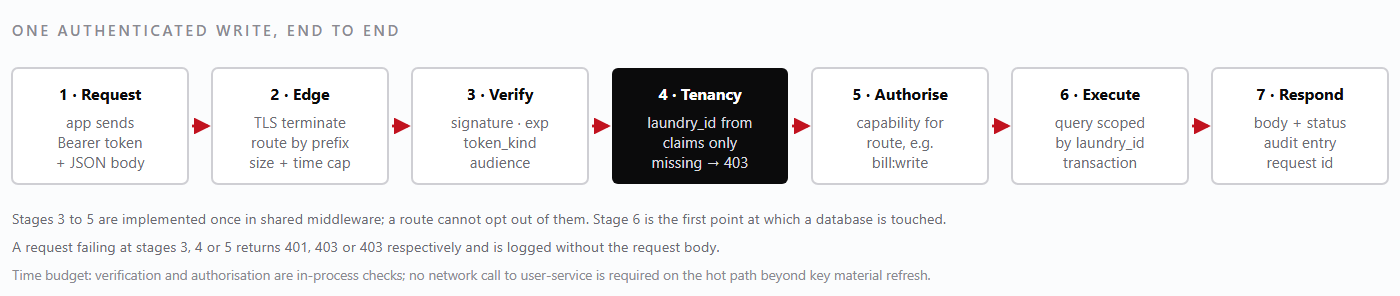
\includegraphics[width=\linewidth]{images/fig-02.png}
\caption{— Request lifecycle for an authenticated write. Tenancy resolution precedes authorisation, and no query is built before both have succeeded.Figure 2}
\end{figure}
\begin{center}\small
\begin{tabularx}{\linewidth}{|X|X|X|}
\hline
\rowcolor{lightgrey}
\textbf{Stage} & \textbf{Enforced by} & \textbf{On failure} \\ \hline
1 Request & Client HTTP wrapper & No token → the app redirects to sign-in without calling the API. \\ \hline
2 Edge & Reverse proxy & Oversized body → 413; TLS failure → connection refused; timeout → 504. \\ \hline
3 Verify & Auth middleware & Bad signature, expired token or wrong  → 401 with a generic message.\texttt{token\_kind} \\ \hline
4 Tenancy & Tenant dependency & No  in claims → 403. There is no unscoped fallback and no default tenant.\texttt{laundry\_id} \\ \hline
5 Authorise & Capability dependency & Capability not held for this laundry → 403, logged with the capability name. \\ \hline
6 Execute & Repository layer & Cross-tenant reference, stale version or duplicate key → 409 or 422; nothing is written. \\ \hline
7 Respond & Serialiser and logger & Serialisation error → 500 with a request id; the audit entry records the failure. \\ \hline
\end{tabularx}
\end{center}
The practical consequence is that a handler never has to ask “which laundry is this?”. It receives a resolved tenant context, or it is never called. That single decision removes an entire class of defect — the query that forgets its filter — because there is no filter to forget: the repository takes the tenant as a mandatory argument.

\section{2.5 The three-database model}
The platform separates its data into three MongoDB databases along ownership lines. The split is not cosmetic: it constrains what each service can see, it lets each store be backed up and restored on its own schedule, and it keeps a reporting query from ever competing with a counter sale for the same lock or connection pool.

Identity and tenancy — user\_dbHolds , , and . It is small, changes rarely, and is read on every sign-in. Its integrity is a precondition for everything else: if identity is wrong, every downstream decision is wrong. It is written only by user-service.userslaundriesmembershipsclient\_accounts

Operations — the bill\_service databaseHolds , , , , , , day-close records, dispatch records and the materialised monthly matrix. This is the largest and busiest store, written by every front end and read by dashboards, and it is the one whose loss stops the business trading.gate\_passesdeliveriesbillsshop\_billslinensreturns

2 · System Overview and ArchitectureLoveLaundry — System Manual

Accounting — laundry-managementHolds , , , , , and salary records. It follows accounting conventions: records are posted, not edited; periods are closed; and the ledger is the source of financial truth even when an operational figure disagrees.customerstransactionspaymentsexpensesemployeesitems

\subsection*{Rules that hold the model together}
\begin{itemize}
\item A service writes only its own collections. There is no shared collection and no “just this once” cross-write, because the second writer is always the one that skips a validation.\textbf{One writer per collection.}
\item Where a document needs data from another domain, it stores the identifier and the small denormalised fragment it needs at write time — a client name, a rate, a worker name — and treats that fragment as a snapshot, not a live reference.\textbf{No cross-database joins.}
\item Creating a delivery that references a gate pass checks that the pass exists ; a valid identifier from another laundry is rejected exactly like a fabricated one.\textbf{References are validated at the boundary.}\emph{in the same tenant}
\item user\_db first, operations second, accounting third — because operations records reference identity and accounting records reference operations. Chapter 10 uses this order in every restore procedure.\textbf{Restore order is fixed.}
\item Each store has its own RPO and retention, reflecting how much history each one must be able to reconstruct.\textbf{Backups are per database.}
\end{itemize}
\subsection*{Why not one database?}
A single database would be simpler to operate and harder to reason about. Three concerns drive the separation. First, blast radius: a runaway reporting aggregation in the operations store must not degrade sign-in. Second, retention: accounting records must survive longer and be restorable to a specific date without replaying operational churn. Third, authority: when an operational balance and an accounting balance disagree, the platform needs an unambiguous rule about which one is corrected — and that rule is only credible if the two live in different stores.

\begin{notebox}NoteThe three databases may run on the same MongoDB replica set in a small deployment. Separation is logical first and physical second; the ownership rules apply either way, and a future move to separate clusters requires no application change.\end{notebox}
\begin{center}\small
\begin{tabularx}{\linewidth}{|X|X|X|X|X|}
\hline
\rowcolor{lightgrey}
\textbf{Store} & \textbf{Write rate} & \textbf{Growth driver} & \textbf{Restore priority} & \textbf{Loss impact} \\ \hline
user\_db & Low & Users and memberships & 1 — first & Nobody can sign in; total outage \\ \hline
Operations & High & Daily passes, deliveries, scans & 2 — second & Trading stops; unbilled work \\ \hline
Accounting & Medium & Transactions and payroll & 3 — third & Reporting and settlement impaired \\ \hline
\end{tabularx}
\end{center}
2 · System Overview and ArchitectureLoveLaundry — System Manual

\section{2.6 Data ownership}
Ownership is the answer to two questions: which service may write this data, and which service must be consulted when it changes? The table below is the reference used during design reviews and incident triage.

\begin{center}\small
\begin{tabularx}{\linewidth}{|X|X|X|X|}
\hline
\rowcolor{lightgrey}
\textbf{Collection} & \textbf{Owner} & \textbf{Tenant key} & \textbf{Key fields and notes} \\ \hline
users & user-service & — & Identity: email, password hash, display name, status. Global to the platform, not tenant-scoped; authorisation comes from memberships. \\ \hline
laundries & user-service & \_id & The tenant record: name, status, plan, contact details. Its  is the  used everywhere else.\texttt{\_id}\texttt{laundry\_id} \\ \hline
memberships & user-service & laundry\_id & User ↔ laundry link with role and capability set. Copied as a snapshot into the token at sign-in. \\ \hline
client\_accounts & user-service & laundry\_id & Hotel logins: email, password hash, , status. Carries no staff role and no membership.\texttt{client\_name} \\ \hline
gate\_passes & bill\_service & laundry\_id & Client name, pass number, dates, item lines and quantities, status, linen tag references. \\ \hline
deliveries & bill\_service & laundry\_id & References gate pass lines; delivered quantities, delivery date, receiver, status. \\ \hline
bills & bill\_service & laundry\_id & Client name, period, line items, totals, balance, status. Immutable once issued; corrected by adjustment records. \\ \hline
shop\_bills & bill\_service & laundry\_id & Counter sales: number, lines, tender type, cashier, day-close reference. \\ \hline
linens & bill\_service & laundry\_id & Tag identifier, item type, current status, lifecycle events, last scan time and user. \\ \hline
returns & bill\_service & laundry\_id & Returned quantities and reasons, referencing the original delivery where one exists. \\ \hline
quotations & quotation-service & laundry\_id & Client name, line items, rates, validity, status. Converts to work, never directly to a bill. \\ \hline
workers & worker-service & laundry\_id & Worker identity, assignment, attendance. Names are denormalised onto operational records at write time. \\ \hline
customers, transactions, payments & laundry-management & laundry\_id & Accounting ledger. Payments posted here mirror operational payments; neither copy is edited in place. \\ \hline
expenses, salary, employees, items & laundry-management & laundry\_id & Cost side of the business and the priced item catalogue used when raising bills. \\ \hline
\end{tabularx}
\end{center}
\subsection*{Denormalisation, and why it is deliberate}
Operational documents copy small fragments of other domains at write time: a gate pass stores the  string, a delivery line stores the item description and rate, a bill stores the client's billing name. This is not a violation of ownership: it is how the platform avoids cross-database joins and keeps historical documents readable after the source record changes.\texttt{client\_name}

The rule is that a copied fragment is a . Renaming a client does not rewrite last month's invoices; it changes what future documents carry. The same applies to rates: a bill raised at an old rate remains correct at that rate, and a re-price is a new document, not an edit.\emph{snapshot of what was true when the document was written}

2 · System Overview and ArchitectureLoveLaundry — System Manual

\subsection*{What each service may read}
\begin{itemize}
\item A service reads its own collections freely, always with the tenant filter applied.
\item A service reads another domain's data only through that domain's HTTP interface, with the caller's own token.
\item Reporting reads are the exception that proves the rule: dashboards and the monthly matrix are computed inside bill\_service from its own collections, not by reaching into accounting.
\end{itemize}
\begin{notebox}WarningA direct database read across domains — for example, joining  to  inside a single aggregation — couples two services' schemas and breaks the restore-order guarantees in Chapter 10. Use the owning service's API.\texttt{bills}\texttt{payments}\end{notebox}
\section{2.7 JWT and tenancy flow}
Tenancy is established once, at sign-in, and carried in the token thereafter. The sequence below shows a staff sign-in and the first authenticated read that follows it.

\begin{figure}[htbp]
\centering
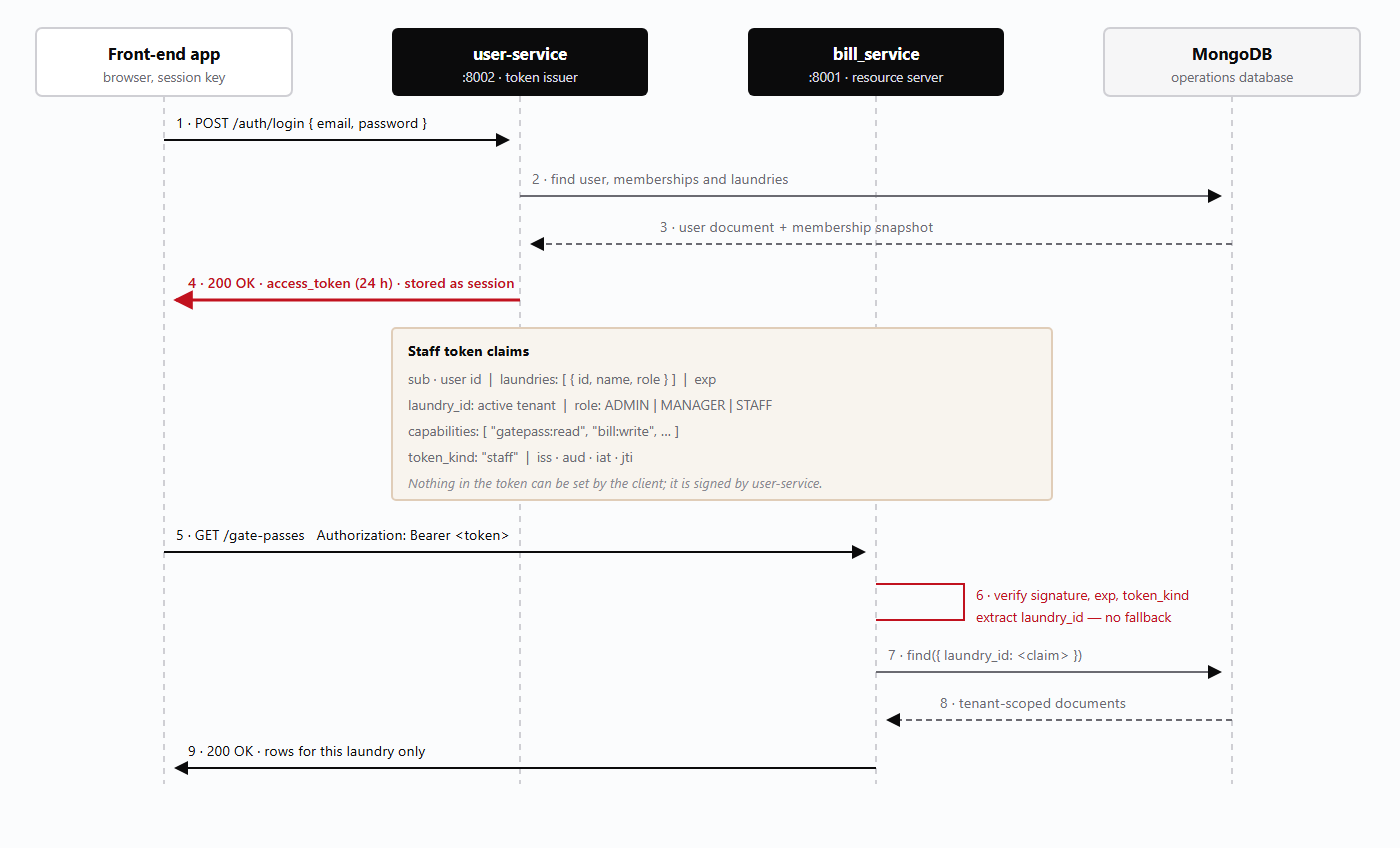
\includegraphics[width=\linewidth]{images/fig-03.png}
\caption{— JWT issuance and tenancy resolution. The token is issued once, verified on every request, and is the sole carrier of .Figure 3laundry\_id}
\end{figure}
\subsection*{What the token is, and is not}
2 · System Overview and ArchitectureLoveLaundry — System Manual

The token is a signed statement of identity, tenant and capability. It is not a session record: the services keep no session table, which is why a stolen token remains usable until it expires and why expiry is kept short — 24 hours for staff, 12 hours for hotel clients. Revocation is therefore a matter of disabling the user or the client account and rotating the signing key, not of deleting a row; Chapter 3.6 describes the procedure.

The  claim is a snapshot of the user's memberships at sign-in. It exists so that downstream services can resolve a laundry name without calling user-service, and so that a session can switch tenants only by signing in again — which is the intended behaviour, because a silent tenant switch is exactly the mistake the design is trying to prevent.\texttt{laundries}

\begin{notebox}NoteA user with memberships in two laundries has two valid tenants, but a token names exactly one. Switching laundry re-authenticates. This is a deliberate trade of convenience for certainty.\end{notebox}
\section{2.8 Hotel client-account isolation}
Hotels are the platform's most sensitive external readers, and the design that protects them is deliberately unusual.  There is no  collection and no hotel tenant. A hotel is the  string carried on gate passes, deliveries, bills and quotations — a value that already existed in the operational data before the hotel portal was built.\textbf{A hotel is not an entity.}\texttt{hotels}\texttt{client\_name}

Hotel logins live in a separate  collection in user-service. A client account records an email, a password hash, a status, the laundry it belongs to and the  it may see. It holds no role, no membership and no capability list, because a hotel user is not staff and must never be granted a staff permission by accident.\texttt{client\_accounts}\texttt{client\_name}

\subsection*{How the isolation actually works}
When a hotel signs in through , user-service issues a token with a deliberately different shape. It carries  and . Instead it carries:\texttt{POST /client/auth/login}\textbf{no \texttt{laundry\_id}}\textbf{no  claim\texttt{laundries}}

\begin{verbatim}
{
  "sub": "<client account id>",
  "token_kind": "client",
  "client_scope": { "laundry_id": "<tenant>", "client_name": "<hotel name>" },
  "exp": <issued + 12 hours>
}
\end{verbatim}
Staff endpoints resolve the tenant from  or from the  membership snapshot. A client token has neither, so those endpoints reject it automatically — not because someone remembered to add a check, but because the tenant dependency cannot resolve a context and therefore fails closed. There is no path by which a hotel token can reach a staff handler and be treated as a member of staff.\texttt{laundry\_id}\texttt{laundries}

Hotel portal endpoints live under  and read  explicitly. Every query filters on   and . Filtering on the name alone would be unsafe — two laundries could serve hotels with the same name — and filtering on the laundry alone would expose every hotel's data to every other hotel. Requiring both makes the pair the effective scope.\texttt{/client-portal}\texttt{client\_scope}\textbf{both}\texttt{laundry\_id}\texttt{client\_name}

2 · System Overview and ArchitectureLoveLaundry — System Manual

\begin{center}\small
\begin{tabularx}{\linewidth}{|X|X|X|}
\hline
\rowcolor{lightgrey}
\textbf{Claim} & \textbf{Staff token} & \textbf{Hotel client token} \\ \hline
token\_kind & "staff" & "client" \\ \hline
laundry\_id & Present — the active tenant & \textbf{Absent by design} \\ \hline
laundries & Membership snapshot with roles & \textbf{Absent by design} \\ \hline
client\_scope & Absent & \{ laundry\_id, client\_name \} \\ \hline
role / capabilities & Role plus resolved capability list & None — portal endpoints check scope only \\ \hline
Lifetime & 24 hours & 12 hours \\ \hline
Accepted by & Staff routes on all services & routes only\texttt{/client-portal} \\ \hline
Rejected by & routes\texttt{/client-portal} & Every staff route, automatically \\ \hline
\end{tabularx}
\end{center}
\subsection*{Why not give hotels a tenant?}
Making a hotel a tenant would multiply the identity surface: every hotel would need a laundry, a membership, a role and a capability set, and every operational query would need a second scoping rule to decide whether the caller was staff or client. It would also make the existing data wrong, because the operational documents already carry  and no hotel identifier.\texttt{client\_name}

The chosen design keeps one tenant per laundry and one extra dimension —  — that is already present in the data. The cost is that hotel accounts are managed separately from staff accounts, which Chapter 8.3 covers. The benefit is that the two classes of token cannot be confused, and that a defect in hotel-facing code cannot escalate into staff authority.\texttt{client\_name}

\begin{notebox}WarningAdding  to a client token to “simplify” a query destroys this isolation: the token would then satisfy the staff tenant dependency. Hotel portal code must read , never a top-level tenant claim.\texttt{laundry\_id}\texttt{client\_scope}\end{notebox}
\section{2.9 Deployment topology}
The reference deployment is a single application host behind a TLS-terminating reverse proxy, with MongoDB on a separate host and backups written to object storage. This is the topology the recovery procedures in Chapter 10 assume.

2 · System Overview and ArchitectureLoveLaundry — System Manual

\begin{figure}[htbp]
\centering
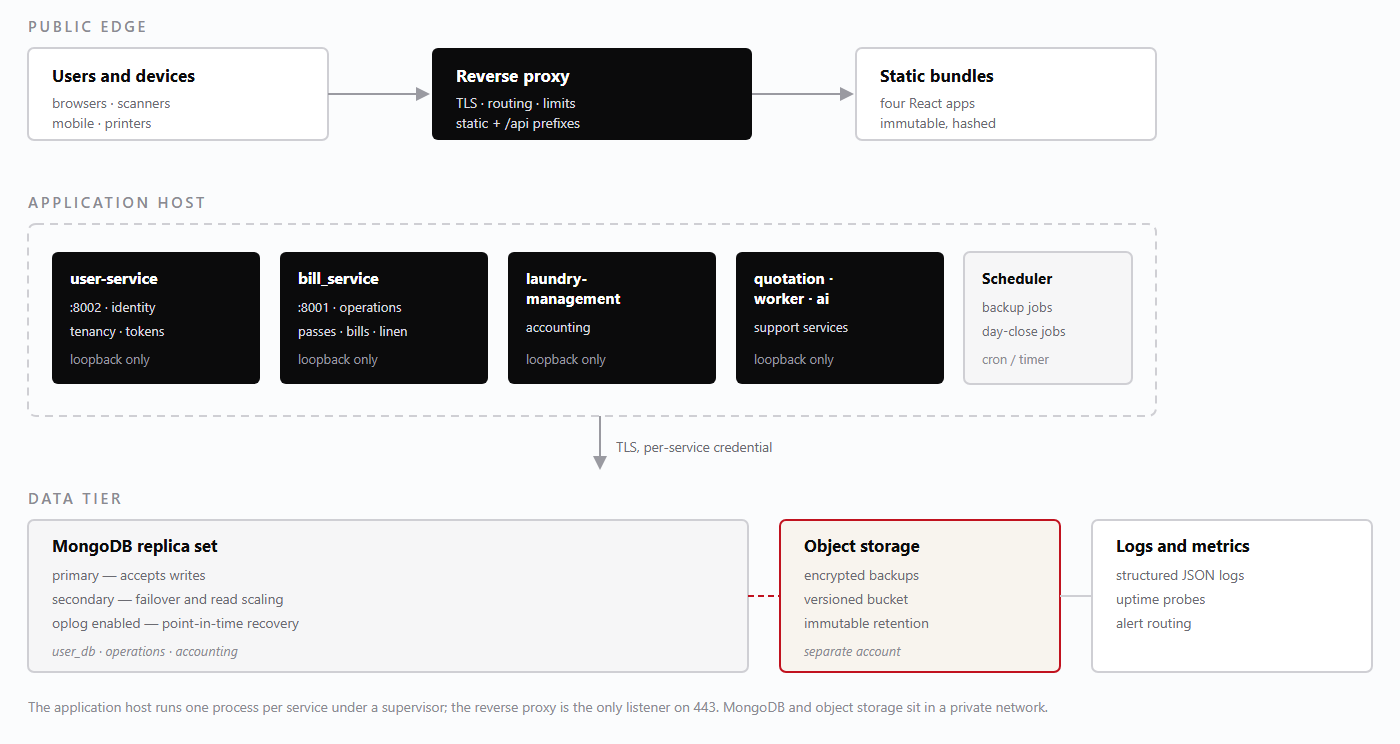
\includegraphics[width=\linewidth]{images/fig-04.png}
\caption{— Reference deployment topology: proxy at the edge, services on loopback, replica set and object storage behind a private network.Figure 4}
\end{figure}
\subsection*{Operating assumptions}
\begin{itemize}
\item The reference deployment accepts a single host as a single point of failure for compute, mitigated by documented rebuild steps and by the fact that all state lives in MongoDB and object storage.\textbf{Single application host.}
\item Three members are recommended: one primary, one secondary for failover, and one arbiter or a third data-bearing member. The oplog is what makes point-in-time recovery possible.\textbf{MongoDB replica set.}
\item Backup files are written to an object-storage bucket in a separate account with immutability enabled, so that a compromised application host cannot delete its own history.\textbf{Backups off-host.}
\item Front-end bundles can be rebuilt from source at any time; they are not backed up as data, only as release artefacts.\textbf{Static assets are disposable.}
\end{itemize}
\section{2.10 Technology stack}
The stack is deliberately conventional. Every component is widely used, well documented and replaceable, because a laundry platform is maintained by a small team and must remain legible to whoever inherits it.

2 · System Overview and ArchitectureLoveLaundry — System Manual

\begin{center}\small
\begin{tabularx}{\linewidth}{|X|X|X|}
\hline
\rowcolor{lightgrey}
\textbf{Layer} & \textbf{Technology} & \textbf{Why it was chosen} \\ \hline
Front-end framework & React 19 & Component model that suits form-heavy operational screens; the largest available hiring and support pool. \\ \hline
Language (front end) & TypeScript & Types on API payloads catch the field-name mistakes that otherwise reach production as blank columns. \\ \hline
Build tool & Vite 8 & Fast development server, simple static output, environment injection at build time. \\ \hline
Styling & Tailwind CSS 4 & Consistent spacing and colour without a bespoke component library; small CSS payload. \\ \hline
Service framework & FastAPI (Python) & Typed request models, automatic OpenAPI schema, dependency injection that suits auth and tenancy middleware. \\ \hline
Database & MongoDB & Document model matches the shape of gate passes and bills, whose line items vary by client; flexible schema for a business that evolves. \\ \hline
Auth & JWT (signed bearer tokens) & Stateless verification at every service; claims carry tenancy so no lookup is needed on the hot path. \\ \hline
Mobile & Flutter (LoveMobi) & One codebase for Android and iOS for owners and managers. \\ \hline
Hosting & Linux host, reverse proxy, object storage & Simple, reproducible, and recoverable without provider-specific tooling. \\ \hline
\end{tabularx}
\end{center}
\subsection*{Version policy}
Front-end dependencies are pinned in the lockfile and upgraded deliberately, one minor version at a time, with a build and a smoke test after each step. Major upgrades — such as the move to React 19 and Tailwind 4 — are treated as projects: they are scheduled, tested against the four applications and released together, because a split across applications would leave staff switching between two visual languages.

Python service dependencies are pinned in the requirements file per service. A service may be upgraded independently, which is one of the practical benefits of the split: bill\_service can stay on a proven dependency set while a lower-risk service takes a newer one.

\subsection*{What the stack deliberately excludes}
\begin{itemize}
\item The applications cache responses for resilience (Chapter 11.4) but never treat the cache as a source of truth.\textbf{No client-side database.}
\item Cross-service side effects use durable outbox records and retries rather than introducing an operational dependency the team would have to run.\textbf{No message broker in the reference deployment.}
\item The applications are internal tools behind authentication; search-engine visibility is irrelevant and a static bundle is simpler to secure.\textbf{No server-side rendering.}
\item Four separate deployments achieve independence without a runtime composition layer.\textbf{No micro-front-end framework.}
\end{itemize}
2 · System Overview and ArchitectureLoveLaundry — System Manual

\begin{center}\small
\begin{tabularx}{\linewidth}{|X|X|X|}
\hline
\rowcolor{lightgrey}
\textbf{Component} & \textbf{Version line} & \textbf{Notes} \\ \hline
Node.js (build) & Current LTS & Build-time only; the runtime artefact is static files. \\ \hline
Python & 3.11+ & Service runtime; virtual environment per service. \\ \hline
MongoDB & 6.0+ & Replica set required for transactions and oplog-based recovery. \\ \hline
React / Vite / Tailwind & 19 / 8 / 4 & Aligned across all four applications. \\ \hline
\end{tabularx}
\end{center}
\begin{notebox}NoteExact pinned versions are recorded in the lockfiles and in each service's requirements file. This manual states version lines, not patch numbers, because patch numbers change with every security update and a manual that quotes them is wrong within weeks.\end{notebox}
\textsc{\small\color{crimson}2.11 · Service dependencies}\par\medskip
\section*{Service dependency graph}
Which service calls which, and what fails when an arrow breaks.

\begin{figure}[htbp]
\centering
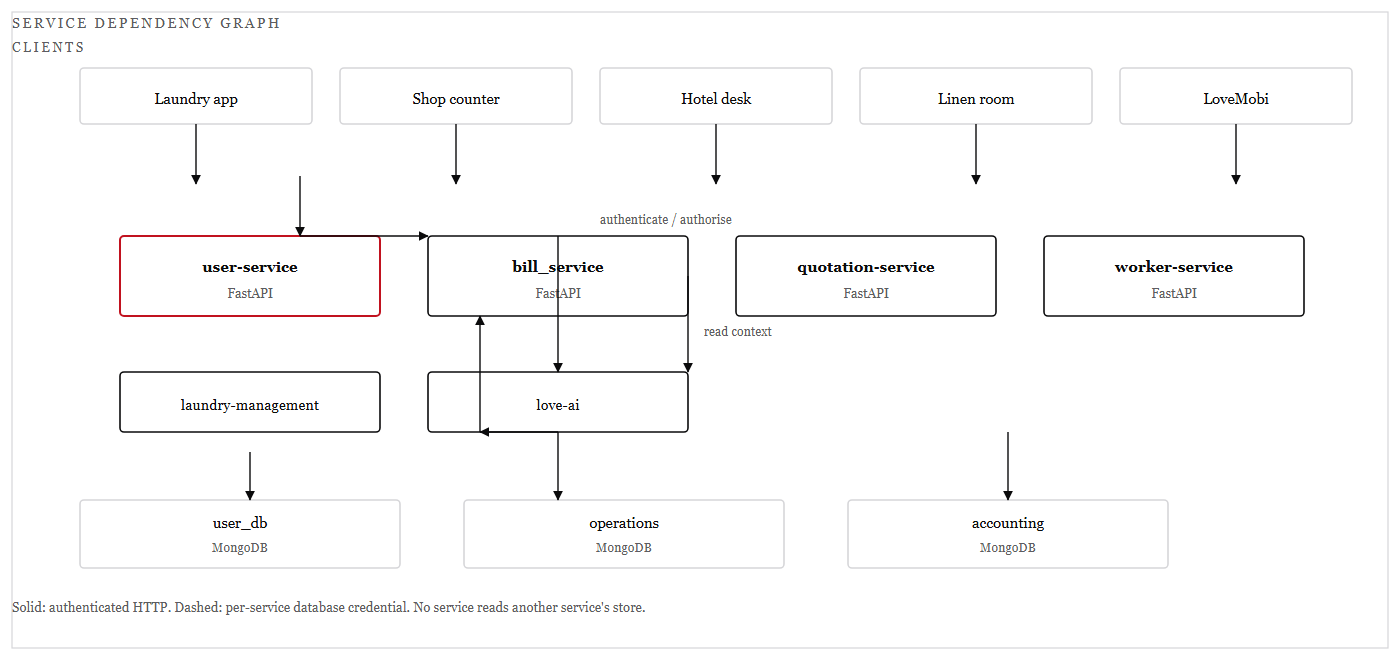
\includegraphics[width=\linewidth]{images/fig-05.png}
\caption{— Service dependency graph, drawn as a line diagram: authenticated HTTP between services, per-service credentials to each store.Figure 5}
\end{figure}
The graph is deliberately shallow. Clients talk to services; services talk to user-service for identity and to each other only where a business operation genuinely spans two domains. There is no service that every other service depends on except the identity authority, and that is the single point the platform accepts.

Reading the graph during an incident is a matter of following the arrows backwards from the symptom. A shop counter that cannot take payment is not a shop problem: the arrow from shop-app to bill\_service is broken, and the first question is whether bill\_service is reachable or merely slow.

2 · System Overview and ArchitectureLoveLaundry — System Manual

\textsc{\small\color{crimson}2.12 · Tenancy decision flow}\par\medskip
\section*{Tenancy decision flow}
Five checks, in order, before a single document is read.

\begin{figure}[htbp]
\centering
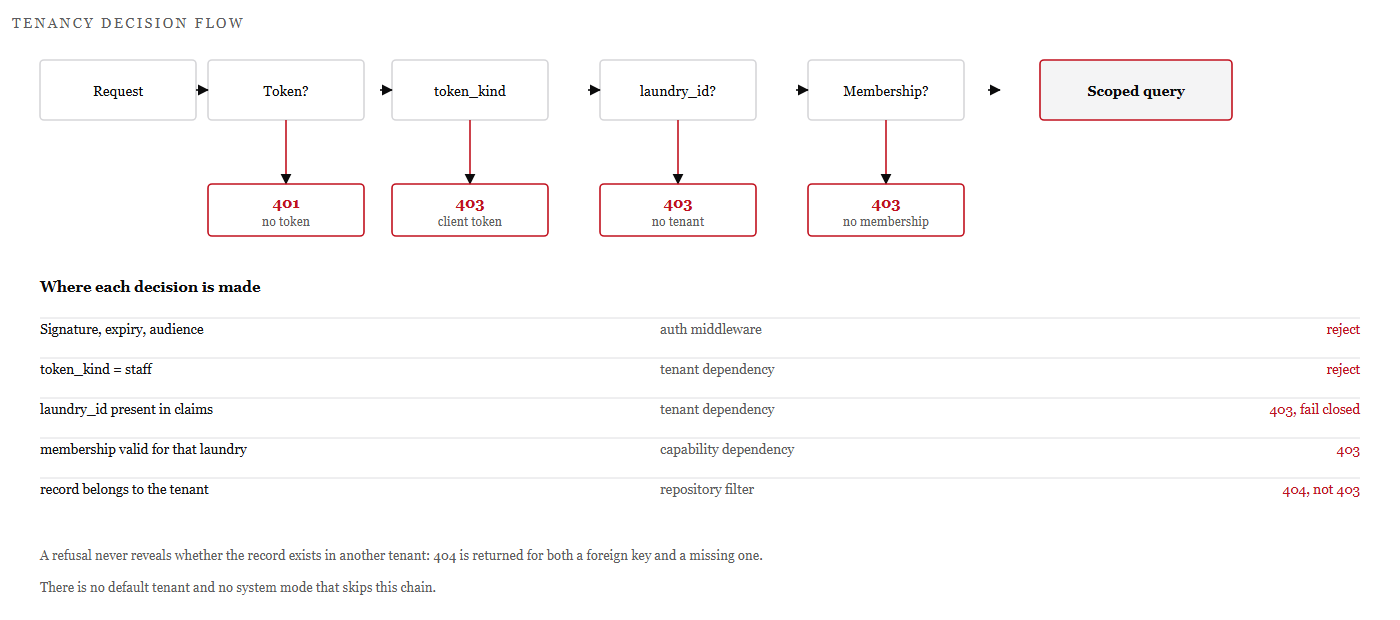
\includegraphics[width=\linewidth]{images/fig-06.png}
\caption{— The tenancy decision chain. Each failure returns before the next check runs.Figure 6}
\end{figure}
Chapter 3 sets out the enforcement rules in full from page 34. Tenancy is not a filter applied at the end of a query; it is a sequence of decisions that must all succeed before a query is built. The order matters: identity before token kind, token kind before tenant, tenant before membership, membership before the record itself.

The practical consequence is that a handler never asks which laundry is calling. It receives a resolved tenant context or it is never invoked, which removes the class of defect in which a developer forgets a filter.

\begin{notebox}RuleA refusal never distinguishes a foreign record from a missing one. Both return not-found, so the endpoint cannot be used to enumerate another tenant's documents.\end{notebox}
\textsc{\small\color{crimson}2.13 · Failure domains}\par\medskip
\section*{Deployment topology and failure domains}
What fails together, and why the backup must live outside the blast radius.

2 · System Overview and ArchitectureLoveLaundry — System Manual

\begin{figure}[htbp]
\centering
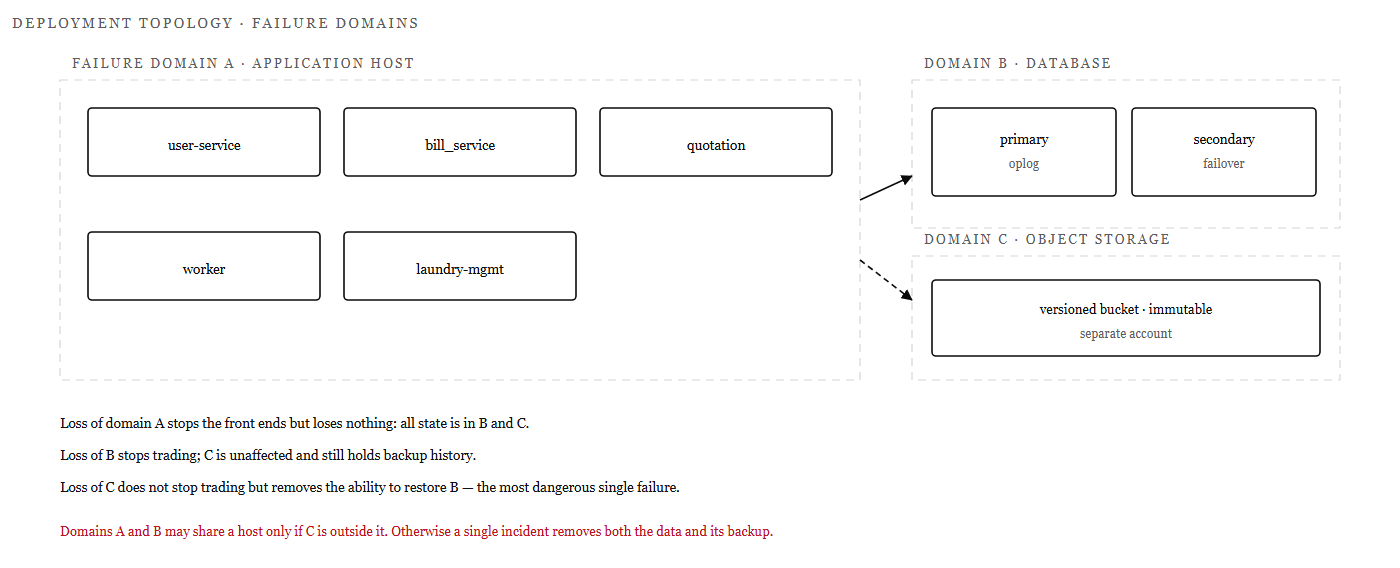
\includegraphics[width=\linewidth]{images/fig-07.png}
\caption{— Failure domains in the reference deployment: application host, database replica set, object storage.Figure 7}
\end{figure}
The topology is drawn as three domains rather than three tiers, because the question that matters in a disaster is not what talks to what but what disappears together. The application host is disposable: it holds no state and can be rebuilt from the deployment steps.

The database is the domain that stops trade, and object storage is the domain that makes recovery possible. Keeping them in separate accounts is the control that prevents one compromised credential from removing both the data and its history.

\begin{notebox}RuleIf the database and its backups share an account, ransomware has one target, not two. Separation of accounts is a recovery control, not an administrative preference.\end{notebox}
\textsc{\small\color{crimson}Part One · Security Model}\par\medskip
\chapter{Security Model}
\begin{quote}\itshape Who can sign in, what they may do, and why one laundry can never read another's records.\end{quote}
\section{3.1 Authentication}
The platform recognises three kinds of principal, and each has its own sign-in path. Staff — owners, managers, supervisors and counter staff — sign in against user-service with an email and password and receive a 24-hour staff token. Linen-room staff use the same path with linen-room roles attached to their membership. Hotel clients sign in against a separate endpoint with a separate collection and receive a 12-hour client token with a different claim shape. There is no anonymous access to any business endpoint.

\begin{center}\small
\begin{tabularx}{\linewidth}{|X|X|X|X|}
\hline
\rowcolor{lightgrey}
\textbf{Principal} & \textbf{Endpoint} & \textbf{Lifetime} & \textbf{Token characteristics} \\ \hline
Staff (laundry app, shop) & POST /auth/login & 24 hours & , ,  snapshot, role and capabilities\texttt{token\_kind: "staff"}\texttt{laundry\_id}\texttt{laundries} \\ \hline
Linen-room staff & POST /auth/login & 24 hours & Same as staff, with  or  role and linen capabilities\texttt{LINEN\_SUPERVISOR}\texttt{HOUSEKEEPER} \\ \hline
Hotel client & POST /client/auth/login & 12 hours & , , no tenant claim, no capabilities\texttt{token\_kind: "client"}\texttt{client\_scope} \\ \hline
\end{tabularx}
\end{center}
\subsection*{Credential handling}
3 · Security ModelLoveLaundry — System Manual

\begin{itemize}
\item Only a salted, slow hash is persisted. The plaintext exists for the duration of the request and is never logged, echoed or written to an audit record.\textbf{Passwords are never stored.}
\item A wrong password and an unknown email produce the same message and the same shape of failure, so that the endpoint cannot be used to enumerate accounts.\textbf{Sign-in responses are deliberately uniform.}
\item A disabled user or client account cannot obtain a token; a token already issued for an account that is later disabled is rejected once the account status cache is refreshed, and immediately on the next sign-in attempt.\textbf{Status is checked at sign-in and at use.}
\item If a user holds memberships in more than one laundry, the session is bound to one. Switching requires re-authentication — there is no endpoint that changes  inside a live token.\textbf{Tenant is chosen at sign-in.}\texttt{laundry\_id}
\item There is no code path that converts a  record into a membership, and no endpoint that issues a staff token for a client account.\textbf{Client accounts cannot be promoted.}\texttt{client\_accounts}
\end{itemize}
\subsection*{Session handling in the front ends}
Each application keeps its token under its own key:  for the shop,  for the hotel desk and  for the linen room. Separate keys mean that a supervisor who opens the shop app and the linen app in the same browser holds two independent sessions and cannot accidentally act in the wrong one. On a 401 the application clears its own key and returns to sign-in; it does not retry with the same token and it does not fall back to another stored session.\texttt{ll\_shop\_session}\texttt{ll\_hotel\_session}\texttt{ll\_linen\_session}

\begin{notebox}WarningToken lifetime is a security control, not a convenience setting. Extending the staff lifetime to “avoid signing in every morning” lengthens the window in which a stolen token is usable, because there is no server-side session to revoke. Disable the account or rotate the signing key instead.\end{notebox}
\subsection*{What authentication does not do}
Authentication establishes who is calling. It does not establish what they may do — that is authorisation, covered next — and it does not by itself confine them to a tenant, which is why the tenant dependency runs as a separate stage and fails closed. A valid token with no resolvable tenant is useless: it authenticates a caller the platform then refuses to serve.

\section{3.2 Roles and capabilities}
Authorisation is capability-based. A role is a named bundle of capabilities, and every protected endpoint declares the capability it requires. Adding a role means adding a bundle; it never means adding an  branch inside a handler. The complete matrix is in Appendix B; this section explains the roles and the reasoning behind the bundles.\texttt{if role == …}

3 · Security ModelLoveLaundry — System Manual

\begin{center}\small
\begin{tabularx}{\linewidth}{|X|X|X|}
\hline
\rowcolor{lightgrey}
\textbf{Role} & \textbf{Applies to} & \textbf{Intent} \\ \hline
PLATFORM\_ADMIN & Platform & Superset of ADMIN. Creates laundries, provisions the first administrator of each tenant, and can act across tenants for support purposes. Held by the platform operator, not by laundry staff. \\ \hline
ADMIN & One laundry & Full control of a single tenant: users and memberships, hotel client accounts, configuration, day close, all operational and financial modules. \\ \hline
MANAGER & One laundry & Runs the operation: gate passes, deliveries, bills, payments, quotations, reports and day close. May not create users or change tenant configuration. \\ \hline
STAFF & One laundry & Day-to-day operational entry: gate passes, deliveries, bills and read-only dashboards. No payment posting, no reports, no administration. \\ \hline
HOTEL\_ADMIN & One client account & Hotel-side administrator: sees the property's full portal, including invoices and statements. Cannot see any other client of the laundry. \\ \hline
HOTEL\_MANAGER & One client account & Hotel-side operational reader: gate passes, deliveries and invoices for the property. Statements are available; account settings are not. \\ \hline
LINEN\_SUPERVISOR & One laundry & Owns the linen room: scanning, status transitions, inventory, discrepancies, tag printing and the retirement of items. \\ \hline
HOUSEKEEPER & One laundry & Scans collection and receipt, and moves items through wash and press. Cannot retire, mark missing or print tags. \\ \hline
\end{tabularx}
\end{center}
\subsection*{Capabilities}
Capabilities are strings of the form . They are carried in the token, checked by a dependency on each route, and used by the front ends to decide which controls to render. The set in use is:\texttt{resource:action}

\begin{center}\small
\begin{tabularx}{\linewidth}{|X|X|X|}
\hline
\rowcolor{lightgrey}
\textbf{Capability} & \textbf{Grants} & \textbf{Notes} \\ \hline
gatepass:read & List and view gate passes & Scoped to the session tenant and, for hotel tokens, to \texttt{client\_name} \\ \hline
gatepass:write & Create, edit, cancel gate passes & Cancel is a status change, never a delete \\ \hline
delivery:read & List and view deliveries & Includes partial deliveries \\ \hline
delivery:write & Record and amend deliveries & Amendments require a reason and are audited \\ \hline
bill:read & View bills and balances & Hotel portal uses scope, not this capability \\ \hline
bill:write & Raise bills and adjustments & Issued bills are immutable \\ \hline
payment:read & View payments and receipts &  \\ \hline
payment:write & Post payments and reversals & Never granted to STAFF \\ \hline
linen:read & View tags, inventory and discrepancies &  \\ \hline
linen:write & Change tag status, retire items & Retirement is supervisor-only \\ \hline
linen:scan & Submit scan events & Separate from write so scanners can be restricted \\ \hline
dashboard:read & View operational dashboards & Totals respect tenant scope only \\ \hline
report:read & View reports and the monthly matrix & Manager and above \\ \hline
\end{tabularx}
\end{center}
3 · Security ModelLoveLaundry — System Manual

\subsection*{Why capabilities rather than roles in code}
Role names are a poor thing to check inside a handler, because the business will always want one more variation — a senior housekeeper who may retire items, a counter supervisor who may post payments. With capabilities, that variation is a bundle change in one place, and the audit answer is a capability the user held rather than a job title interpreted somewhere in code.

\section{3.3 Tenant isolation rules}
Tenant isolation is the single most important property of the platform, and it is enforced by construction rather than by discipline. The rules below are stated as invariants: each one is either true of every request or the request fails.

\begin{center}\small
\begin{tabularx}{\linewidth}{|X|X|X|}
\hline
\rowcolor{lightgrey}
\textbf{\#} & \textbf{Invariant} & \textbf{How it is enforced} \\ \hline
1 & The tenant is read only from verified JWT claims. & Tenant dependency reads  from the decoded token. No request field is consulted for tenancy.\texttt{laundry\_id} \\ \hline
2 & Every query carries the tenant filter. & Repositories take the tenant as a required argument; there is no repository method that omits it. \\ \hline
3 & A missing tenant fails closed. & No claim → 403 before any handler runs. There is no default tenant and no unscoped fallback. \\ \hline
4 & Cross-tenant references are rejected. & Creating a delivery against a gate pass from another laundry returns 404 or 422 — the referenced document is treated as non-existent. \\ \hline
5 & Identifier lookups are tenant-scoped. & A valid identifier from another tenant behaves exactly like a fabricated one; the query never runs without the filter. \\ \hline
6 & Aggregations and reports are scoped. & Dashboard and matrix pipelines begin with a  on , never with a global scan.\texttt{\$match}\texttt{laundry\_id} \\ \hline
7 & Hotel reads require both keys. & queries filter on    from .\texttt{/client-portal}\texttt{laundry\_id}\emph{and}\texttt{client\_name}\texttt{client\_scope} \\ \hline
8 & Staff routes reject client tokens. & Client tokens carry no  and no  claim, so the tenant dependency cannot resolve and the request fails.\texttt{laundry\_id}\texttt{laundries} \\ \hline
\end{tabularx}
\end{center}
\subsection*{How a violation surfaces}
The platform deliberately does not distinguish “this record belongs to someone else” from “this record does not exist”. Both produce the same 404 or 422. The reason is that a different response would confirm the existence of another tenant's data, which is itself a leak: an attacker could enumerate identifiers and learn how many gate passes a competitor processes.

At the query level the filter is not applied as a post-processing step. A request for  compiles to a lookup on . If the identifier exists in another tenant, the query returns nothing, the handler raises not-found, and no document is ever loaded into memory.\texttt{/gatepasses/\{id\}}\texttt{\{ \_id: id, laundry\_id: <claim> \}}

\subsection*{Where tenancy is checked, end to end}
3 · Security ModelLoveLaundry — System Manual

\begin{itemize}
\item user-service resolves memberships and refuses to issue a token for a laundry the user does not belong to.\textbf{At sign-in:}
\item the tenant dependency extracts and validates the claim, then exposes a tenant context object to the handler.\textbf{On every request:}
\item the tenant is part of the query signature, so a handler cannot call a data access method without supplying it.\textbf{In every repository call:}
\item new documents have  stamped from the context, never from the payload. A payload that includes  is rejected rather than trusted.\textbf{In every write:}\texttt{laundry\_id}\texttt{laundry\_id}
\item the caller's token is forwarded, so the callee applies the same claim and cannot be tricked into a wider scope.\textbf{In cross-domain calls:}
\end{itemize}
\subsection*{Testing the invariant}
Tenancy is covered by explicit tests in both service suites: a request without a tenant claim must fail, a request with a foreign identifier must return not-found, a payload carrying  must be rejected, and a client token must be refused by staff routes. These are regression tests, not exploratory ones — they exist because the invariant is the product's central promise, and a refactor that quietly weakens it would otherwise pass every functional test.\texttt{laundry\_id}

\begin{notebox}WarningNever add a “system” or “service” flag that skips the tenant dependency. If an internal job needs cross-tenant access, it must iterate tenants explicitly, one scoped operation at a time, so that each unit of work has a named tenant in its logs.\end{notebox}
\section{3.4 Encryption at rest}
Sensitive fields are encrypted before they reach MongoDB, using envelope encryption with AES-256-GCM. The database stores ciphertext, an initialisation vector and an authentication tag; it never stores the key that could decrypt them. The design has three parts: a per-document data key, a key-encryption key that wraps it, and a deterministic search token that allows equality lookups without decryption.

3 · Security ModelLoveLaundry — System Manual

\begin{figure}[htbp]
\centering
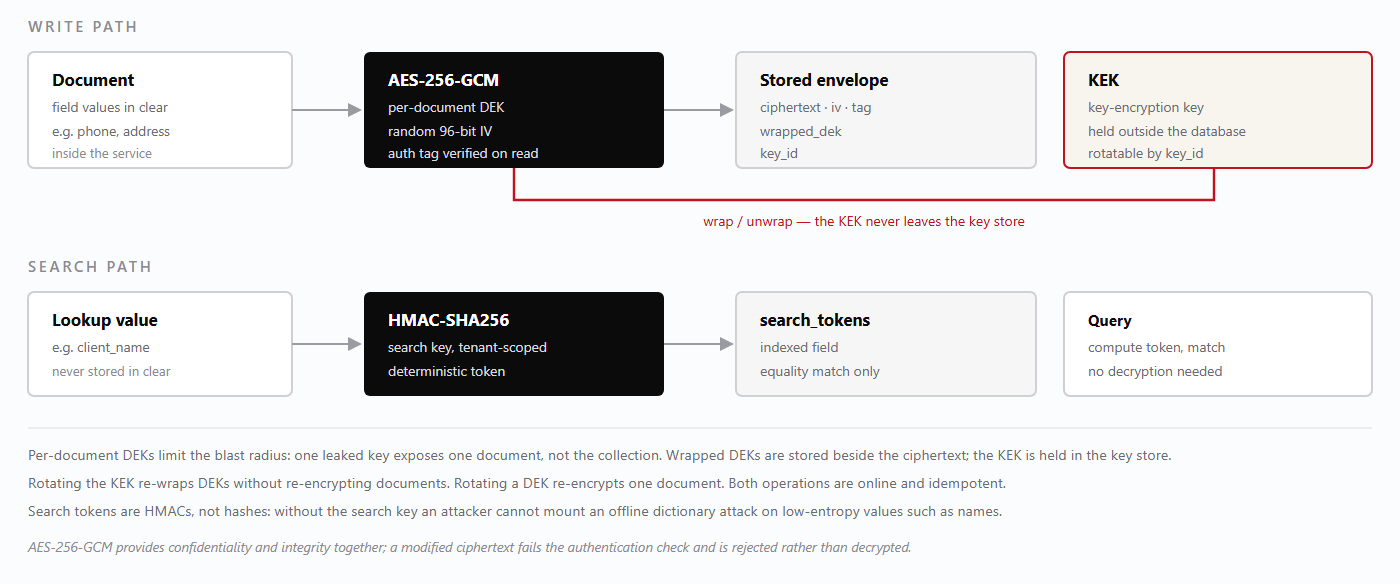
\includegraphics[width=\linewidth]{images/fig-08.png}
\caption{— Envelope encryption at rest, with a separate deterministic path for equality search.Figure 8}
\end{figure}
\subsection*{The three parts}
Each document that contains sensitive fields gets its own 256-bit data encryption key. The key is used once to encrypt the sensitive values with AES-256-GCM, a fresh 96-bit initialisation vector per encryption, and the resulting authentication tag is stored with the ciphertext. Reading the document requires the tag to verify; a tampered field fails rather than returning plausible garbage.\textbf{Per-document data key.}

The data keys are themselves encrypted — wrapped — by a key-encryption key that is held outside the database, in the environment's key store or secret manager. The database therefore contains wrapped keys that are useless without the KEK. A stolen database backup yields ciphertext and wrapped keys, not plaintext.\textbf{Key-encryption key.}

Encrypted values cannot be matched with a  or a range query, and the platform does not pretend otherwise. Where equality lookup is required — a client name, an account reference — the service also stores an HMAC-SHA256 token computed with a tenant-scoped search key. Queries match the token, never the ciphertext. Because the input space of names is small, a plain hash would be reversible by dictionary attack; an HMAC with a secret key is not.\textbf{Search tokens.}\texttt{\$regex}

\subsection*{What is encrypted, and what is not}
Encryption is applied to personal and commercial identifiers: client contact details, addresses, account references and free-text notes that may contain personal data. Operational keys — identifiers, dates, statuses, quantities and amounts — remain in clear because they are required for indexing, sorting, aggregation and reconciliation, and because encrypting them would make the monthly matrix impossible without decrypting every document in memory. The boundary is deliberate and documented so that a future reviewer does not assume more protection than exists.

\begin{notebox}Key custodyLosing the KEK loses the encrypted fields permanently; there is no recovery path by design. The KEK is therefore backed up separately from the database, under a different access policy, and its escrow is tested in the restore drill described in Chapter 10.7.\end{notebox}
3 · Security ModelLoveLaundry — System Manual

\section{3.5 Transport, audit and rate limiting}
\subsection*{Transport}
All traffic between clients and services, and between services and MongoDB, is encrypted in transit. The reverse proxy terminates TLS 1.2 or 1.3 with modern cipher suites, redirects plain HTTP to HTTPS, and sets HTTP Strict Transport Security so that a browser refuses to downgrade on subsequent visits. Certificates are issued for the platform's hostnames and renewed automatically; expiry is monitored as an alert.

Internal calls stay inside the private network and are authenticated with the caller's token. MongoDB connections use TLS with a per-service credential, so a service can read only the database it owns. The only public listener is the proxy on port 443.

\subsection*{Audit}
Security-relevant events are recorded with the actor, the tenant, the action, the target and the outcome. Audit records are append-only and are written even when the action fails, because a rejected attempt is often more interesting than a successful one.

\begin{center}\small
\begin{tabularx}{\linewidth}{|X|X|}
\hline
\rowcolor{lightgrey}
\textbf{Event class} & \textbf{Recorded detail} \\ \hline
Sign-in success and failure & Email, tenant where resolvable, source address, user agent, outcome. Failures never include the submitted password. \\ \hline
Token rejection & Reason class only — expired, bad signature, wrong token kind, unresolvable tenant — with the route and request id. \\ \hline
Authorisation denial & Required capability, the caller's role, the route, the tenant. \\ \hline
Privileged writes & User creation, role change, membership change, client account creation or status change, day close, bill issue, payment post and reversal. \\ \hline
Data correction & Amendment of a delivery, cancellation of a gate pass, adjustment of a bill — with reason and before/after summary. \\ \hline
Administrative access & Backup restore, key rotation, environment change, tenant creation. \\ \hline
\end{tabularx}
\end{center}
Audit entries are structured JSON written to the log pipeline with a retention period longer than the operational data they describe. They are not editable through any application route: no endpoint updates or deletes an audit record, and the application's storage credential is append-only.

\subsection*{Rate limiting}
Rate limits protect the sign-in endpoints from credential stuffing and the write endpoints from runaway clients — a scanner stuck in a retry loop, or a page that resubmits a bill. Limits are applied per source address and per account at the proxy and again in the service, so that a misconfigured proxy does not remove the protection.

3 · Security ModelLoveLaundry — System Manual

\begin{center}\small
\begin{tabularx}{\linewidth}{|X|X|X|}
\hline
\rowcolor{lightgrey}
\textbf{Class} & \textbf{Applies to} & \textbf{Behaviour on breach} \\ \hline
Authentication & , \texttt{/auth/login}\texttt{/client/auth/login} & 429 with a retry hint; repeated breaches escalate to a temporary block and an alert \\ \hline
Read & List and detail routes & 429; clients back off with jitter \\ \hline
Write & Creates, updates, payments & 429 before the handler; no partial write occurs \\ \hline
Scan & Linen scan submissions & Burst allowance for rapid scanning, then 429 with the remaining budget reported \\ \hline
Export and report & Monthly matrix, statements, PDF generation & Queued rather than rejected where the operation is long-running \\ \hline
\end{tabularx}
\end{center}
Thresholds are configuration values rather than code constants, so that a busy Saturday can be accommodated without a deployment. They are recorded with the rest of the environment configuration in Chapter 8.4, and any change to them is an audited administrative action.

\begin{notebox}WarningRate limiting is not a substitute for authorisation. A caller who is under the limit and holds the wrong capability must still be refused; the two controls answer different questions.\end{notebox}
\section{3.6 Secrets management}
The platform depends on a few high-value secrets: the JWT signing key, the key-encryption key, the search key for HMAC tokens, database credentials for each service, and the object-storage credential used by backups.

\subsection*{Rules}
\begin{itemize}
\item Configuration files in the repository contain placeholders only. A committed secret is treated as compromised and rotated, even if the commit is reverted.\textbf{No secret in source control.}
\item Vite exposes every  variable to the browser.\textbf{No secret in a front-end bundle.}\texttt{VITE\_*}
\item Each service has its own database user, limited to its own database. bill\_service cannot authenticate against the accounting database, which converts a service compromise into a bounded incident.\textbf{One credential per service.}
\item They arrive from the environment or a secret manager, never from a file inside the deployment directory, and they are never written to logs.\textbf{Secrets are injected at start-up.}
\item The logging configuration redacts , , ,  and  at any depth, so a careless  cannot leak a credential.\textbf{Redaction is default.}\texttt{authorization}\texttt{password}\texttt{token}\texttt{secret}\texttt{cookie}\texttt{log.info(payload)}
\item Signing keys and database credentials rotate on a defined calendar (Chapter 13.4); the rotation procedure is exercised before it is needed.\textbf{Rotation is scheduled and tested.}
\end{itemize}
\subsection*{Rotating the JWT signing key}
Because tokens are stateless, rotation must be staged so that valid sessions are not all terminated at once — unless termination is the intent.

3 · Security ModelLoveLaundry — System Manual

\begin{enumerate}
\item Generate the new key and add it to the key set as the  signing key, keeping the current key for verification.\emph{next}
\item Deploy the updated key set to every service. Verification now accepts both keys; signing still uses the old key.
\item Confirm that all services report the new key set version — a service that missed the deployment will reject newly signed tokens.
\item Switch signing to the new key. Existing sessions continue to verify against the old key until they expire.
\item After the longest token lifetime has elapsed (24 hours for staff), remove the old key from the set.
\item Record the rotation in the audit log with the operator, the time and the key identifier.
\end{enumerate}
\begin{notebox}Emergency rotationIf a signing key is believed compromised, skip the staged overlap: remove the old key immediately, accepting that every session is invalidated and every user must sign in again. A forced sign-in is a minor inconvenience; an attacker minting staff tokens is a Severity 1 incident.\end{notebox}
\subsection*{Rotating the KEK and search key}
The KEK is rotated by introducing a new key identifier and re-wrapping each document's data key with it. Documents are not re-encrypted, so the operation is fast and can run in the background; each document records the  of the KEK that wrapped its DEK, which makes the migration resumable and safe to interrupt. The old KEK is retained until every document reports the new identifier, then retired.\texttt{key\_id}

The search key is harder to rotate because its output is stored: changing the key invalidates every existing token. Rotation therefore requires a backfill that recomputes tokens for all affected documents, performed during a maintenance window with writes paused for the affected collection. Chapter 13.4 schedules this annually rather than continuously, because the cost is real and the benefit is marginal unless the key is suspected compromised.

\subsection*{Response to a suspected secret leak}
\begin{enumerate}
\item Identify which secret is exposed and what it grants: a signing key forges sessions; a database credential reads a database; a storage credential reads or deletes backups.
\item Revoke or rotate the secret first, then investigate. Containment precedes understanding.
\item Preserve evidence: snapshot logs and audit records before rotating, because rotation may invalidate the trail's context.
\item Determine the exposure window and the records touched, using audit entries and database access logs.
\item Notify according to Chapter 9.6 if personal data may have been accessed.
\item Record the incident and the rotation in the post-incident review, and add a control that would have prevented it.
\end{enumerate}
\textsc{\small\color{crimson}3.7 · Token shapes compared}\par\medskip
\section*{Token shapes compared}
Two kinds of session, deliberately unequal.

3 · Security ModelLoveLaundry — System Manual

\begin{figure}[htbp]
\centering
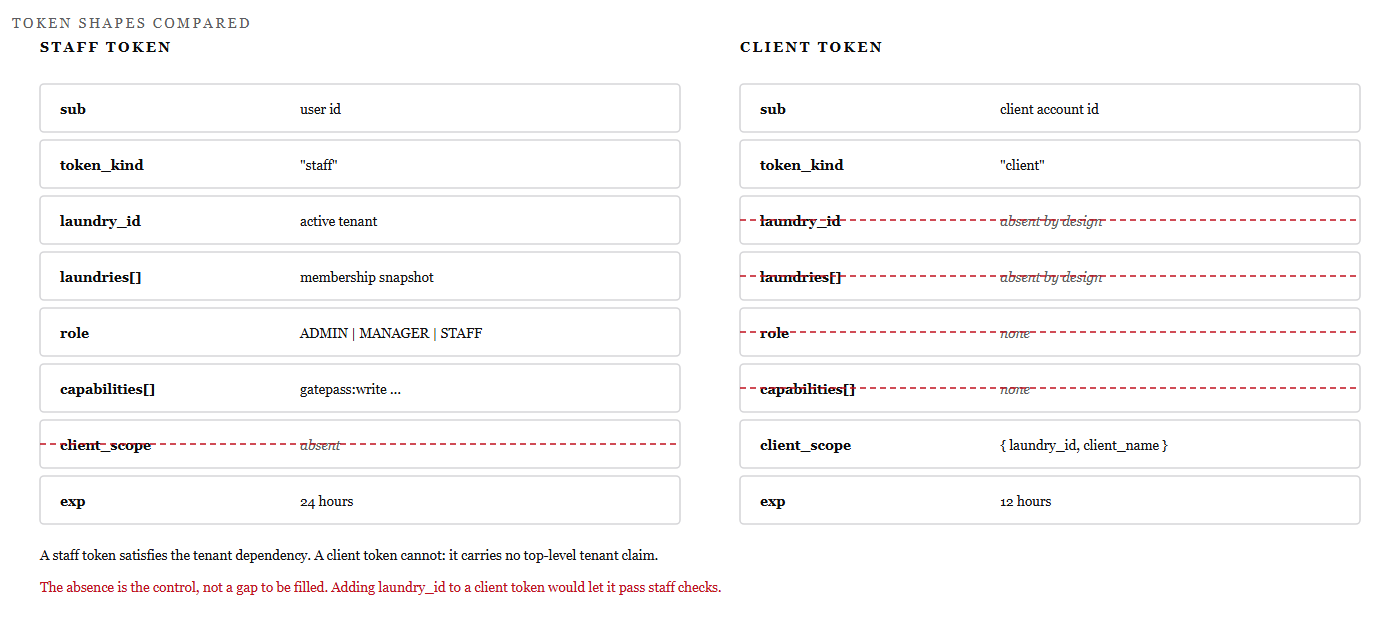
\includegraphics[width=\linewidth]{images/fig-09.png}
\caption{— Claim-by-claim comparison of staff and hotel client tokens.Figure 9}
\end{figure}
The two tokens are not variants of one design; they are different instruments. A staff token asserts a person, a tenant and a set of capabilities. A client token asserts a property and a scope, and nothing else — no tenant claim, no role, no capability list.

The asymmetry is what makes the isolation automatic. Staff endpoints resolve a tenant from the token, so a token without one cannot pass, no matter which route it is sent to. Hotel endpoints read the scope object, so a staff token cannot satisfy them either.

\begin{notebox}RuleAdding a tenant claim to a client token to simplify a query would collapse the distinction and let a hotel satisfy a staff authorisation check. The absence is the control.\end{notebox}
\part{The Applications}
\textsc{\small\color{crimson}Part Two · User Manual — Laundry App}\par\medskip
\chapter{User Manual — Laundry App}
\begin{quote}\itshape The full-surface application for the laundry business: passes, deliveries, bills, quotations, workers, reports and day close.\end{quote}
\section{4.1 Sign-in}
The laundry app is the quotations-ui application, extended for the operational modules. It is the only surface that exposes the complete commercial picture, and therefore the only one where a manager can move from a gate pass to the bill it produced and the payment that settled it.

\begin{figure}[htbp]
\centering
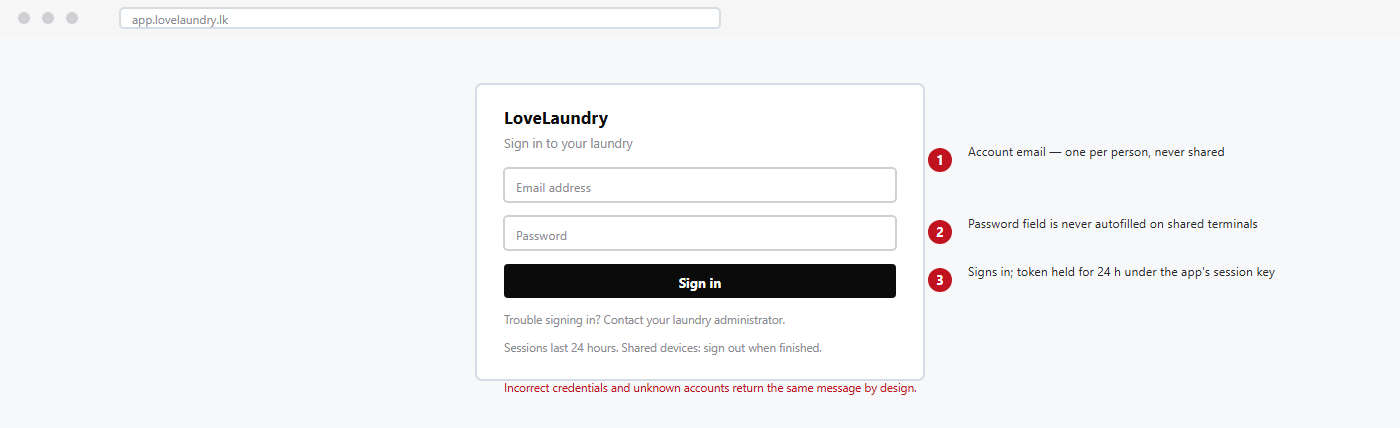
\includegraphics[width=\linewidth]{images/fig-10.png}
\caption{— Laundry app sign-in with field annotations.Figure 10}
\end{figure}
\subsubsection*{Procedure — signing in}
4 · User Manual — Laundry AppLoveLaundry — System Manual

\begin{enumerate}
\item Open the laundry app in a supported browser on a device you control.
\item Enter your account email. Use your own account: the audit trail, and therefore every correction you make, is attributed to it.
\item Enter your password and select .\textbf{Sign in}
\item If you hold memberships in more than one laundry, choose the laundry you are working in for this session. The choice is bound to the session and cannot be changed without signing in again.
\item Confirm the laundry name shown in the top bar matches the business you are working for before entering any data.
\end{enumerate}
\begin{notebox}NoteSign-in failures do not distinguish between a wrong password and an unknown account. This is deliberate: a different message would let an outsider discover which email addresses have accounts.\end{notebox}
\section{4.2 Dashboards}
The dashboard answers one question: what needs attention today? It is not a reporting surface — reports live under  — and it is not a workflow queue. Every tile is either a count that should be driven to zero, or a total that should match a physical count.\textbf{Reports}

\begin{center}\small
\begin{tabularx}{\linewidth}{|X|X|}
\hline
\rowcolor{lightgrey}
\textbf{Tile} & \textbf{Meaning and expected action} \\ \hline
Open gate passes & Passes received but not yet fully delivered. A number that only grows means deliveries are not being recorded, not that work is piling up. \\ \hline
Due today & Passes whose promised return date is today. Work these first; the tile turns amber when any item is overdue. \\ \hline
Ready for delivery & Items washed, pressed and marked ready in the linen room. These are physically on the rack and should leave today. \\ \hline
Unbilled deliveries & Deliveries recorded but not yet included in a bill. The figure should be zero at day close; anything left is revenue at risk. \\ \hline
Outstanding balance & Sum of unpaid balances across clients for the current period. Drill through to the client list, then to the bill. \\ \hline
Linen discrepancies & Open missing or damaged records. These need a supervisor decision, not a silent write-off. \\ \hline
Today's collections & Payments posted today, split by method. Compare with the cash drawer and the bank slip before day close. \\ \hline
\end{tabularx}
\end{center}
\subsection*{Reading the dashboard honestly}
Tiles are computed from the operational database on request; they are not maintained counters. That means they are always consistent with the documents behind them, and it also means a tile can change while you are looking at it if a colleague records a delivery. There is no stale cache to reason about, and no nightly job that could leave a number wrong until morning.

Each tile is a link. A count without a route to the underlying records is a number nobody can act on, so every tile opens a filtered list — open passes, due-today passes, unbilled deliveries — with the filter already applied and visible in the toolbar.

4 · User Manual — Laundry AppLoveLaundry — System Manual

\subsubsection*{Daily rhythm}
\begin{center}\small
\begin{tabularx}{\linewidth}{|X|X|X|}
\hline
\rowcolor{lightgrey}
\textbf{When} & \textbf{Look at} & \textbf{Why} \\ \hline
Opening & Due today, ready for delivery & Plan the routes and the wash order before the first van leaves. \\ \hline
Midday & Open passes, linen discrepancies & Catch missing items while the shift that handled them is still on site. \\ \hline
Before dispatch & Ready for delivery, due today & Confirm that what is on the rack matches what the client expects. \\ \hline
Evening & Unbilled deliveries, outstanding balance & Raise missing bills and chase balances before day close. \\ \hline
Day close & Today's collections & Reconcile cash and card totals against the drawer. \\ \hline
\end{tabularx}
\end{center}
\begin{notebox}WarningA dashboard that shows zero unbilled deliveries at the end of the day is only meaningful if every delivery was recorded as it happened. Recording a week of deliveries retrospectively makes the figures look correct while destroying their value for decisions.\end{notebox}
\section{4.3 Gate passes}
The gate-pass register is the operational spine of the laundry. Every collection is recorded here, every delivery refers back to a pass, and every bill is built from delivered quantities. A pass records who sent what, when it arrived and when it is promised back.

\begin{figure}[htbp]
\centering
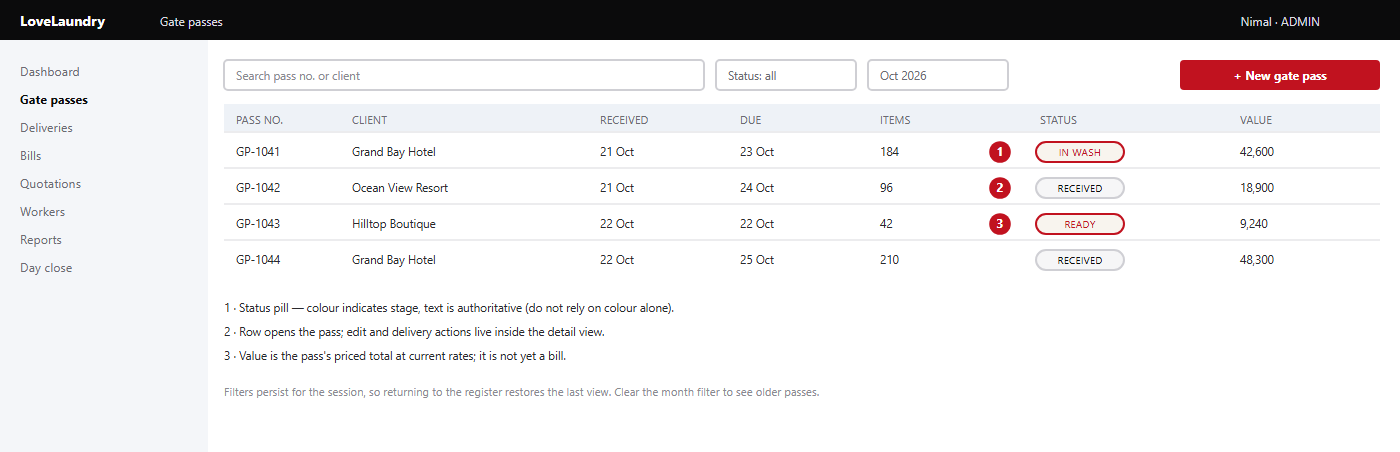
\includegraphics[width=\linewidth]{images/fig-11.png}
\caption{— Gate-pass register with annotations.Figure 11}
\end{figure}
\subsubsection*{Columns and statuses}
The register shows the pass number, the client, the date received, the promised return date, the item count and the current status. Statuses advance only through recorded actions:  when the pass is created,  when the linen room starts processing,  when finishing is complete,  when a delivery is recorded against it, and  when nothing further is outstanding. A pass is never deleted; a mistake is corrected by cancelling the pass with a reason, which leaves it visible in the register.\emph{received}\emph{in wash}\emph{ready}\emph{delivered}\emph{closed}

\section{4.4 Creating a gate pass}
A gate pass is created at the moment goods are handed over. Doing it later, from memory, is the single largest source of billing disputes, because the quantities recorded then are guesses rather than counts.

4 · User Manual — Laundry AppLoveLaundry — System Manual

\begin{figure}[htbp]
\centering
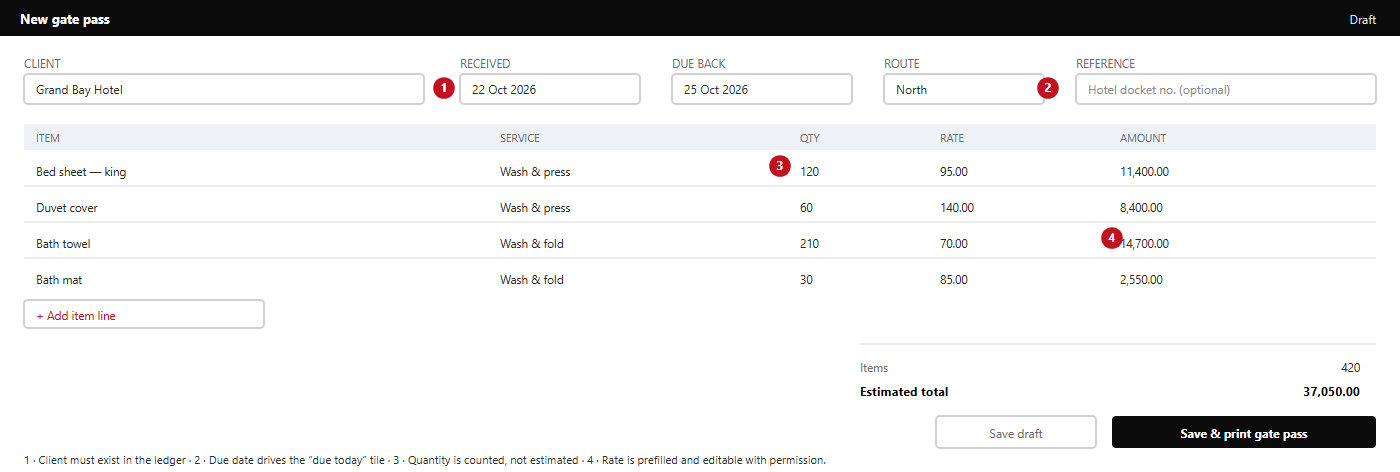
\includegraphics[width=\linewidth]{images/fig-12.png}
\caption{— Gate-pass editor, showing header fields and item lines.Figure 12}
\end{figure}
\subsubsection*{Procedure — creating a gate pass}
\begin{enumerate}
\item From the register, select .\textbf{+ New gate pass}
\item Choose the client. If the client is not listed, stop and ask an administrator to create the client record; do not type a variant of an existing name, which splits the client's history.
\item Set the date received to the actual handover date. Back-dating a pass distorts the monthly matrix and the day-close totals for both dates.
\item Set the promised return date. This is the date the client has been told; it drives the due-today worklist.
\item Add each item line: item, service, quantity and rate. Count the goods as you add them — the pass is a receipt as well as a work order.
\item Check the item count and estimated total against the physical count one more time. A typo here propagates into the delivery and the bill.
\item Select  and hand the printed copy to the client's driver. The pass is now locked for quantity edits except by a manager, and every such edit is audited.\textbf{Save \& print gate pass}
\end{enumerate}
\begin{notebox}WarningNever create a pass for goods that have not arrived. A pass is evidence of possession; creating one early turns a missing delivery into a billing dispute.\end{notebox}
\section{4.5 Deliveries}
A delivery records the return of finished goods against a gate pass. It is the bridge between operations and money: quantities delivered are what the client is billed for, and the delivery date determines the billing period.

\subsection*{Partial and split deliveries}
Clients rarely receive a whole pass at once. A hotel may take back its sheets today and its towels tomorrow, and the platform expects this. Each delivery carries its own quantities per line, and the pass remains open until the delivered quantity equals the received quantity on every line, or until a supervisor closes the balance as short-delivered with a reason.

4 · User Manual — Laundry AppLoveLaundry — System Manual

\begin{center}\small
\begin{tabularx}{\linewidth}{|X|X|}
\hline
\rowcolor{lightgrey}
\textbf{Situation} & \textbf{What the system does} \\ \hline
Delivered < received & Pass stays open; remaining quantity is shown as outstanding on the pass and in the due-today tile. \\ \hline
Delivered = received & Pass status becomes delivered; the lines become billable. \\ \hline
Delivered > received & Rejected. An over-delivery means either the pass quantity or the delivery count is wrong; correct the record rather than forcing the number. \\ \hline
Short delivery closed & Requires a reason and a supervisor. The undelivered quantity is written off explicitly and appears in the discrepancy report. \\ \hline
Delivery corrected after billing & Requires a credit note; the original delivery is not edited once a bill has consumed it. \\ \hline
\end{tabularx}
\end{center}
\subsubsection*{Procedure — recording a delivery}
\begin{enumerate}
\item Open  and select , or open the pass and choose  from its detail view.\textbf{Deliveries}\textbf{Record delivery}\textbf{Deliver}
\item Scan or select the gate pass. The form loads every line with the outstanding quantity prefilled.
\item Reduce quantities to what is actually being handed over. Leave a line at zero if nothing on it is going out.
\item Confirm the receiver's name — the person signing at the client — and the delivery date and time.
\item Select . The pass status recalculates immediately and the dashboard tiles update.\textbf{Save delivery}
\item Print or share the delivery note if the client requires one. The note shows quantities only, never rates.
\end{enumerate}
\subsection*{What a delivery is not}
\begin{itemize}
\item Delivering goods does not raise an invoice. Bills are raised deliberately, in a batch or per client, so that the billing period is a business decision rather than a side effect of a van leaving.\textbf{Not a bill.}
\item A delivery can be made on credit. The balance appears on the bill, and payment is a separate record with its own audit trail.\textbf{Not a payment.}
\item A delivery recorded in error is reversed with a reason, which leaves both records visible. Deleting one would hide the fact that goods may have left the premises.\textbf{Not reversible by deletion.}
\end{itemize}
\begin{notebox}NoteThe receiver's name matters more than it appears to. When a hotel later disputes a delivery, the name and timestamp on the note are the evidence that resolves it — which is why the field is required and is not defaulted to the signed-in user.\end{notebox}
\section{4.6 Bills}
A bill is raised against a client for deliveries in a period. It states quantities, rates, charges, discounts and tax, and it carries the balance outstanding. Bills are the platform's commercial record: once issued, a bill is not edited, because an edited invoice cannot be reconciled against the copy the client holds.

\subsubsection*{Raising a bill}
4 · User Manual — Laundry AppLoveLaundry — System Manual

\begin{enumerate}
\item Open  and select .\textbf{Bills}\textbf{Raise bill}
\item Choose the client and the period. The form lists every unbilled delivery for that client in the period, with its pass reference.
\item Select the deliveries to include. Deliveries already on another bill are not offered, which prevents double billing at the source.
\item Review the line rates. Rates come from the client's agreed price list where one exists; a manual override requires  and is visible on the bill as an edited rate.\texttt{bill:write}
\item Apply any discount or adjustment with a reason. A discount without a reason is a control failure, not a courtesy.
\item Check the totals: subtotal, discount, tax and amount due. Tax is computed from the configured rate, not typed.
\item Select . The bill receives its number, becomes immutable, and the client's balance increases.\textbf{Issue bill}
\item Print or share the bill. The print layout is produced by the guest-billing view, which shows the same figures as the screen.
\end{enumerate}
\begin{center}\small
\begin{tabularx}{\linewidth}{|X|X|}
\hline
\rowcolor{lightgrey}
\textbf{Attribute} & \textbf{Rule} \\ \hline
Number & Assigned on issue, sequential within the laundry and the financial year. Numbers are never reused, including for cancelled bills. \\ \hline
Status & before issue,  after,  or  as payments arrive,  if cancelled with a reason.\emph{draft}\emph{issued}\emph{part-paid}\emph{paid}\emph{void} \\ \hline
Immutability & Issued bills do not change. Corrections are credit notes or adjustment records that reference the original. \\ \hline
Currency & One currency per laundry, set in configuration; bills do not convert. \\ \hline
\end{tabularx}
\end{center}
\subsection*{Draft, issue, and the point of no return}
A draft bill can be edited freely — lines added, rates corrected, the period changed. Issuing it is the point at which it becomes a financial document: the number is consumed, the client can see it in the hotel portal if they have an account, and any correction must be made by a visible adjustment rather than an edit. Staff who are unsure whether a bill is right should leave it in draft; a draft is invisible to the client, and nothing is lost by waiting.

\subsection*{What goes on a bill}
\begin{itemize}
\item Only delivered quantities. Work in progress is not billable, however far advanced it is.
\item Rates that were agreed for that client, at the version in force on the delivery date.
\item Adjustments from returns or short deliveries, shown as separate lines rather than netted silently into quantities.
\item Tax computed by the platform from configuration, with the rate stated on the face of the bill.
\end{itemize}
\begin{notebox}WarningIf a bill total looks wrong after issue, do not edit the bill. Raise a credit note or an additional charge and reference the original. Editing an issued bill breaks the client's copy, the statement and the audit trail at once.\end{notebox}
4 · User Manual — Laundry AppLoveLaundry — System Manual

\textsc{\small\color{crimson}4.7 · Bill detail and payments}\par\medskip
\section*{Bill detail and payments}
A bill's detail view is the client's account in miniature: what was billed, what has been paid, what remains, and every document that produced those figures. Payments recorded here are the only way a balance falls.

\begin{center}\small
\begin{tabularx}{\linewidth}{|X|X|X|}
\hline
\rowcolor{lightgrey}
\textbf{Method} & \textbf{Recorded as} & \textbf{Effect on balance} \\ \hline
Cash & Receipt against the bill, with drawer reference & Reduces balance immediately \\ \hline
Card & Receipt with terminal reference & Reduces balance on posting; settlement is a banking matter \\ \hline
Bank transfer & Receipt with transfer reference & Reduces balance when posted, not when the bank clears \\ \hline
Cheque & Receipt with cheque number and bank & Reduces balance on posting; bounced cheques are reversed \\ \hline
Credit adjustment & Adjustment record with reason & Reduces balance without cash; audited separately \\ \hline
\end{tabularx}
\end{center}
\subsubsection*{Procedure — recording a payment}
\begin{enumerate}
\item Open the bill from  or from the client's account view.\textbf{Bills}
\item Select . The amount due is prefilled; overwrite it for a part payment.\textbf{Record payment}
\item Choose the method and enter the reference — drawer slip, terminal slip or transfer reference. A payment without a reference cannot be reconciled at day close.
\item Set the payment date to the date the money was received, not the date it was entered.
\item Select . The balance recalculates and the bill status moves to part-paid or paid.\textbf{Post payment}
\item Print the receipt if the client is present, and file the slip with the day's takings.
\end{enumerate}
\subsubsection*{Reversals, not deletions}
A payment posted in error is reversed, never deleted. The reversal creates a negative record that references the original, so the client's statement shows both the mistake and its correction. Deleting a payment would make the day-close total disagree with the bank without explanation — the classic symptom that turns a five-minute correction into an audit.

\begin{notebox}WarningApplying a payment to the wrong bill is corrected by reversing it and re-posting to the correct bill. Never edit the original amount: the receipt the client holds would no longer match the record.\end{notebox}
\textsc{\small\color{crimson}4.8 · Quotations}\par\medskip
\section*{Quotations}
A quotation is a priced offer. It carries line items, rates, validity and terms, and it can be converted into operational work — but it never becomes a bill by itself. The separation matters: a quotation is a promise about price, while a bill is a statement of work actually delivered.

4 · User Manual — Laundry AppLoveLaundry — System Manual

\begin{center}\small
\begin{tabularx}{\linewidth}{|X|X|X|}
\hline
\rowcolor{lightgrey}
\textbf{State} & \textbf{Meaning} & \textbf{Allowed next steps} \\ \hline
draft & Being prepared; not visible to the client & Edit, send, discard \\ \hline
sent & Issued to the client with a validity date & Accept, decline, expire, revise \\ \hline
accepted & Client has agreed the price & Convert to gate pass or client rate card \\ \hline
declined & Client rejected the offer & Revise as a new draft \\ \hline
expired & Validity date passed without a decision & Re-issue with a new validity date \\ \hline
\end{tabularx}
\end{center}
\subsubsection*{Procedure — preparing a quotation}
\begin{enumerate}
\item Select  and choose the prospective or existing client.\textbf{Quotations → New quotation}
\item Add line items: item, service, quantity and rate. Use the item catalogue where possible so that the wording matches the eventual bill.
\item Set the validity period. A quotation without an end date is a price the laundry may be held to indefinitely.
\item Review the totals and any terms, then select  or  once the client has received it.\textbf{Send}\textbf{Mark as sent}
\item When the client accepts, record the acceptance and convert the quotation. Conversion creates a draft gate pass or updates the client's rate card; it does not create a bill.
\end{enumerate}
\subsubsection*{AI assistance}
The quotation module can draft line items and wording through the AI chat surface. Drafts are suggestions: every rate and quantity must be reviewed before the quotation is sent, and the platform records who issued it, not what suggested it. The assistant has no ability to send a quotation or to change a price without a user action.

\begin{notebox}NoteA converted quotation is linked to its source. When a client later disputes a rate, the chain from quotation to pass to bill is visible in one place.\end{notebox}
\textsc{\small\color{crimson}4.9 · Workers}\par\medskip
\section*{Workers}
The worker register records the people who do the work and, where the laundry pays by output, the work attributed to them. It is deliberately simple: identity, role, status and assignment. Payroll arithmetic belongs to the accounting service, not to the operational record.

\begin{center}\small
\begin{tabularx}{\linewidth}{|X|X|X|}
\hline
\rowcolor{lightgrey}
\textbf{Field} & \textbf{Purpose} & \textbf{Notes} \\ \hline
Worker code & Short identifier used on production sheets & Unique within the laundry \\ \hline
Name & Display name on assignment lists & Editable; historical records keep the name at the time \\ \hline
Role & Washer, presser, driver, checker, supervisor & Drives which worklists the worker appears in \\ \hline
Status & Active, on leave, inactive & Inactive workers cannot be assigned new work \\ \hline
Contact & Phone for shift coordination & Optional; treated as personal data \\ \hline
\end{tabularx}
\end{center}
4 · User Manual — Laundry AppLoveLaundry — System Manual

\subsubsection*{Procedure — adding a worker}
\begin{enumerate}
\item Open  and select .\textbf{Workers}\textbf{Add worker}
\item Enter the worker code exactly as it appears on the laundry's own records; the code is how production sheets are reconciled.
\item Set the role and status. A worker who has left is set to inactive rather than deleted, because historic assignments reference them.
\item Save. The worker appears in assignment lists for the roles selected.
\end{enumerate}
\subsubsection*{Assignment and accountability}
Work can be attributed to a worker at the gate-pass level, the item-line level, or at the wash batch level in the linen room. Attribution is optional for operations and essential for piece-rate payroll: if a laundry pays by item, the assignment is the evidence of who processed what. Where attribution is used, it must be recorded at the time of work, not reconstructed at the end of the week.

\begin{notebox}NoteAttendance and salary records live in laundry-management, not here. The worker register supplies identity to both, so a name change in one place does not silently diverge from the other.\end{notebox}
\textsc{\small\color{crimson}4.10 · Reports and the monthly matrix}\par\medskip
\section*{Reports and the monthly matrix}
Reports answer questions that outlive the day. They are computed from the same operational documents as the dashboards, so a report never disagrees with the screen it summarises — and a report is only as good as the discipline with which passes and deliveries were recorded.

\begin{center}\small
\begin{tabularx}{\linewidth}{|X|X|X|}
\hline
\rowcolor{lightgrey}
\textbf{Report} & \textbf{Answers} & \textbf{Typical use} \\ \hline
Daily production & What was received, washed and delivered on a date & Shift handover and capacity planning \\ \hline
Client statement & Every bill, payment and balance for one client & Month-end credit control \\ \hline
Monthly matrix & Quantities and values by client by day & Contract reconciliation and volume checks \\ \hline
Unbilled deliveries & Delivered work not yet on a bill & Revenue at risk before day close \\ \hline
Linen discrepancy & Missing, damaged and short-delivered items & Loss investigation and client conversations \\ \hline
Worker productivity & Items or batches attributed per worker & Piece-rate payroll and scheduling \\ \hline
\end{tabularx}
\end{center}
\subsubsection*{The monthly matrix}
The matrix is a grid: clients down the side, days of the month across the top, and a cell for each day holding the quantity and value processed for that client. It exists because a monthly total hides the pattern that matters — a client whose volume collapses for four days, or a day on which one client's items were entered against another's name.

4 · User Manual — Laundry AppLoveLaundry — System Manual

Rows are clients, columns are calendar days, and the final columns total the month. Cells are derived from gate passes (received) and deliveries (returned), so the matrix is a view, not a ledger: nothing is typed into it, and it cannot be edited. A cell that looks wrong is a pass that was entered wrongly, and that is where the correction belongs.

\begin{notebox}NoteExport the matrix before a contract review. It is the document clients recognise, and it is generated from the same records that produced their bills.\end{notebox}
\textsc{\small\color{crimson}4.11 · Day close}\par\medskip
\section*{Day close}
Day close is the point at which a business date stops moving. It freezes the day's totals, confirms that every delivery has been billed or consciously deferred, and records who closed the day and when. It is a control, not a formality: most reconciliation failures are discovered at close, which is exactly when they are cheapest to fix.

\subsubsection*{Procedure — closing the day}
\begin{enumerate}
\item Confirm that all gate passes for the date are recorded. Compare the register with the paper collection book.
\item Confirm that all deliveries made today are recorded and that no pass is left open without a reason.
\item Check . Raise the missing bills, or record why a delivery is intentionally held into the next period.\textbf{Unbilled deliveries}
\item Reconcile  against the cash drawer and the card terminal report. Record any difference with an explanation.\textbf{Today's collections}
\item Review linen discrepancies raised during the day and confirm that each has an owner.
\item Select . The system writes a day-close record with totals, the operator and a timestamp.\textbf{Close day}
\item Print or save the close summary and attach it to the day's banking.
\end{enumerate}
\begin{center}\small
\begin{tabularx}{\linewidth}{|X|X|}
\hline
\rowcolor{lightgrey}
\textbf{Item} & \textbf{Effect of closing} \\ \hline
Bill totals & Figures for the date become the reported figures; later corrections appear on the date they are made \\ \hline
Payment totals & Collections for the date are fixed for reconciliation \\ \hline
Delivery counts & Volumes reported in the monthly matrix stop changing for that day \\ \hline
Day-close record & Immutable; a correction requires a reopening with a reason \\ \hline
\end{tabularx}
\end{center}
\begin{notebox}WarningDo not close a day to make a warning disappear. A closed day with an unresolved discrepancy is harder to correct than an open one, because reopening is itself an audited event.\end{notebox}
4 · User Manual — Laundry AppLoveLaundry — System Manual

\textsc{\small\color{crimson}4.12 · Administration, users and common errors}\par\medskip
\section*{Administration, users and common errors}
Administration in the laundry app is limited to the tenant you are signed in to: users, their memberships and roles, and hotel client accounts for your own clients. Creating a laundry is a platform operation, described in Chapter 8.1, and is not available from this application.

\subsubsection*{Users and roles}
A user is a person with a login. A membership is that person's link to your laundry, carrying their role. Removing someone's access means removing the membership, not deleting the user — they may belong to another laundry, and their history on your records must remain attributable.

\begin{center}\small
\begin{tabularx}{\linewidth}{|X|X|X|}
\hline
\rowcolor{lightgrey}
\textbf{Message or symptom} & \textbf{Usual cause} & \textbf{Action} \\ \hline
403 — tenant could not be resolved & Token issued without a tenant, or a client token used on a staff route & Sign out and sign in again; hotel accounts must use the Hotel Desk app \\ \hline
403 — capability required & Role lacks the capability for this action & Ask an administrator to review the membership role \\ \hline
409 — duplicate pass number & Two passes created from the same paper docket & Open both, keep the correct one, cancel the other with a reason \\ \hline
422 — quantity exceeds received & Delivery quantity larger than the pass line & Recount; correct the pass quantity with a manager if the pass was wrong \\ \hline
Bill total differs from the print & Bill edited after issue, or printed from a stale tab & Reload the bill; issued bills cannot change, so a difference indicates a stale view \\ \hline
Dashboard tile shows zero & Filter applied, or the day is closed & Clear the date filter; check the day-close record \\ \hline
\end{tabularx}
\end{center}
\begin{notebox}NoteErrors that mention a capability or a tenant are authorisation outcomes, not faults. Report the exact message to an administrator; it names what was missing.\end{notebox}
\textsc{\small\color{crimson}4.13 · Day-close sequence}\par\medskip
\section*{Day-close sequence}
What has to be true before a date can be frozen, and what happens when it is not.

4 · User Manual — Laundry AppLoveLaundry — System Manual

\begin{figure}[htbp]
\centering
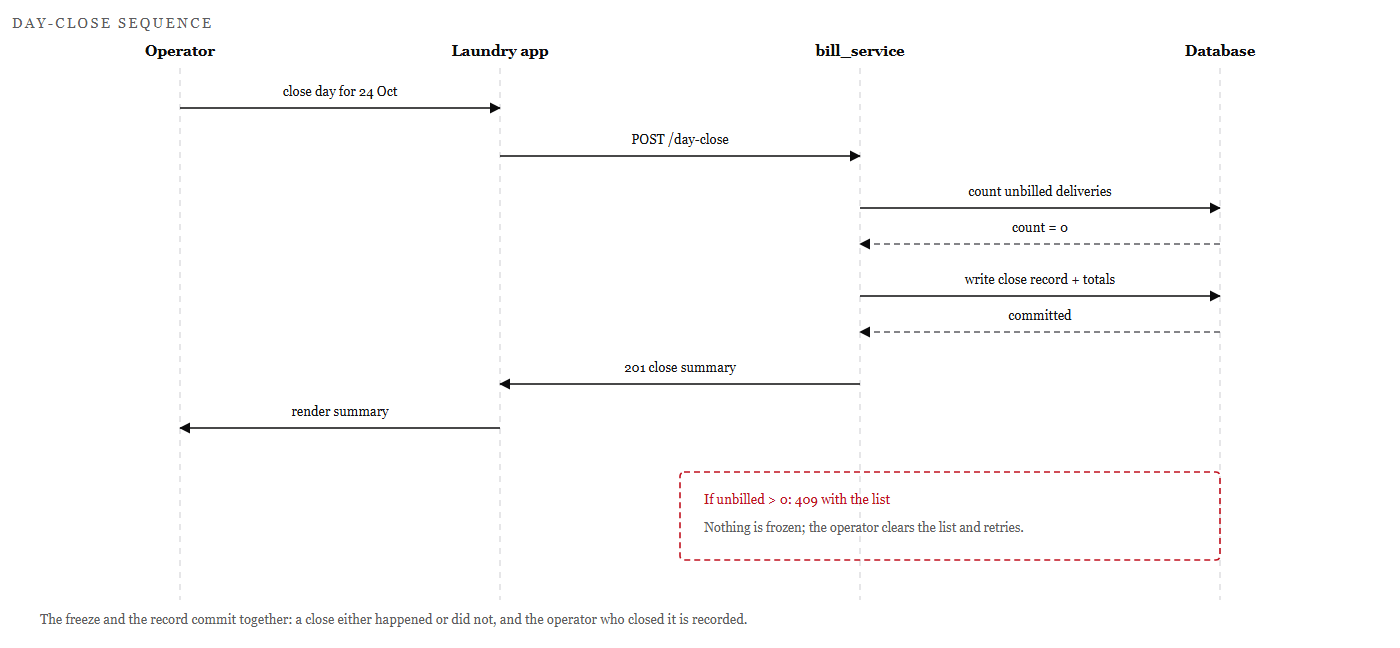
\includegraphics[width=\linewidth]{images/fig-13.png}
\caption{— Day-close sequence, including the blocked branch when unbilled deliveries remain.Figure 13}
\end{figure}
Closing a day is a transaction with a precondition, not a button that writes a total. The service counts unbilled deliveries first; if any exist, it refuses and returns the list. Nothing is frozen, so the operator can correct the cause and try again.

When the close succeeds, the totals and the close record commit together. That single unit is what makes the day's figures defensible: there is no state in which a date is marked closed but its totals were never written.

\begin{notebox}RuleA close that fails is cheaper than a close that succeeds with an unresolved discrepancy. Reopening is itself an audited event and is never the first resort.\end{notebox}
\textsc{\small\color{crimson}Part Two · User Manual — Shop Counter App}\par\medskip
\chapter{User Manual — Shop Counter App}
\begin{quote}\itshape A point-of-sale surface for walk-in customers: fast, narrow, and reconciled at the end of every shift.\end{quote}
\section{5.1 Overview and sign-in}
The Shop Counter app is the shop-app front end. It serves a different transaction from the laundry: a customer arrives with a bag, not an account, and leaves with a receipt. Everything about the interface follows from that: few required fields, large targets, keyboard-first entry, and a day close that reconciles takings rather than work in progress.

\begin{center}\small
\begin{tabularx}{\linewidth}{|X|X|}
\hline
\rowcolor{lightgrey}
\textbf{Attribute} & \textbf{Value} \\ \hline
Application & shop-app — React 19, TypeScript, Vite 8, Tailwind 4 \\ \hline
Development port & 5174 \\ \hline
Sign-in endpoint & POST /auth/login (user-service) \\ \hline
Session key & ll\_shop\_session \\ \hline
Core records & Shop bills, today's takings, day-close totals \\ \hline
Typical user & Counter staff, shop supervisor \\ \hline
\end{tabularx}
\end{center}
5 · User Manual — Shop Counter AppLoveLaundry — System Manual

\subsubsection*{Procedure — signing in at the counter}
\begin{enumerate}
\item Open the Shop Counter app on the counter terminal.
\item Enter your own staff email and password, then select .\textbf{Sign in}
\item Confirm the laundry name in the header is your shop, and that the date shown is today.
\item Leave the session open for the shift. The token lasts 24 hours, but a shared terminal should be signed out at handover.
\end{enumerate}
\begin{notebox}WarningNever sign in with a colleague's account to “save time”. Every void, refund and discount is attributed to the signed-in user, and a shared login makes those actions unattributable.\end{notebox}
\textsc{\small\color{crimson}5.2 · Today view}\par\medskip
\section*{Today view}
The today view is the shop's home screen and, for most staff, the only screen they need between customers. It answers three questions: what have I taken today, what is waiting to be finished, and what did the last few transactions look like?

\begin{figure}[htbp]
\centering
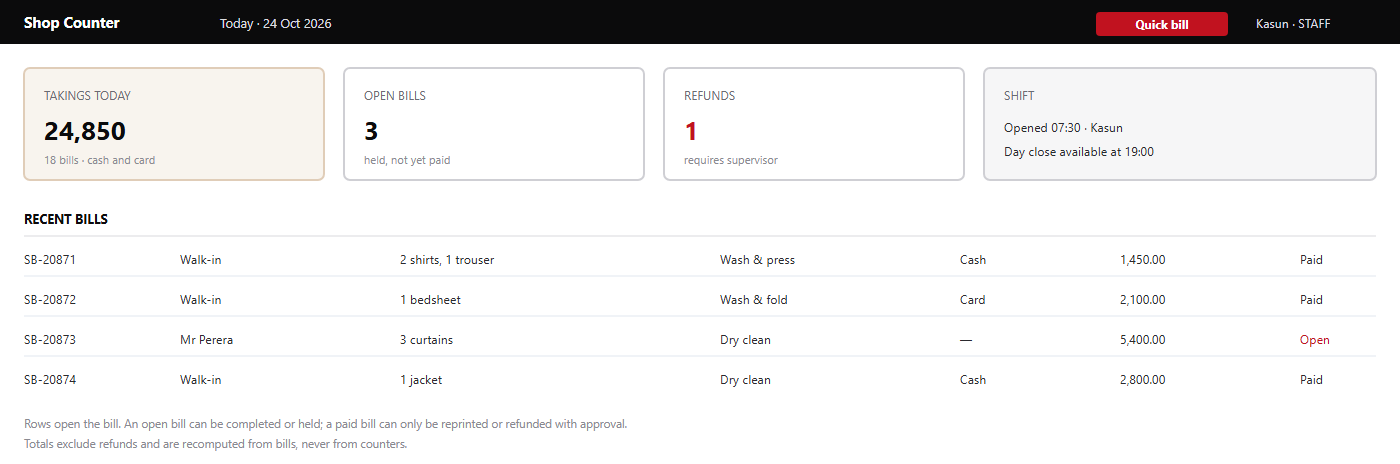
\includegraphics[width=\linewidth]{images/fig-14.png}
\caption{— Shop Counter today view.Figure 14}
\end{figure}
\subsubsection*{What the tiles mean}
is the sum of paid shop bills for the business date, split by tender in the detail.  are transactions started but not settled — held garments awaiting collection, or a bill left open while the customer finds a card.  counts refunds recorded today and flags that each requires supervisor approval. The  panel names who opened the till and when day close becomes available.\textbf{Takings today}\textbf{Open bills}\textbf{Refunds}\textbf{shift}

\begin{notebox}WarningA large open-bill count at closing time usually means bills were abandoned mid-transaction rather than held deliberately. Resolve them before day close; an abandoned bill is a customer who left without paying and without a receipt.\end{notebox}
5 · User Manual — Shop Counter AppLoveLaundry — System Manual

\textsc{\small\color{crimson}5.3 · Bills}\par\medskip
\section*{Shop bills}
Shop bills are counter sales. They carry their own numbering, separate from laundry bills, because they are a different kind of document: a completed retail transaction rather than a periodic charge for work done. Keeping them separate means shop takings reconcile cleanly and laundry receivables are not diluted by walk-in cash.

\begin{center}\small
\begin{tabularx}{\linewidth}{|X|X|X|}
\hline
\rowcolor{lightgrey}
\textbf{State} & \textbf{Meaning} & \textbf{What is still possible} \\ \hline
draft & Items added, not yet taken to payment & Edit lines, apply discount, abandon \\ \hline
open & Payment not completed; customer may return & Complete payment, hold, add items \\ \hline
paid & Tendered and receipted & Reprint, refund with approval \\ \hline
refunded & Fully reversed after payment & None; a new bill is required for new goods \\ \hline
void & Cancelled before payment, with a reason & None; the number is retained \\ \hline
\end{tabularx}
\end{center}
\subsubsection*{Procedure — completing a sale}
\begin{enumerate}
\item Select , or open an existing draft bill.\textbf{Quick bill}
\item Add items: choose from the catalogue or type a free line where the catalogue has no entry.
\item Confirm quantities and rates aloud with the customer before taking payment.
\item Select the tender: cash or card. For cash, enter the amount tendered so the change is calculated and shown.
\item Select . The bill moves to paid and the receipt is offered for printing.\textbf{Take payment}
\item Hand over the receipt and the goods together. The receipt is the customer's evidence of the transaction and the shop's evidence of the tender.
\end{enumerate}
\subsubsection*{Discounts and their limits}
A discount is a line-level or bill-level reduction with a reason. Counter staff may apply the configured standard discount; anything beyond it requires a supervisor, and the reason is recorded against the bill. The point is not to prevent generosity but to make it visible: a discount without a reason is indistinguishable from an error, and at month end it is indistinguishable from theft.

\begin{notebox}NoteVoided and refunded bills keep their numbers. Reconciling a day's takings against a bill sequence with gaps is far harder than reconciling one where every number is accounted for.\end{notebox}
\textsc{\small\color{crimson}5.4 · Quick bill}\par\medskip
\section*{Quick bill}
Quick bill is the counter's fast path: a numeric keypad, the most-used services as one-touch buttons, and a single total. It exists because the difference between a twelve-second and a forty-second transaction is the difference between a queue and a complaint.

5 · User Manual — Shop Counter AppLoveLaundry — System Manual

\begin{figure}[htbp]
\centering
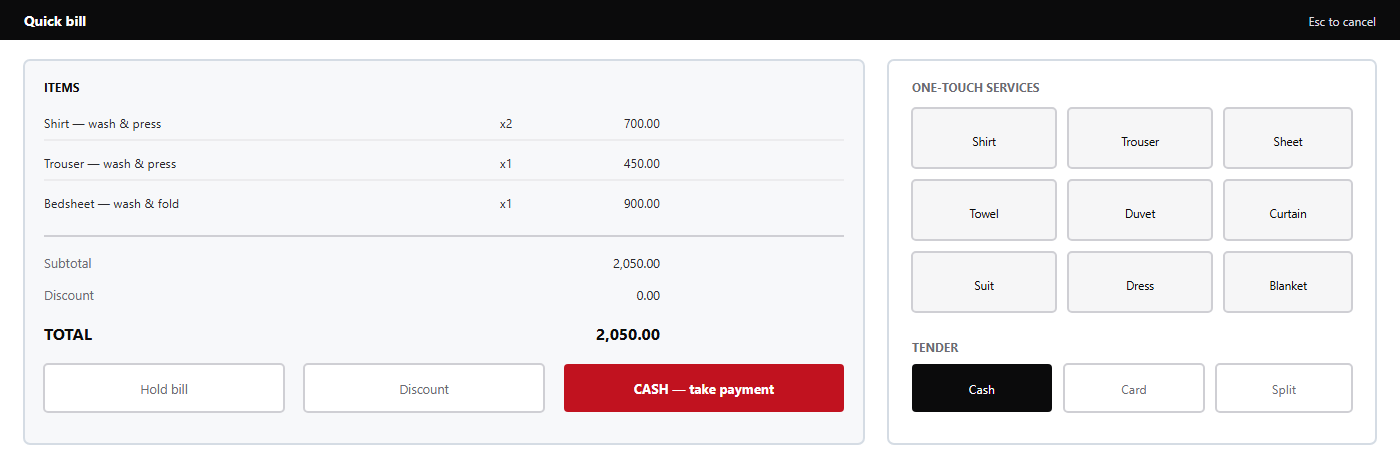
\includegraphics[width=\linewidth]{images/fig-15.png}
\caption{— Quick bill pad: item list left, one-touch services and tender right.Figure 15}
\end{figure}
\subsubsection*{Procedure — a cash sale in under a minute}
\begin{enumerate}
\item Select  from the header.\textbf{Quick bill}
\item Tap the service buttons for each garment type; adjust quantity with the keypad if more than one.
\item Read the total to the customer and confirm the item count.
\item Select , enter the amount tendered, and confirm the change shown.\textbf{Cash}
\item Print the receipt. The bill is now paid and appears in today's takings.
\end{enumerate}
Card sales follow the same path with the  tender; the terminal is separate, and the app records the reference so the day close can be reconciled against the terminal report. Split tender is used when a customer pays part cash and part card, and the app requires both amounts to sum to the total before it will accept the payment.\textbf{Card}

\begin{notebox}NoteQuick bill never creates a laundry bill, a gate pass or a linen record. If a customer wants laundry service rather than a counter sale, use the laundry app.\end{notebox}
\textsc{\small\color{crimson}5.5 · Day close}\par\medskip
\section*{Day close at the counter}
The shop's day close is shorter than the laundry's, and it has one job: prove that the money in the drawer matches the money recorded. Everything else — bills raised, refunds given, discounts applied — is detail that explains a difference, not a difference itself.

\subsubsection*{Procedure — closing the shop day}
5 · User Manual — Shop Counter AppLoveLaundry — System Manual

\begin{enumerate}
\item Resolve every open bill: complete payment, or void it with a reason.
\item Count the drawer and record the counted amount in the close form.
\item Compare the counted amount with the system's cash total. If they differ, enter the difference and a short explanation before closing.
\item Check that card takings match the terminal's end-of-day report.
\item Review refunds and discounts recorded during the shift; each must have an approver.
\item Select . The close record is written with totals, the operator and a timestamp.\textbf{Close day}
\item Print the close summary, attach the terminal report and the bank slip, and hand both to the supervisor.
\end{enumerate}
\begin{center}\small
\begin{tabularx}{\linewidth}{|X|X|X|}
\hline
\rowcolor{lightgrey}
\textbf{Item} & \textbf{Source of truth} & \textbf{Tolerance} \\ \hline
Cash takings & Physical drawer count & Any difference is recorded, not adjusted away \\ \hline
Card takings & Terminal end-of-day report & Must match to the cent; a mismatch is investigated before close \\ \hline
Refunds & Refund records with approver & Each must be approved; unapproved refunds block close \\ \hline
Open bills & Bill list filtered to open & Must be zero, or explicitly held with a reason \\ \hline
\end{tabularx}
\end{center}
\begin{notebox}WarningClosing the day does not move money. If the drawer is short, record the shortage and escalate; do not take cash from a later sale to balance the day.\end{notebox}
\textsc{\small\color{crimson}5.6 · Roles and permissions}\par\medskip
\section*{Roles and permissions at the counter}
The shop uses the same staff roles as the rest of the platform, with capabilities scoped to counter work. A shop user is a member of the laundry with a role; there is no separate shop-only account type. That keeps one identity per person across the business and one audit trail.

\begin{center}\small
\begin{tabularx}{\linewidth}{|X|X|X|}
\hline
\rowcolor{lightgrey}
\textbf{Role} & \textbf{Can do} & \textbf{Cannot do} \\ \hline
STAFF & Create quick bills, complete payment, reprint receipts, hold bills & Give refunds, exceed standard discount, close day, void a paid bill \\ \hline
MANAGER & All counter actions, refunds, discounts beyond standard, day close, reprint any bill & Change user roles, alter shop configuration \\ \hline
ADMIN & Everything a manager can, plus user and membership management for the laundry & Create laundries or act outside the tenant \\ \hline
\end{tabularx}
\end{center}
\subsubsection*{How the controls appear}
The app hides actions the signed-in user cannot perform, so a counter assistant does not see a refund button they are not allowed to use. That is a courtesy, not the control: every action is re-checked on the server against the capability carried in the token. If a hidden action is somehow invoked — a stale tab, a crafted request — it fails with a permission error and an audit entry.

5 · User Manual — Shop Counter AppLoveLaundry — System Manual

\begin{center}\small
\begin{tabularx}{\linewidth}{|X|X|X|}
\hline
\rowcolor{lightgrey}
\textbf{Action} & \textbf{Capability} & \textbf{Held by} \\ \hline
Create or pay a shop bill & bill:write & STAFF, MANAGER, ADMIN \\ \hline
View bills and takings & bill:read & STAFF, MANAGER, ADMIN \\ \hline
Post or reverse a payment & payment:write & MANAGER, ADMIN \\ \hline
View the day-close report & report:read & MANAGER, ADMIN \\ \hline
Open the dashboard & dashboard:read & STAFF, MANAGER, ADMIN \\ \hline
\end{tabularx}
\end{center}
\begin{notebox}NoteA refund is a payment reversal in accounting terms, which is why it needs  and therefore a manager. This is a deliberate restriction, not an oversight.\texttt{payment:write}\end{notebox}
\textsc{\small\color{crimson}5.7 · Procedures}\par\medskip
\section*{Counter procedures}
The four procedures below cover almost every exception a counter encounters. Each is written to be followed under time pressure, with a customer waiting.

\subsubsection*{Procedure — refunding a paid bill}
\begin{enumerate}
\item Open the bill from  or search its number.\textbf{Today}
\item Select . The full amount is prefilled; reduce it for a partial refund.\textbf{Refund}
\item Enter the reason and select the refund tender: cash, or reversal to the original card.
\item Call a supervisor to approve. The approval is recorded against the refund with the approver's name.
\item Hand over the cash or confirm the card reversal, and print the refund slip.
\end{enumerate}
\subsubsection*{Procedure — voiding a bill before payment}
\begin{enumerate}
\item Open the open bill and select .\textbf{Void}
\item Enter the reason: wrong item, customer left, duplicate entry.
\item Confirm. The bill keeps its number and disappears from the open list.
\end{enumerate}
\subsubsection*{Procedure — holding a bill}
Use  when a customer steps away or goes to fetch a card. A held bill stays in the open list with its items intact; it is not a credit sale and it does not reserve stock. At shift handover, resolve every held bill — complete it, void it, or write down why it remains open.\textbf{Hold bill}

\subsubsection*{Procedure — reprinting a receipt}
Open the paid bill and select . The reprint carries the same number and a  marker so that two copies cannot be presented as two transactions. Reprints are audited; a pattern of reprints on the same bill is worth a supervisor's attention.\textbf{Reprint}\emph{duplicate}

5 · User Manual — Shop Counter AppLoveLaundry — System Manual

\begin{notebox}WarningNever re-enter a sale to correct a receipt. That creates a second bill and inflates takings; void the original and re-enter once, or reprint it.\end{notebox}
\textsc{\small\color{crimson}5.8 · Shift handover and reconciliation}\par\medskip
\section*{Shift handover and reconciliation}
Most counter discrepancies are born at handover: a bill left open by one shift, a drawer counted by nobody, a refund approved verbally. A short, disciplined handover is cheaper than any reconciliation at month end.

\begin{center}\small
\begin{tabularx}{\linewidth}{|X|X|X|}
\hline
\rowcolor{lightgrey}
\textbf{Check} & \textbf{Done when} & \textbf{Evidence} \\ \hline
Open bills resolved & No bill left open without a written reason & Open-bill list printed or photographed \\ \hline
Drawer counted & Count agreed by both shifts & Count slip signed by both \\ \hline
Card report matched & Terminal total equals recorded card takings & Terminal report attached \\ \hline
Refunds accounted & Each refund has an approver recorded & Refund list with approver column \\ \hline
Petty cash & Any shop float returned to the agreed amount & Float note \\ \hline
Session closed & Signed-out terminal, or explicit handover of the session & Sign-out recorded in the log \\ \hline
\end{tabularx}
\end{center}
\subsubsection*{When the drawer does not match}
\begin{enumerate}
\item Recount before concluding anything. Most differences are a miscount of notes of one denomination.
\item Check the card terminal report against recorded card takings; a card entry keyed as cash is the most common single cause.
\item Review the shift's bills for a total that was edited after payment, or a bill voided after cash was taken.
\item Record the remaining difference with an explanation in the day-close form. Do not adjust a bill to absorb it.
\item Escalate a difference above the shop's agreed threshold to the supervisor the same day.
\end{enumerate}
\begin{notebox}NoteDifferences are recorded, never absorbed. An absorbed difference hides a pattern, and a pattern is the only way to find a genuine problem.\end{notebox}
\textsc{\small\color{crimson}5.9 · Common errors}\par\medskip
\section*{Shop Counter — common errors}
The messages below account for nearly all counter incidents. Each names what the system refused and why; the action column is written for the person at the till, not for an engineer.

5 · User Manual — Shop Counter AppLoveLaundry — System Manual

\begin{center}\small
\begin{tabularx}{\linewidth}{|X|X|X|}
\hline
\rowcolor{lightgrey}
\textbf{Message} & \textbf{Cause} & \textbf{Action} \\ \hline
401 — session expired & Token older than 24 hours, or the terminal's clock moved & Sign in again; if it recurs, check the terminal clock \\ \hline
403 — payment:write required & A refund or reversal attempted by STAFF & Call a supervisor to approve with their own account \\ \hline
422 — tender does not equal total & Split payment entered with a missing amount & Re-enter both amounts; the app requires them to sum exactly \\ \hline
409 — bill already paid & Two terminals completed the same bill & Open the bill, confirm the tender, refund the duplicate \\ \hline
Bill not found & Filtered to today, bill belongs to an earlier date & Clear the date filter and search by number \\ \hline
Printer shows nothing & Print dialog sent to a paused queue & Check the printer queue; the bill is already saved and can be reprinted \\ \hline
Day close blocked & Open bills or unapproved refunds remain & Resolve the listed items, then close again \\ \hline
\end{tabularx}
\end{center}
\subsubsection*{When to stop and call for help}
Stop and escalate if the app shows a total that disagrees with the items, if a paid bill cannot be found, or if the drawer difference exceeds the shop's threshold. In each case the correct action is to preserve the state — do not void, refund or re-enter — and to record what was on screen, because a second transaction taken to “fix” the first is what turns a reportable discrepancy into an unexplainable one.

\begin{notebox}NoteReport the exact message text. “It wouldn't let me” cannot be diagnosed; “403 payment:write required” identifies the cause immediately.\end{notebox}
\textsc{\small\color{crimson}Part Two · User Manual — Hotel Desk App}\par\medskip
\chapter{User Manual — Hotel Desk App}
\begin{quote}\itshape A read-only portal in which a hotel sees its own laundry records — and nothing else.\end{quote}
\section{6.1 Hotel client sign-in}
The Hotel Desk app is the hotel-app front end. It is used by hotel front-office and housekeeping managers to check what they sent, what came back, and what they owe. It is not a staff application and it cannot change operational records: a hotel observes, it does not edit.

\begin{center}\small
\begin{tabularx}{\linewidth}{|X|X|}
\hline
\rowcolor{lightgrey}
\textbf{Attribute} & \textbf{Value} \\ \hline
Application & hotel-app — React 19, TypeScript, Vite 8, Tailwind 4 \\ \hline
Development port & 5175 \\ \hline
Sign-in endpoint & POST /client/auth/login (user-service) \\ \hline
Session key & ll\_hotel\_session \\ \hline
Token lifetime & 12 hours \\ \hline
Scope & One laundry, one client\_name \\ \hline
\end{tabularx}
\end{center}
\subsubsection*{Procedure — signing in as a hotel}
6 · User Manual — Hotel Desk AppLoveLaundry — System Manual

\begin{enumerate}
\item Open the Hotel Desk app. Use the hotel's client account, not a staff account — staff credentials are refused by the client sign-in endpoint.
\item Enter the client account email and password and select .\textbf{Sign in}
\item Confirm the property name shown in the header matches your hotel. If it does not, stop: you are looking at another property's account and must report it immediately.
\item Leave the session to expire, or sign out at the end of the shift. Sessions last 12 hours.
\end{enumerate}
\begin{notebox}WarningA hotel session carries no tenant claim and no staff role. It cannot be used in the laundry, shop or linen-room applications; those applications will reject it. This is by design, not a fault to work around.\end{notebox}
\begin{notebox}NoteIf the account is locked or the password is lost, contact the laundry that issued the account. The hotel cannot reset its own credentials from this application.\end{notebox}
\textsc{\small\color{crimson}6.2 · Overview}\par\medskip
\section*{Overview}
The overview is the hotel's single screen: what is currently with the laundry, what has been returned this month, what is outstanding financially. Every figure is filtered by the hotel's own  within the issuing laundry, so no other property's volume can appear in a total.\texttt{client\_name}

\begin{figure}[htbp]
\centering
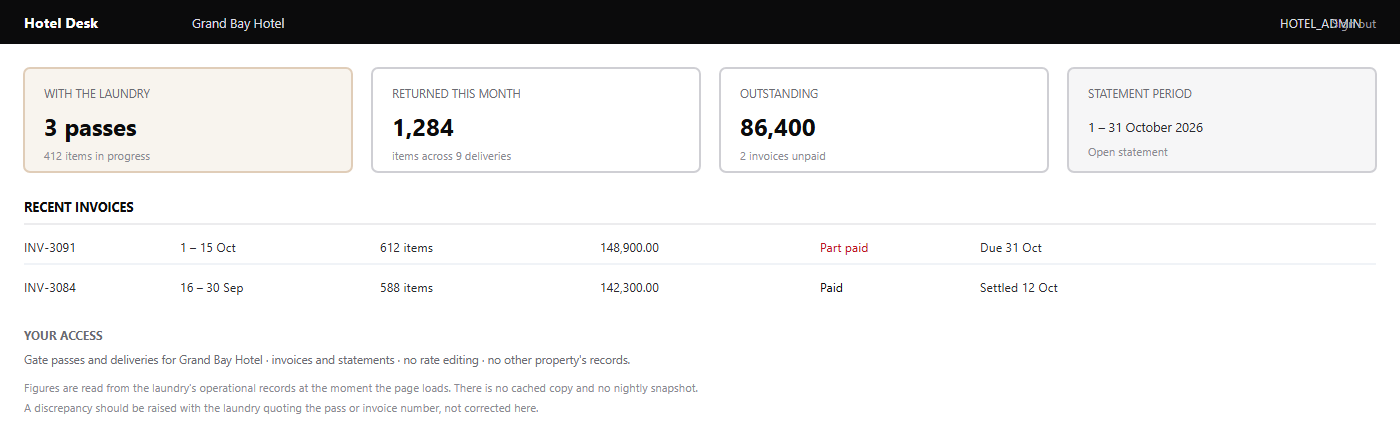
\includegraphics[width=\linewidth]{images/fig-16.png}
\caption{— Hotel Desk overview for a single property.Figure 16}
\end{figure}
\subsubsection*{Reading the tiles}
The four tiles are deliberately operational rather than analytical.  counts open gate passes and the items on them;  counts delivered items in the current calendar month;  is the unpaid balance across issued invoices; and the  links to the current statement. None of these figures includes another client's data, and none can be re-scoped by the hotel.\textbf{With the laundry}\textbf{returned this month}\textbf{outstanding}\textbf{statement period}

6 · User Manual — Hotel Desk AppLoveLaundry — System Manual

\begin{notebox}NoteA hotel cannot change the date range of a total on the overview. Period selection belongs to the statement, where the boundaries are explicit and the document is designed to be printed.\end{notebox}
\textsc{\small\color{crimson}6.3 · Gate passes}\par\medskip
\section*{Gate passes (hotel view)}
The hotel's gate-pass list shows every pass raised for its property: the date the goods were collected, the promised return date, the item count and the current status. It is the operational answer to “where is our linen?”

\begin{center}\small
\begin{tabularx}{\linewidth}{|X|X|}
\hline
\rowcolor{lightgrey}
\textbf{Column} & \textbf{Meaning} \\ \hline
Pass number & The laundry's reference; quote it in any query \\ \hline
Received & Date the laundry took possession of the goods \\ \hline
Due back & Promised return date \\ \hline
Items & Total quantity on the pass \\ \hline
Status & Received, in wash, ready, delivered, closed \\ \hline
Last update & When the status last changed \\ \hline
\end{tabularx}
\end{center}
\subsubsection*{What the hotel can see on a pass}
The hotel sees the items, the quantities, the service type and the status history. It does not see rates on the pass view — pricing is a commercial matter between the laundry and the property, stated on the invoice — and it never sees the laundry's internal cost, worker assignment or route information.

\subsubsection*{Procedure — finding a pass}
\begin{enumerate}
\item Open .\textbf{Gate passes}
\item Filter by date range if you know when the goods were collected, or search by pass number from the laundry's collection note.
\item Open the pass to see its item lines and status history.
\item If the status has not moved when you expect it to, contact the laundry quoting the pass number rather than raising a new pass; there is no way to create a pass from this application.
\end{enumerate}
\begin{notebox}WarningA hotel cannot create, edit or cancel a gate pass. A missing pass is a laundry-side data entry issue: report it with the collection date and the driver's name, and the laundry will raise or correct it.\end{notebox}
\textsc{\small\color{crimson}6.4 · Deliveries}\par\medskip
\section*{Deliveries (hotel view)}
Deliveries show what has come back, when, and in what quantity. For a hotel, this is the operational record that supports housekeeping's own counts — and the evidence used when an invoice quantity is questioned.

6 · User Manual — Hotel Desk AppLoveLaundry — System Manual

\begin{center}\small
\begin{tabularx}{\linewidth}{|X|X|}
\hline
\rowcolor{lightgrey}
\textbf{Field} & \textbf{Why it matters} \\ \hline
Delivery date and time & Matches the property's receiving log \\ \hline
Pass reference & Links the delivery to what was sent \\ \hline
Items and quantities & What was actually returned, line by line \\ \hline
Received by & The name recorded by the laundry at handover \\ \hline
Partial indicator & Shows that a pass is only partly returned \\ \hline
\end{tabularx}
\end{center}
\subsubsection*{Partial deliveries}
A pass may come back in several deliveries. The hotel sees each one separately, with the outstanding quantity on the pass. This is normal for large properties where sheets and towels are processed in different batches, and it is not a discrepancy.

\subsubsection*{Procedure — reconciling a delivery}
\begin{enumerate}
\item Open  and filter to the date of receipt.\textbf{Deliveries}
\item Compare the quantities on each delivery with the property's receiving sheet, line by line.
\item Where a line differs, note the pass number, the item and both quantities before contacting the laundry.
\item Report the difference the same day. A difference found a week later cannot be checked against the laundry floor.
\item Do not sign for a delivery you have not counted; the recorded receiver is the evidence that the count was accepted.
\end{enumerate}
\begin{notebox}NoteDeliveries are read-only here. If a count was signed for in error, the correction is made by the laundry and appears in the history, including the reason.\end{notebox}
\textsc{\small\color{crimson}6.5 · Invoices}\par\medskip
\section*{Invoices}
An invoice is the hotel's bill: quantities delivered in a period, at the agreed rates, with tax and the balance outstanding. The hotel can open an invoice, read its lines and download it — but it cannot alter it, and it cannot raise one.

\begin{center}\small
\begin{tabularx}{\linewidth}{|X|X|}
\hline
\rowcolor{lightgrey}
\textbf{State} & \textbf{What it means for the property} \\ \hline
Issued & Payable; the amount due is shown on the invoice \\ \hline
Part paid & Some payment has been recorded; the remainder is shown \\ \hline
Paid & Settled in full; no action required \\ \hline
Void & Cancelled by the laundry; a replacement may exist — check the statement \\ \hline
\end{tabularx}
\end{center}
6 · User Manual — Hotel Desk AppLoveLaundry — System Manual

\subsubsection*{Procedure — checking an invoice}
\begin{enumerate}
\item Open  and select the period or invoice number.\textbf{Invoices}
\item Open the invoice and compare its lines with your own receiving records for the same period.
\item Download the PDF if you need it for internal approval. The download is the same document the laundry holds.
\item Where a line is disputed, quote the invoice number, the line and the pass reference in your query to the laundry.
\item Do not withhold payment for one disputed line without telling the laundry: a short payment without explanation appears as an aged balance and may suspend service.
\end{enumerate}
\subsubsection*{What an invoice does not show}
Invoices state quantities and agreed rates. They do not show the laundry's internal costs, worker productivity, other clients' rates, or the composition of any discount beyond the line description. Those are outside the client relationship and are not exposed by any hotel endpoint.

\begin{notebox}WarningIf an invoice includes a pass you do not recognise, do not pay it and do not ignore it. Report it with the pass number the same day; a misposted pass is easy to correct before the period closes and hard afterwards.\end{notebox}
\textsc{\small\color{crimson}6.6 · Statements}\par\medskip
\section*{Statements}
A statement lists every invoice, payment and adjustment for a period with a running balance. It is the document a hotel's finance team reconciles against its own ledger, and it is the reason the portal exists for many properties.

\begin{center}\small
\begin{tabularx}{\linewidth}{|X|X|}
\hline
\rowcolor{lightgrey}
\textbf{Section} & \textbf{Content} \\ \hline
Opening balance & Amount outstanding at the start of the period \\ \hline
Invoices & Each invoice with date, number and amount \\ \hline
Payments & Each payment received, with method and reference \\ \hline
Adjustments & Credit notes and corrections, each with a reason \\ \hline
Closing balance & Opening balance plus invoices, less payments and credits \\ \hline
\end{tabularx}
\end{center}
\subsubsection*{Procedure — reconciling a statement}
6 · User Manual — Hotel Desk AppLoveLaundry — System Manual

\begin{enumerate}
\item Open  and select the period. The default is the current month to date.\textbf{Statements}
\item Print or download the statement for your finance file.
\item Match each invoice to your approved purchase record.
\item Match each payment to your bank or petty-cash record. A payment recorded by the laundry but not yet cleared in your bank will appear here before it appears there — that is timing, not error.
\item Query any unmatched line with its reference. The closing balance is the figure that must agree, not the individual lines alone.
\end{enumerate}
\begin{notebox}NoteStatements are generated on request from the laundry's records. A statement downloaded twice in a day may differ if a payment was posted in between, so always keep the version you reconciled against.\end{notebox}
\textsc{\small\color{crimson}6.7 · What a hotel can and cannot do}\par\medskip
\section*{What a hotel can and cannot do}
The hotel portal is read-only by design. The table below is the complete statement of a hotel account's authority; anything not listed as permitted is refused by the server, not merely hidden in the interface.

\begin{center}\small
\begin{tabularx}{\linewidth}{|X|X|X|}
\hline
\rowcolor{lightgrey}
\textbf{Action} & \textbf{Permitted} & \textbf{Notes} \\ \hline
View own gate passes & Yes & Filtered by laundry\_id and client\_name \\ \hline
View own deliveries & Yes & Includes partial deliveries \\ \hline
View and download own invoices & Yes & Issued documents only; drafts are invisible \\ \hline
View and download own statements & Yes & Any period within retention \\ \hline
Create or edit a gate pass & No & Laundry staff only \\ \hline
Record or amend a delivery & No & Laundry staff only \\ \hline
Raise, edit or void an invoice & No & Issued invoices are immutable for everyone \\ \hline
Post a payment & No & Payments are recorded by the laundry \\ \hline
View another property's records & No & Different client\_name; no endpoint accepts a name parameter \\ \hline
View rates, costs or worker data & No & Outside the client relationship \\ \hline
Manage hotel user accounts & No & HOTEL\_ADMIN manages its own users only through the laundry \\ \hline
\end{tabularx}
\end{center}
\subsubsection*{Why read-only}
A hotel that could edit its own records could dispute an invoice by changing the evidence. Making the portal read-only removes that possibility entirely and makes the portal's data credible to both parties: what the hotel sees is exactly what the laundry recorded, unmediated.

\begin{notebox}NoteHOTEL\_ADMIN and HOTEL\_MANAGER differ in what they can see of the account's commercial detail, not in what they can change. Neither role can change operational data.\end{notebox}
6 · User Manual — Hotel Desk AppLoveLaundry — System Manual

\textsc{\small\color{crimson}6.8 · Procedures}\par\medskip
\section*{Hotel desk procedures}
These are the five tasks a hotel performs in the portal. All of them end in reading or downloading; none of them changes a laundry record.

\subsubsection*{Procedure — checking what is still with the laundry}
\begin{enumerate}
\item Open  and read the  tile.\textbf{Overview}\emph{with the laundry}
\item Open  and filter to open statuses.\textbf{Gate passes}
\item For each pass, check the due-back date against housekeeping's requirement for the coming days.
\item If a pass is overdue, contact the laundry with the pass number and the date it was due.
\end{enumerate}
\subsubsection*{Procedure — preparing a month-end reconciliation}
\begin{enumerate}
\item Open  and select the closed month.\textbf{Statements}
\item Download the statement and every invoice referenced on it.
\item Match invoices to approved purchase records and payments to bank entries.
\item Record any unmatched item with its reference and raise a single consolidated query with the laundry.
\end{enumerate}
\subsubsection*{Procedure — reporting a discrepancy}
Collect the pass number or invoice number, the item description, the quantity you counted and the date. Send them in one message to the laundry's client contact. A query with references is resolved in minutes; a query without them requires the laundry to reconstruct the day.

\begin{notebox}WarningDo not open a second account to check another property, and do not share credentials between properties. Each client account is scoped to one property; sharing it is a breach of the terms of use and destroys the audit trail.\end{notebox}
\textsc{\small\color{crimson}6.9 · Common errors and support}\par\medskip
\section*{Hotel desk — common errors and support}
6 · User Manual — Hotel Desk AppLoveLaundry — System Manual

\begin{center}\small
\begin{tabularx}{\linewidth}{|X|X|X|}
\hline
\rowcolor{lightgrey}
\textbf{Message} & \textbf{Cause} & \textbf{Action} \\ \hline
401 — invalid credentials & Wrong password, or a staff account used on the client endpoint & Use the hotel client account; ask the laundry to reset if forgotten \\ \hline
403 — client scope not resolved & Account exists but is not linked to a laundry and client\_name & Ask the laundry to correct the client account \\ \hline
404 — not found & The record belongs to another property & Check the reference; do not retry with a different account \\ \hline
No invoices for this period & Invoices not yet issued for the period & Ask the laundry when the period will be billed \\ \hline
Session ended & 12-hour client token expired & Sign in again \\ \hline
Statement shows an unknown invoice & Pass posted to this property in error & Report the invoice and pass number the same day \\ \hline
\end{tabularx}
\end{center}
\subsubsection*{Support path}
The hotel's first contact is the laundry that issued the account: they own the records, the invoicing and the client account itself. The laundry escalates to the platform operator only for authentication faults that survive a password reset — for example, a client account whose scope is missing or a token that is refused by every endpoint.

\subsubsection*{What to include in a support request}
\begin{itemize}
\item The property name and the client account email (never the password).
\item The exact message text and the time it occurred.
\item The pass or invoice number involved.
\item What you expected to see and what you saw instead.
\end{itemize}
\begin{notebox}NoteHotel accounts are created and disabled by laundry administrators in the user-service client account screen. A hotel cannot create its own account, and there is no self-service registration.\end{notebox}
\textsc{\small\color{crimson}6.10 · Hotel portal request path}\par\medskip
\section*{Hotel portal request path}
How one property's records are separated from every other property's, on every request.

6 · User Manual — Hotel Desk AppLoveLaundry — System Manual

\begin{figure}[htbp]
\centering
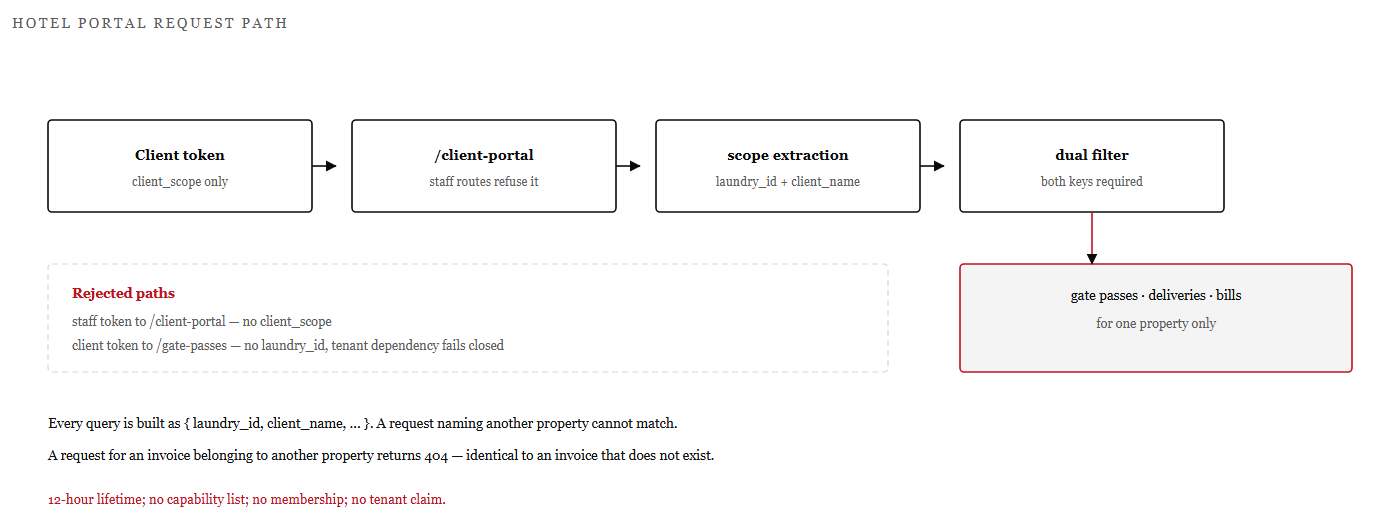
\includegraphics[width=\linewidth]{images/fig-17.png}
\caption{— Request path from a client token to a scoped query, with the rejected paths shown.Figure 17}
\end{figure}
The portal has no endpoint that accepts a client name as a parameter. The name comes from the token's scope, so a hotel cannot ask for another property's records even by guessing an identifier.

The dual filter is the mechanism: every query carries both the laundry and the client name. Filtering on the name alone would be unsafe across laundries; filtering on the laundry alone would expose every hotel to every other hotel.

\begin{notebox}RuleA request for another property's invoice returns not-found, identical to an invoice that does not exist. The portal never confirms that another property's records exist.\end{notebox}
\textsc{\small\color{crimson}Part Two · User Manual — Linen Room App}\par\medskip
\chapter{User Manual — Linen Room App}
\begin{quote}\itshape Scan-driven tracking of every tagged item, from collection to retirement.\end{quote}
\section{7.1 Overview and scanning}
The Linen Room app is the linen-room-app front end, used on a tablet or handheld at the wash station. Its users work one-handed with a scanner, so the interface is a single scan field, a large current-item card, and a short list of valid next actions. Everything else is history.

\begin{center}\small
\begin{tabularx}{\linewidth}{|X|X|}
\hline
\rowcolor{lightgrey}
\textbf{Attribute} & \textbf{Value} \\ \hline
Application & linen-room-app — React 19, TypeScript, Vite 8, Tailwind 4 \\ \hline
Development port & 5176 \\ \hline
Sign-in & Staff sign-in against user-service \\ \hline
Session key & ll\_linen\_session \\ \hline
Roles & LINEN\_SUPERVISOR, HOUSEKEEPER \\ \hline
Capabilities & linen:read, linen:scan, linen:write \\ \hline
\end{tabularx}
\end{center}
\subsection*{Why scanning, not typing}
7 · User Manual — Linen Room AppLoveLaundry — System Manual

A typed tag number is a guess with a keyboard. A scan is the identifier itself. The platform therefore treats the scan as the only way a lifecycle status advances: there is no “set status” dropdown, and no bulk action that moves items without reading them. If an item was not scanned, the record says it was not scanned — which is the truth the laundry needs when a client disputes a count.

\subsubsection*{Procedure — starting a shift at the station}
\begin{enumerate}
\item Sign in on the station device with your own linen-room account.
\item Confirm the station name and the current batch or pass shown at the top.
\item Test the scanner by scanning any tag already in hand; the item card should populate within a moment.
\item Keep the scan field focused. If a scan produces no response, tap the field before scanning again rather than retyping the tag.
\end{enumerate}
\begin{notebox}WarningDo not share a station login between staff. Every scan is attributed to the signed-in user, and an unattributable scan is worthless when a discrepancy is investigated.\end{notebox}
\textsc{\small\color{crimson}7.2 · Lifecycle statuses}\par\medskip
\section*{Lifecycle statuses}
Each tag moves through a fixed sequence. Statuses advance only by recording the action that caused the move, and each action is attributed to a user and a time. The sequence is enforced server-side: a scan that would skip a stage is rejected.

\begin{figure}[htbp]
\centering
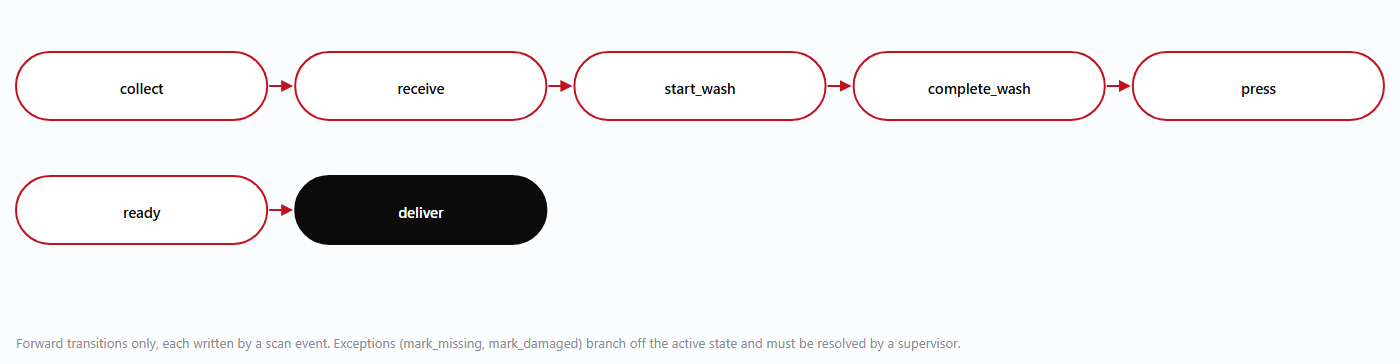
\includegraphics[width=\linewidth]{images/fig-18.png}
\caption{— Linen state machine. Exceptions (, , ) branch from the active state.Figure 18mark\_missingmark\_damagedretire}
\end{figure}
7 · User Manual — Linen Room AppLoveLaundry — System Manual

\begin{center}\small
\begin{tabularx}{\linewidth}{|X|X|X|}
\hline
\rowcolor{lightgrey}
\textbf{Action} & \textbf{From → to} & \textbf{When it is used} \\ \hline
collect & new → collected & Goods picked up from the client or from the property's linen room \\ \hline
receive & collected → received & Counted in at the laundry; discrepancies are raised here \\ \hline
start\_wash & received → in wash & Loaded into a wash batch \\ \hline
complete\_wash & in wash → washed & Batch finished; items awaiting finishing \\ \hline
press & washed → pressed & Ironed or folded and inspected \\ \hline
ready & pressed → ready & Racked and available for delivery \\ \hline
deliver & ready → delivered & Handed to the client against a delivery \\ \hline
mark\_missing & any active → missing & Item cannot be found; requires a supervisor \\ \hline
mark\_damaged & any active → damaged & Item is damaged; requires a supervisor \\ \hline
retire & any → retired & Item withdrawn from service permanently \\ \hline
\end{tabularx}
\end{center}
\begin{notebox}NoteThere is no reverse transition. An item scanned into the wrong batch is corrected by recording the exception and re-scanning it into the correct batch, which leaves both events visible.\end{notebox}
\textsc{\small\color{crimson}7.3 · Scan workflow}\par\medskip
\section*{Scan workflow}
The station screen is built around one loop: scan, confirm, act. The current item card shows what the platform knows, and the action buttons show only what is legal next — which is how a fast operator avoids invalid transitions without memorising the rules.

\begin{figure}[htbp]
\centering
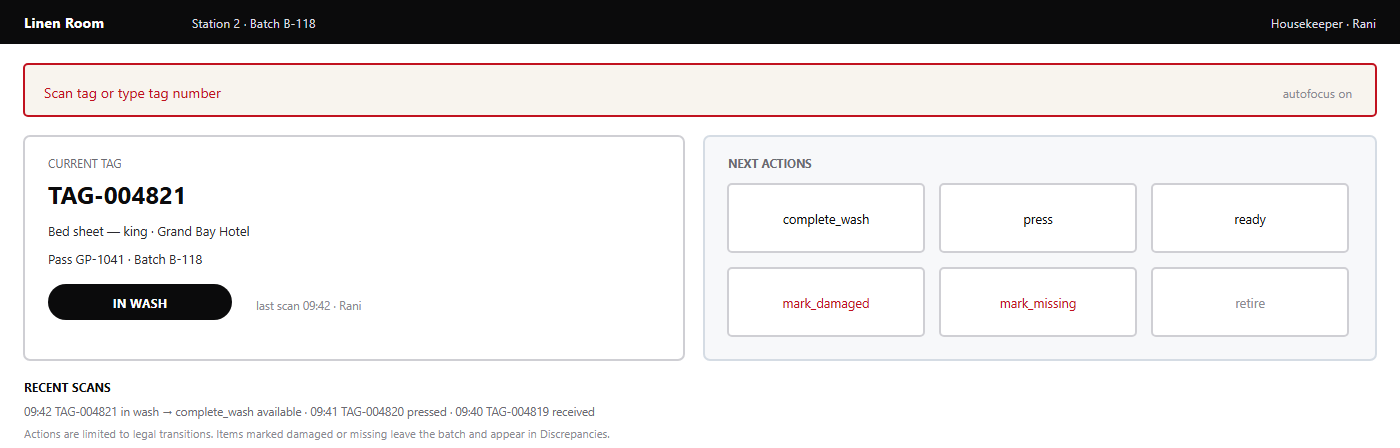
\includegraphics[width=\linewidth]{images/fig-19.png}
\caption{— Scan station: scan field, current tag card and legal next actions.Figure 19}
\end{figure}
\subsubsection*{Procedure — scanning a batch through}
7 · User Manual — Linen Room AppLoveLaundry — System Manual

\begin{enumerate}
\item Scan the tag. The current tag card confirms the item and its current status.
\item Check the item against the card — type, client and pass. A scan of the wrong item is worse than no scan.
\item Select the next action. Only legal transitions are offered. The list updates immediately.
\item Repeat for each item. The batch counter increments as items advance.
\item When the batch is complete, confirm the batch total on screen against the physical count before moving the load.
\end{enumerate}
\begin{notebox}NoteScanning is idempotent: scanning the same tag twice for the same action does not duplicate the event. It is safer to scan again than to assume a scan registered.\end{notebox}
\textsc{\small\color{crimson}7.4 · Inventory}\par\medskip
\section*{Inventory}
Inventory is the count of tags by status, item type and client. It is derived from scan history, so it is a live picture rather than a periodic stock take — and it is only as accurate as the scanning discipline behind it.

\begin{center}\small
\begin{tabularx}{\linewidth}{|X|X|X|}
\hline
\rowcolor{lightgrey}
\textbf{View} & \textbf{Shows} & \textbf{Use} \\ \hline
By status & Tags in each lifecycle state & See what is in wash, ready or missing at a glance \\ \hline
By item type & Sheets, duvet covers, towels, mats and so on & Capacity planning and reorder decisions \\ \hline
By client & Tags attributable to each client\_name & Client-level reconciliation and loss conversations \\ \hline
By age & Tags whose current status is older than expected & Find items stuck in a stage \\ \hline
Retired & Tags withdrawn from service & Asset history and replacement rate \\ \hline
\end{tabularx}
\end{center}
\subsubsection*{What inventory is not}
It is not a valuation. The platform counts tags and items, not their book value; asset accounting belongs to the accounting service and to the laundry's own fixed-asset register. It is also not a guarantee of physical presence: a tag can be scanned and then lost, which is exactly what the discrepancy process exists to catch.

\subsubsection*{Procedure — daily inventory check}
\begin{enumerate}
\item Open  and select .\textbf{Inventory}\textbf{By status}
\item Compare the  count with the batches physically on the floor. A large difference means items were loaded without scanning.\emph{in wash}
\item Compare  with the rack. Ready items that are not on the rack are either delivered without a scan or missing.\emph{ready}
\item Check  for items in one status for longer than the wash cycle allows.\textbf{By age}
\item Record any unexplained difference through the discrepancy process rather than adjusting the count.
\end{enumerate}
7 · User Manual — Linen Room AppLoveLaundry — System Manual

\begin{notebox}WarningNever correct inventory by retiring items to make the numbers match. Retirement is permanent and removes the asset from service; a missing item may still be found.\end{notebox}
\textsc{\small\color{crimson}7.5 · Discrepancies}\par\medskip
\section*{Discrepancies}
A discrepancy is a recorded mismatch: an item counted in short, found damaged, or unaccounted for at the end of a batch. The platform records discrepancies rather than smoothing them away, because a pattern of loss is only visible if each instance survives.

\begin{center}\small
\begin{tabularx}{\linewidth}{|X|X|X|}
\hline
\rowcolor{lightgrey}
\textbf{Type} & \textbf{Raised when} & \textbf{Effect} \\ \hline
Short receipt & Fewer items received than the pass states & Pass line quantity is queried; client is notified \\ \hline
Missing & Item cannot be found after a search & Tag leaves the active batch; supervisor review \\ \hline
Damaged & Item is torn, stained beyond recovery or otherwise unusable & Tag marked damaged; client liability assessed \\ \hline
Short delivery & Fewer items delivered than the client expected & Pass remains open or is closed short with a reason \\ \hline
Unscanned & Item found physically but absent from the batch record & Item is scanned into the correct stage; cause noted \\ \hline
\end{tabularx}
\end{center}
\subsubsection*{Procedure — recording a missing item}
\begin{enumerate}
\item Search the station, the batch and the rack before recording anything. Most missing items are in the previous batch.
\item Scan or enter the tag and select .\textbf{mark\_missing}
\item Enter where it was last seen and what search was carried out.
\item Confirm. The item leaves the active batch and appears in open discrepancies.
\item Notify the supervisor, who decides whether to inform the client and whether to replace the item.
\end{enumerate}
\subsubsection*{Closing a discrepancy}
A discrepancy is closed when the item is found, when the client accepts the loss, or when it is written off with a reason. Closing is a supervisor action with an audit entry. An item found later is scanned back into the correct stage, which closes the missing record automatically and leaves both events in the tag's history.

\begin{notebox}NoteDiscrepancy counts are part of the dashboard for a reason: a laundry that never records a discrepancy is usually not counting, not not losing.\end{notebox}
\textsc{\small\color{crimson}7.6 · Tag printing}\par\medskip
\section*{Tag printing}
Tags are the physical identity of an item. Printing is therefore a controlled action: each printed tag is recorded, and a tag that is printed but never attached is a future discrepancy.

7 · User Manual — Linen Room AppLoveLaundry — System Manual

\begin{center}\small
\begin{tabularx}{\linewidth}{|X|X|}
\hline
\rowcolor{lightgrey}
\textbf{Rule} & \textbf{Reason} \\ \hline
Tags are printed in batches linked to an item type & Keeps numbering readable and simplifies replacement \\ \hline
A printed tag is recorded as issued & Allows an unattached tag to be traced \\ \hline
Duplicate tags are never printed for an active item & Two tags on one item double-counts inventory \\ \hline
A replacement tag is issued only after the old tag is retired & Prevents two live identities for one item \\ \hline
Printing requires linen:write & HOUSEKEEPER can scan but not print \\ \hline
\end{tabularx}
\end{center}
\subsubsection*{Procedure — printing a tag batch}
\begin{enumerate}
\item Open .\textbf{Tags → Print batch}
\item Choose the item type and the number of tags required.
\item Select the printer and confirm that labels are loaded — a half-printed batch wastes tag numbers.
\item Print, then apply each tag to an item immediately. Do not leave printed tags loose at the station.
\item Confirm the batch in the app so that the tags are recorded as issued and attached.
\end{enumerate}
\subsubsection*{Replacing a damaged tag}
Where a tag is unreadable but the item is identifiable, retire the old tag and issue a replacement, recording the reason. Where the item is not identifiable, treat it as an unscanned item: count it, assign it to the client whose linen it matches, and record how the identification was made. Guessing the client is worse than leaving the item unassigned.

\begin{notebox}WarningNever reprint an existing tag number onto a new label while the original is still attached. The item will be counted twice and the duplicate will be found months later during a reconciliation nobody can explain.\end{notebox}
\textsc{\small\color{crimson}7.7 · Procedures}\par\medskip
\section*{Linen room procedures}
The four procedures below cover a normal shift: receiving a pass, running a batch, delivering, and handing over at the end of the shift.

\subsubsection*{Procedure — receiving a pass}
\begin{enumerate}
\item Open the pass from the station's pass list.
\item Count the items physically, by type, before scanning anything.
\item Scan each tag as it is counted. Items without a tag are tagged first, then scanned.
\item Compare the scanned count with the pass quantity. Where it differs, record a short receipt with the count you found.
\item Confirm receipt. The pass moves to received and the items become available for batching.
\end{enumerate}
7 · User Manual — Linen Room AppLoveLaundry — System Manual

\subsubsection*{Procedure — running a wash batch}
\begin{enumerate}
\item Create a batch for the machine and load it.
\item Scan each item into the batch and select .\textbf{start\_wash}
\item At the end of the cycle, select  for the batch and scan out any item removed for separate treatment.\textbf{complete\_wash}
\item After pressing, scan each item and select , then  when it is racked.\textbf{press}\textbf{ready}
\end{enumerate}
\subsubsection*{Procedure — delivering from the linen room}
Delivery is recorded in the laundry app against the gate pass, not in the linen room. The linen room's part is to ensure that every item on the rack has been scanned to , so that the delivery quantity is supported by tag history. Where the linen room is also the dispatch point, scan the items out as  at handover so that the tag and the delivery agree.\emph{ready}\textbf{deliver}

\begin{notebox}NoteShift handover: confirm the batch count on screen matches the physical count, note any open discrepancies, and sign out. An unsigned station is an unattributable one.\end{notebox}
\textsc{\small\color{crimson}7.8 · Troubleshooting}\par\medskip
\section*{Linen room — troubleshooting}
\begin{center}\small
\begin{tabularx}{\linewidth}{|X|X|X|}
\hline
\rowcolor{lightgrey}
\textbf{Symptom} & \textbf{Likely cause} & \textbf{Action} \\ \hline
Scan produces nothing & Field lost focus, or scanner in keyboard-wedge mode disconnected & Tap the scan field and scan again; check the scanner cable or pairing \\ \hline
“Invalid transition” & Item is not in the state the action requires & Read the current status on the card; choose a legal action \\ \hline
“Tag not found” & Tag belongs to another laundry, or was never issued & Check the tag number against the print batch; do not create a duplicate \\ \hline
Item scanned twice & Double trigger or repeated scan & No action — scans are idempotent for the same action \\ \hline
Batch count does not match the rack & Item removed without scanning out & Scan the item to its actual stage; record an unscanned-item note \\ \hline
Cannot print tags & Role lacks linen:write & Ask a supervisor to print, or to adjust the role \\ \hline
\end{tabularx}
\end{center}
\subsubsection*{When the network is down}
The station cannot record scans without a connection to bill\_service. Do not continue scanning into a local file or a paper list and enter it later as if it happened in sequence: the timestamps would be false and the batch history misleading. Record the physical count on paper, keep the items segregated, and enter the scans when the connection returns, noting the delay. Chapter 11.4 describes what remains usable while a service is unavailable.

7 · User Manual — Linen Room AppLoveLaundry — System Manual

\subsubsection*{Escalation}
Escalate to a supervisor when an item cannot be identified, when a discrepancy involves more than a few items, or when a tag appears to exist in two batches. Escalate to the platform operator only when the application itself fails — a blank screen, a repeated server error, or a sign-in that fails for every user.

\begin{notebox}NoteReport the tag number and the exact message. A screenshot of the station screen is the fastest possible evidence.\end{notebox}
\textsc{\small\color{crimson}7.9 · Linen lifecycle state machine}\par\medskip
\section*{Linen lifecycle state machine}
Seven forward states, three exception states, and no way back.

\begin{figure}[htbp]
\centering
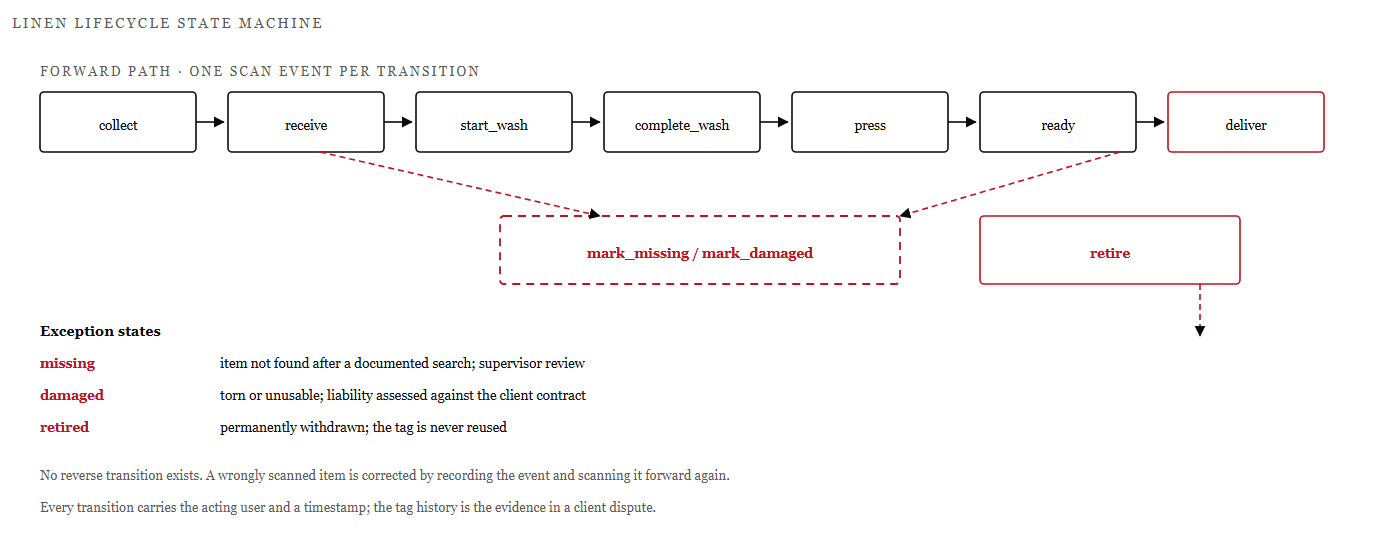
\includegraphics[width=\linewidth]{images/fig-20.png}
\caption{— The linen state machine with its exception branches. Transitions are written by scan events only.Figure 20}
\end{figure}
The scan procedure that writes these transitions is on page 75. The forward path is linear because the physical process is linear: goods are collected, received, washed, finished, pressed, made ready and delivered. Modelling it as a chain rather than a set of flags means an item cannot be simultaneously ready and in wash.

The exception states branch off the active state rather than replacing the chain. An item marked missing leaves the batch but keeps its history, so when it is found it can be scanned back into the correct stage without inventing a new tag.

\begin{notebox}RuleThere is no reverse transition and no status dropdown. A wrongly scanned item is corrected by recording the event and scanning it forward again, which leaves both facts visible.\end{notebox}
\part{Operating the Business}
\textsc{\small\color{crimson}Part Three · Administration and Configuration}\par\medskip
\chapter{Administration and Configuration}
\begin{quote}\itshape Creating tenants, granting access, and configuring an installation that can be rebuilt from documentation.\end{quote}
\section{8.1 Creating laundries}
A laundry is a tenant. Creating one is a platform operation performed by a , because it establishes the boundary inside which every later record will live. Laundry administrators cannot create tenants; they administer the one they belong to.\texttt{PLATFORM\_ADMIN}

\begin{center}\small
\begin{tabularx}{\linewidth}{|X|X|}
\hline
\rowcolor{lightgrey}
\textbf{Element} & \textbf{Purpose} \\ \hline
Name and short code & Display name and a stable short reference used on documents \\ \hline
Status & Active or suspended; a suspended tenant can sign in to read but not to write \\ \hline
Currency and tax configuration & Applied to every bill raised in the tenant \\ \hline
First administrator & An existing user granted ADMIN membership, or a new user created for the purpose \\ \hline
\end{tabularx}
\end{center}
\subsubsection*{Procedure — creating a laundry}
8 · Administration and ConfigurationLoveLaundry — System Manual

\begin{enumerate}
\item Sign in as a platform administrator and open the tenant administration screen.
\item Create the laundry: name, short code, currency and tax rate. Check the tax rate against the jurisdiction before saving — changing it later does not alter issued bills.
\item Create or select the first administrator's user account.
\item Add a membership linking that user to the new laundry with the ADMIN role.
\item Sign in as that administrator in a private window and confirm that the tenant name appears and that an empty dashboard loads.
\item Record the creation in the platform change log with the operator and the time.
\end{enumerate}
\begin{notebox}WarningDo not reuse a short code, even for a closed laundry. Short codes appear on printed documents and in exports; a reused code makes two businesses' history indistinguishable.\end{notebox}
\textsc{\small\color{crimson}8.2 · Users and memberships}\par\medskip
\section*{Users and memberships}
The platform separates a person from their access. A  is an identity — an email, a password hash, a display name. A  is that identity's link to one laundry, carrying a role. One person may hold memberships in several laundries and one role in each.\textbf{user}\textbf{membership}

\begin{center}\small
\begin{tabularx}{\linewidth}{|X|X|X|}
\hline
\rowcolor{lightgrey}
\textbf{Role} & \textbf{Give it to} & \textbf{Do not give it to} \\ \hline
ADMIN & The owner and at most one deputy & Every manager, by default \\ \hline
MANAGER & Supervisors who close days and handle money & Counter assistants \\ \hline
STAFF & Operational data entry & Anyone who approves refunds \\ \hline
LINEN\_SUPERVISOR & The person accountable for linen loss & Seasonal staff without handover responsibility \\ \hline
HOUSEKEEPER & Scanning and finishing staff & Anyone who prints tags or retires items \\ \hline
\end{tabularx}
\end{center}
\subsubsection*{Procedure — adding a user to a laundry}
\begin{enumerate}
\item Open  and select .\textbf{Users}\textbf{Add user}
\item Enter the person's own email address. Shared mailboxes and role-based addresses make the audit trail useless.
\item Set an initial password and require a change at first sign-in.
\item Add the membership: choose the laundry (fixed to your own tenant if you are not a platform administrator) and the role.
\item Ask the user to sign in while you are present, so that a mistyped address is discovered immediately.
\end{enumerate}
\subsubsection*{Removing access}
8 · Administration and ConfigurationLoveLaundry — System Manual

Removing someone's access means removing the membership or disabling the user, never deleting history. A deleted user leaves records attributed to nobody, which is exactly the situation an audit cannot tolerate. Disabling the user prevents new sign-ins; existing tokens remain valid until they expire, so a departure that requires immediate certainty also requires a signing-key rotation or a documented acceptance of the residual window.

\begin{notebox}NoteChanging a role takes effect at the next sign-in, because capabilities are carried in the token. If a change must apply immediately, disable the user and re-enable them so that a fresh token is issued.\end{notebox}
\textsc{\small\color{crimson}8.3 · Hotel client accounts and roles}\par\medskip
\section*{Hotel client accounts and roles}
Hotel accounts live in a separate collection from staff users, and they are created by the laundry that serves the hotel. The account binds an email and password to exactly one  within the laundry, which is the whole of its authority.\texttt{client\_name}

\begin{center}\small
\begin{tabularx}{\linewidth}{|X|X|}
\hline
\rowcolor{lightgrey}
\textbf{Field} & \textbf{Meaning} \\ \hline
Email & Sign-in identity for the hotel user \\ \hline
Password hash & Salted hash; never displayed or exported \\ \hline
laundry\_id & The tenant whose records the account may read \\ \hline
client\_name & The one hotel whose records are visible \\ \hline
Role & HOTEL\_ADMIN or HOTEL\_MANAGER \\ \hline
Status & Active or disabled \\ \hline
\end{tabularx}
\end{center}
\subsubsection*{Procedure — creating a hotel account}
\begin{enumerate}
\item Confirm the exact  spelling used on the hotel's gate passes and bills. A variant spelling creates an account that sees nothing.\texttt{client\_name}
\item Create the client account with the hotel's contact email and a role.
\item Communicate the credentials through a channel the hotel controls; never send a password in the same message as the sign-in address.
\item Ask the hotel to sign in and confirm they can see their own passes and invoices.
\item Record the creation and the operator in the change log.
\end{enumerate}
\subsubsection*{Enabling and disabling accounts}
A client account is disabled when a property changes management, when a member of staff leaves, or when credentials are suspected compromised. Disabling is immediate for new sign-ins and is recorded with the operator and reason. The endpoints are  for the account's own state,  for listing and creating accounts, and  for changing an account's state.\texttt{GET /client/auth/status}\texttt{GET|POST /clients}\texttt{PATCH /clients/\{id\}/status}

8 · Administration and ConfigurationLoveLaundry — System Manual

\begin{notebox}WarningNever create a client account with a staff role, and never add a client account to a membership. The two identity systems are separate so that a hotel token can never satisfy a staff authorisation check.\end{notebox}
\textsc{\small\color{crimson}8.4 · Environment variables}\par\medskip
\section*{Environment variables}
Configuration is supplied through the environment. Nothing that differs between installations is compiled into the code, and nothing secret is committed to the repository. The table lists the variables an operator must set; names follow the service that reads them.

\begin{center}\small
\begin{tabularx}{\linewidth}{|X|X|X|}
\hline
\rowcolor{lightgrey}
\textbf{Variable} & \textbf{Read by} & \textbf{Purpose} \\ \hline
MONGO\_URI & All services & Database connection string, with TLS and the service's own credential \\ \hline
DB\_NAME & Per service & The database the service owns (user\_db, operations, accounting) \\ \hline
JWT\_SIGNING\_KEY & user-service & Signs staff tokens; rotated on the schedule in 13.4 \\ \hline
JWT\_VERIFY\_KEYS & All services & Key set used to verify tokens, including the next key during rotation \\ \hline
JWT\_TTL\_STAFF / JWT\_TTL\_CLIENT & user-service & Token lifetimes: 24 hours and 12 hours \\ \hline
KEK\_ID / KEK\_MATERIAL & bill\_service, user-service & Key-encryption key reference and material for envelope encryption \\ \hline
SEARCH\_KEY & bill\_service & HMAC key for deterministic search tokens \\ \hline
CORS\_ORIGINS & All services & Exact front-end origins permitted to call the API \\ \hline
LOG\_LEVEL & All services & Verbosity; production defaults to structured informational logging \\ \hline
RATE\_LIMIT\_* & Proxy and services & Thresholds per class, as described in 3.5 \\ \hline
\end{tabularx}
\end{center}
\subsubsection*{Front-end configuration}
Each React application reads build-time variables prefixed . Only public values belong there — service base URLs, environment name, feature flags — because everything so prefixed is embedded in the bundle and readable by anyone with a browser. A secret placed in a  variable is published, not configured.\texttt{VITE\_}\texttt{VITE\_}

\begin{verbatim}
VITE_API_BASE=/api
VITE_ENV=production
VITE_ENABLE_AI_ASSIST=true
\end{verbatim}
\begin{notebox}WarningChanging a signing key or a KEK is not a routine configuration edit. Follow the rotation procedures in 3.6; an unplanned change invalidates every session or makes encrypted fields unreadable.\end{notebox}
\textsc{\small\color{crimson}8.5 · Deployment steps}\par\medskip
\section*{Deployment steps}
A deployment is a build, a configuration check, a service restart and a smoke test — in that order. The steps below assume a single application host behind a reverse proxy, as described in 2.9.

8 · Administration and ConfigurationLoveLaundry — System Manual

\subsubsection*{Procedure — deploying a release}
\begin{enumerate}
\item Build the four front-end bundles from the tagged commit. Record the commit hash in the change log.
\item Confirm the environment file contains every required variable, and that no secret is present in a  variable.\texttt{VITE\_}
\item Apply any database index changes for the release. Index creation is online in MongoDB and must precede the code that depends on it.
\item Stop and restart each service in dependency order: user-service, bill\_service, then the supporting services.
\item Verify health: sign in as a staff user, load the dashboard, open a gate pass, and confirm the hotel portal rejects a staff token.
\item Publish the new static bundles. Because filenames are hashed, the old bundles remain valid until the proxy switch.
\item Watch the error log for five minutes, then declare the release complete — or roll back by restoring the previous bundle and the previous service version.
\end{enumerate}
\begin{center}\small
\begin{tabularx}{\linewidth}{|X|X|X|}
\hline
\rowcolor{lightgrey}
\textbf{Symptom} & \textbf{Rollback?} & \textbf{Note} \\ \hline
Sign-in failing for everyone & Yes, immediately & Usually a key or configuration mismatch \\ \hline
One screen erroring & No & Fix forward; rollback does not restore data written since \\ \hline
Bills wrong after release & Yes, and stop writes & Preserve the database state before any further action \\ \hline
Slow but functional & No & Investigate before rolling back a working system \\ \hline
\end{tabularx}
\end{center}
\begin{notebox}WarningNever deploy on a Friday afternoon or immediately before a day close. A release that fails at close leaves the business unable to bill, and the person who can fix it is least available.\end{notebox}
\textsc{\small\color{crimson}Part Three · Disaster Management}\par\medskip
\chapter{Disaster Management}
\begin{quote}\itshape What can go wrong, how bad it would be, and who does what in the first hour.\end{quote}
\section{9.1 Framework and risk method}
Disaster management here means the decisions made before an incident, so that during one nobody has to invent a process. The framework has four parts: a risk register that names and ranks the threats, a severity matrix that determines the response, a runbook that sequences the first hour, and a review that turns each incident into a change.

Risks are scored on likelihood and impact, each on a three-point scale. Likelihood reflects the platform's actual exposure — a single application host, one replica set, a small team — not a hypothetical adversary. Impact reflects the business consequence: whether the laundry can trade, whether records are lost, and whether obligations to clients are breached.

\begin{center}\small
\begin{tabularx}{\linewidth}{|X|X|X|}
\hline
\rowcolor{lightgrey}
\textbf{Score} & \textbf{Likelihood} & \textbf{Impact} \\ \hline
High & Expected within a year on current controls & Trading stops, or data is lost or exposed \\ \hline
Medium & Possible within one to three years & A function is unavailable for hours, or figures are unreliable \\ \hline
Low & Unlikely without a change in circumstances & Local inconvenience, recoverable within a shift \\ \hline
\end{tabularx}
\end{center}
\section{9.2 Risk register}
9 · Disaster ManagementLoveLaundry — System Manual

The register is reviewed quarterly and after every Severity 1 or 2 incident. Likelihood and impact are re-scored then; an entry that has not changed for a year is either genuinely stable or not being examined.

\begin{center}\small
\begin{tabularx}{\linewidth}{|X|X|X|X|X|}
\hline
\rowcolor{lightgrey}
\textbf{Risk} & \textbf{Likelihood} & \textbf{Impact} & \textbf{Mitigation} & \textbf{Owner} \\ \hline
Database corruption or loss & Low & High & Nightly logical backups, oplog retention, quarterly restore drills & Platform operator \\ \hline
Staff credential compromise & Medium & High & Short token lifetime, capability checks, sign-in auditing, rapid disable and key rotation & Laundry administrator \\ \hline
Ransomware on the application host & Low & High & Immutable off-host backups, least-privilege accounts, no interactive browsing on the host & Platform operator \\ \hline
Insider misuse of discounts or voids & Medium & Medium & Reason codes, supervisor approval, reprint detection, day-close reconciliation & Laundry owner \\ \hline
Cloud region outage & Low & High & Documented rebuild in a second region, configuration held outside the region, DNS switch & Platform operator \\ \hline
Payment or messaging supplier outage & Medium & Medium & Manual fallback recorded in the day book, reconciliation on recovery & Laundry manager \\ \hline
Disk exhaustion on the database host & Medium & High & Capacity alerts, log rotation, backup pruning, retention policy & Platform operator \\ \hline
Key loss (KEK or signing key) & Low & High & Escrowed KEK, documented rotation, staged key overlap & Platform operator \\ \hline
Silent billing error after a release & Medium & High & Suite gates, no Friday deploys, day-close review of unbilled items & Developer \\ \hline
\end{tabularx}
\end{center}
\begin{notebox}NoteThe last entry is the one most often missed. A release that produces subtly wrong bills is worse than an outage, because nobody notices until clients do.\end{notebox}
\textsc{\small\color{crimson}9.3 · Threat scenarios}\par\medskip
\section*{Threat scenario — database loss}
The operations database is lost or corrupted: a failed migration, an accidental drop, or storage failure on the primary. Sign-in still works, because user\_db is intact, which makes the incident look smaller than it is — staff can reach a dashboard that shows nothing.\textbf{Scenario.}

\subsubsection*{Immediate signs}
\begin{itemize}
\item Every list view returns empty or errors while sign-in succeeds.
\item Service logs show connection failures or authentication errors against the operations database.
\item The MongoDB primary is unavailable and no election completes.
\end{itemize}
\subsubsection*{First actions}
9 · Disaster ManagementLoveLaundry — System Manual

\begin{enumerate}
\item Stop writes. Take bill\_service out of the proxy rotation so that no partial records are created against a broken store.
\item Confirm the scope: is the database unreachable, corrupted, or empty? These have different recovery paths.
\item Check the replica set state and the most recent successful backup timestamp before attempting any repair.
\item Declare severity: database loss affecting trading is Severity 1, and the response clock starts now.
\item Begin the restore procedure in 10.4 in the fixed order: user\_db, operations, accounting.
\item Notify the laundry's manager with a factual statement and an expected next update time, not an estimate of recovery.
\end{enumerate}
\subsubsection*{What not to do}
Do not run a repair against the only copy. Do not restore over a database that might still be recoverable in place. Do not restart every service at once — the restart destroys the evidence in memory and makes the timeline harder to reconstruct. And do not accept a restored database without the verification steps in 10.5; a restore that loses yesterday's bills is a second incident.

\begin{notebox}WarningIf the loss is caused by a delete or a bad migration, point-in-time recovery (10.6) is almost always better than restoring last night's backup. Restore the backup only when the oplog cannot cover the window.\end{notebox}
\textsc{\small\color{crimson}9.3 · Threat scenarios (continued)}\par\medskip
\section*{Threat scenario — credential compromise}
A staff password is phished, or a token is copied from a shared terminal. Because tokens are stateless, the attacker can act as that user until the token expires — up to 24 hours — and every action will be attributed to the real person.\textbf{Scenario.}

\subsubsection*{Detection}
\begin{itemize}
\item Sign-ins from unfamiliar addresses or at unusual hours, visible in the authentication log.
\item A burst of record creation or payment posting by one account.
\item A user reporting that they were signed out unexpectedly, or that records exist they did not create.
\end{itemize}
\subsubsection*{Containment}
9 · Disaster ManagementLoveLaundry — System Manual

\begin{enumerate}
\item Disable the affected user immediately. This prevents new tokens even though it does not revoke the existing one.
\item Identify the capability of the compromised account: a STAFF token can create passes; an ADMIN token can change users.
\item If the account held ADMIN or the token may have reached a privileged surface, rotate the signing key to invalidate every session (3.6).
\item Preserve logs and audit entries before rotating, so the attacker's actions remain reconstructible.
\item Review the account's actions during the exposure window and reverse anything fraudulent through the normal correction paths — never by editing records directly.
\item Notify affected clients if their data was accessed, following 9.6.
\end{enumerate}
\subsubsection*{Afterwards}
Force a password reset for the user, review whether the password was reused elsewhere, and check whether the compromise came from a shared terminal. The most common root cause is not a sophisticated attack but a password written beside a counter terminal, and the control that fixes it is a lock screen and individual accounts.

\begin{notebox}WarningDo not simply change the user's password. The existing token remains valid until expiry; disabling the account or rotating the key is the only way to stop it.\end{notebox}
\textsc{\small\color{crimson}9.3 · Threat scenarios (continued)}\par\medskip
\section*{Threat scenario — ransomware and insider misuse}
\subsection*{Ransomware on the application host}
The host is encrypted by ransomware, either through a compromised remote-access account or through a downloaded file. The application stops; the database may be on the same host or reachable from it.\textbf{Scenario.}

\begin{enumerate}
\item Isolate the host from the network immediately. Do not shut it down if evidence may be needed, but do isolate it.
\item Confirm that off-host backups exist and are immutable. This is the moment the design decision in 10.1 proves itself.
\item Do not pay, and do not attempt decryption on the production host.
\item Build a clean host from the documented deployment steps (8.5), then restore data (10.4).
\item Rotate every credential the host could read: database users, storage keys, signing keys, KEK if it was present on the host.
\item Report the incident, including any personal data exposure, per 9.6.
\end{enumerate}
\subsection*{Insider misuse}
A member of staff issues refunds to themselves, voids bills after taking cash, applies discounts for friends, or exports client data. The pattern is usually small and repeated rather than large and obvious.\textbf{Scenario.}

9 · Disaster ManagementLoveLaundry — System Manual

\begin{itemize}
\item reason codes, supervisor approval for refunds and discounts, capability separation between counter staff and managers, and no shared logins.\textbf{Prevention:}
\item review refund and void frequency per user, compare discounts against the standard, and reconcile the drawer daily rather than monthly.\textbf{Detection:}
\item preserve the audit records, involve the owner before confronting anyone, and correct the financial records through adjustment documents so that the client's statement stays true.\textbf{Response:}
\end{itemize}
\begin{notebox}NoteAudit records are append-only and are the reason insider misuse is provable at all. Any proposal to allow editing or deleting audit entries should be refused on these grounds alone.\end{notebox}
\textsc{\small\color{crimson}9.3 · Threat scenarios (continued)}\par\medskip
\section*{Threat scenario — region outage and supplier outage}
\subsection*{Cloud region outage}
The region hosting the application and database becomes unavailable: a provider incident, a network partition, or a sustained control-plane failure. Both the application and its primary database are unreachable, and the provider's own console may be degraded too.\textbf{Scenario.}

\begin{enumerate}
\item Confirm the outage is the provider's, not yours: check status pages from outside the region and test connectivity from a second location.
\item Declare Severity 2 (or 1 if trading is impossible during business hours) and start the communication plan in 9.7.
\item Do not attempt to rebuild in a second region until the provider confirms the primary region's state; a split-brain restore is worse than an outage.
\item When confirmed unrecoverable within the business window, provision the second region from the documented steps, restore the latest off-host backup, and repoint DNS.
\item Accept and record the data loss window: work recorded after the last backup but before the outage cannot be reconstructed from the platform and must be recovered from paper.
\end{enumerate}
\subsection*{Supplier outage}
A payment terminal, SMS provider or email provider fails. The platform is healthy but one step of the business cannot complete.\textbf{Scenario.}

\begin{center}\small
\begin{tabularx}{\linewidth}{|X|X|X|}
\hline
\rowcolor{lightgrey}
\textbf{Supplier} & \textbf{Impact} & \textbf{Fallback} \\ \hline
Card terminal & Card payments cannot be taken & Record cash only, or record the card sale manually and reconcile when the terminal returns \\ \hline
SMS or email & Clients do not receive notifications & Phone the client; the record is unaffected \\ \hline
Object storage & Backups fail; document downloads may fail & Keep the local backup copy, alert immediately, and restore the storage path before the next scheduled backup \\ \hline
\end{tabularx}
\end{center}
9 · Disaster ManagementLoveLaundry — System Manual

\begin{notebox}NoteA supplier outage is not a reason to bypass a control. Recording a card payment as cash to “keep moving” corrupts the day-close reconciliation and takes longer to unwind than the original outage.\end{notebox}
\textsc{\small\color{crimson}9.4 · Incident severity matrix}\par\medskip
\section*{Incident severity matrix}
Severity determines who is called, how fast, and what is communicated. It is assigned at declaration and may be raised once, never lowered during the incident — a lower severity mid-incident invites people to stand down too early.

\begin{center}\small
\begin{tabularx}{\linewidth}{|X|X|X|X|}
\hline
\rowcolor{lightgrey}
\textbf{Severity} & \textbf{Definition} & \textbf{Examples} & \textbf{Response target} \\ \hline
SEV1 & Trading impossible, data loss or exposure & Database lost; sign-in broken for all; ransomware & Acknowledge 15 min, contain 1 h, update every 30 min \\ \hline
SEV2 & A major function unavailable, workaround exists & Hotel portal down; billing blocked for one client; region degraded & Acknowledge 30 min, mitigate 4 h, update hourly \\ \hline
SEV3 & A minor function degraded, business continues & One report failing; tag printing slow; single user blocked & Acknowledge 4 h, resolve 2 business days \\ \hline
SEV4 & Cosmetic or single-user inconvenience & Label misaligned; a filter not remembered & Next planned release \\ \hline
\end{tabularx}
\end{center}
\subsubsection*{Who decides}
The first responder declares the severity using this table, and the platform operator confirms or raises it. When in doubt, declare higher: the cost of an unnecessary SEV1 is a wasted hour, and the cost of a late SEV1 is a day of unbilled work.

\subsubsection*{Escalation}
SEV1 involves the platform operator, the laundry owner and — where personal data may be involved — the person responsible for data protection. SEV2 involves the operator and the laundry manager. SEV3 and SEV4 are handled by the operator alone and reported in the weekly summary.

\begin{notebox}WarningSeverity is about business impact, not about how interesting the technical cause is. A dull configuration error that stops billing is SEV1; an exotic bug in a report nobody uses is SEV3.\end{notebox}
\textsc{\small\color{crimson}9.5 · Response runbook}\par\medskip
\section*{Response runbook}
The runbook is written to be followed in the first hour, when information is incomplete and everyone is busy. Times are targets measured from declaration, not aspirations.

9 · Disaster ManagementLoveLaundry — System Manual

\begin{enumerate}
\item Name the incident, assign a severity, open a timeline document with the time and the reporter. One person owns the timeline.\textbf{T+0 — Declare.}
\item Isolate the affected component: remove a service from rotation, disable an account, block an address. Containment before diagnosis.\textbf{T+5 min — Stop the harm.}
\item Determine whether data is lost, exposed, or merely unavailable. This single question sets the recovery path and the notification obligation.\textbf{T+10 min — Assess data.}
\item SEV1: operator and owner by phone. SEV2: operator, then manager. State facts and the next update time; do not estimate recovery.\textbf{T+15 min — Notify.}
\item Restore service from backup, fail over, or apply the documented workaround. Record every command that changes state.\textbf{T+30 min — Stabilise.}
\item Run the smoke checks: sign-in, dashboard, one gate pass, one bill, one hotel portal read. Confirm with a real user, not only with a health endpoint.\textbf{T+60 min — Verify.}
\item Identify work performed on paper during the outage, enter it with the correct dates, and note the delay in the record.\textbf{T+4 h — Reconcile.}
\item Hold the post-incident review within one business day, while memory is fresh; publish actions with owners and dates.\textbf{T+24 h — Review.}
\end{enumerate}
\begin{figure}[htbp]
\centering
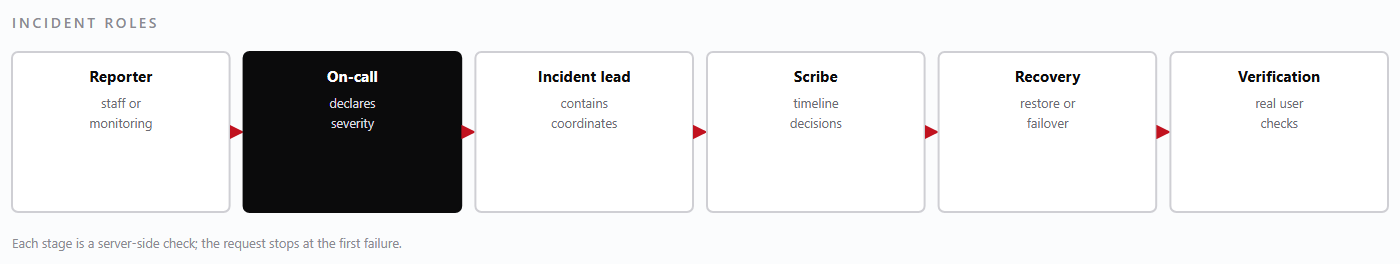
\includegraphics[width=\linewidth]{images/fig-21.png}
\caption{— Incident roles. In a small team one person may hold two roles, but the scribe role is never dropped.Figure 21}
\end{figure}
\begin{notebox}NoteThe scribe is the most valuable role in a long incident and the first one omitted. A timeline written during the event is worth more than a reconstruction afterwards.\end{notebox}
\textsc{\small\color{crimson}9.6 · Communication and review}\par\medskip
\section*{Communication plan and post-incident review}
\section{9.6 Communication plan}
9 · Disaster ManagementLoveLaundry — System Manual

\begin{center}\small
\begin{tabularx}{\linewidth}{|X|X|X|}
\hline
\rowcolor{lightgrey}
\textbf{Audience} & \textbf{Trigger} & \textbf{Channel and content} \\ \hline
Laundry owner & SEV1, SEV2 & Phone within 15 minutes: what is affected, what is being done, next update time \\ \hline
Laundry manager and supervisors & Any severity affecting trading & Direct message: workaround instructions and what to record on paper \\ \hline
Hotel clients & Their records or invoices are affected & Written notice from the laundry: what happened, what was corrected, what they should check \\ \hline
All staff & SEV1, or any change to procedure & Notice at next sign-in or shift briefing \\ \hline
Data protection contact & Personal data may have been accessed & Immediate written notice with the facts known at the time \\ \hline
\end{tabularx}
\end{center}
Communication during an incident is factual and time-bound. Say what is known, what is not known, and when the next update will come. Never speculate about cause or recovery time, and never blame a named individual — the review establishes cause, not the incident channel.

\section{9.7 Post-incident review}
Every SEV1 and SEV2 incident gets a written review within one business day. The review is blameless in method but specific in outcome: it must produce changes with owners and dates, not a narrative of what everyone did wrong.

\begin{center}\small
\begin{tabularx}{\linewidth}{|X|X|}
\hline
\rowcolor{lightgrey}
\textbf{Section} & \textbf{Content} \\ \hline
Timeline & Detection, declaration, containment, recovery, verification — with times \\ \hline
Impact & What was unavailable, for how long, and which records were affected \\ \hline
Cause & The technical cause and the contributing conditions that let it matter \\ \hline
What worked & Controls that did their job, so they are not removed in the next redesign \\ \hline
Actions & Specific changes, each with an owner and a due date \\ \hline
Verification & How the fix will be tested, and when the review is closed \\ \hline
\end{tabularx}
\end{center}
\begin{notebox}WarningAn action without an owner and a date is a wish. If a review produces more than five actions, it has produced none that will be done — choose the ones that change the outcome.\end{notebox}
\textsc{\small\color{crimson}9.8 · Incident severity matrix}\par\medskip
\section*{Incident severity matrix}
One table that decides who is called and how fast.

9 · Disaster ManagementLoveLaundry — System Manual

\begin{figure}[htbp]
\centering
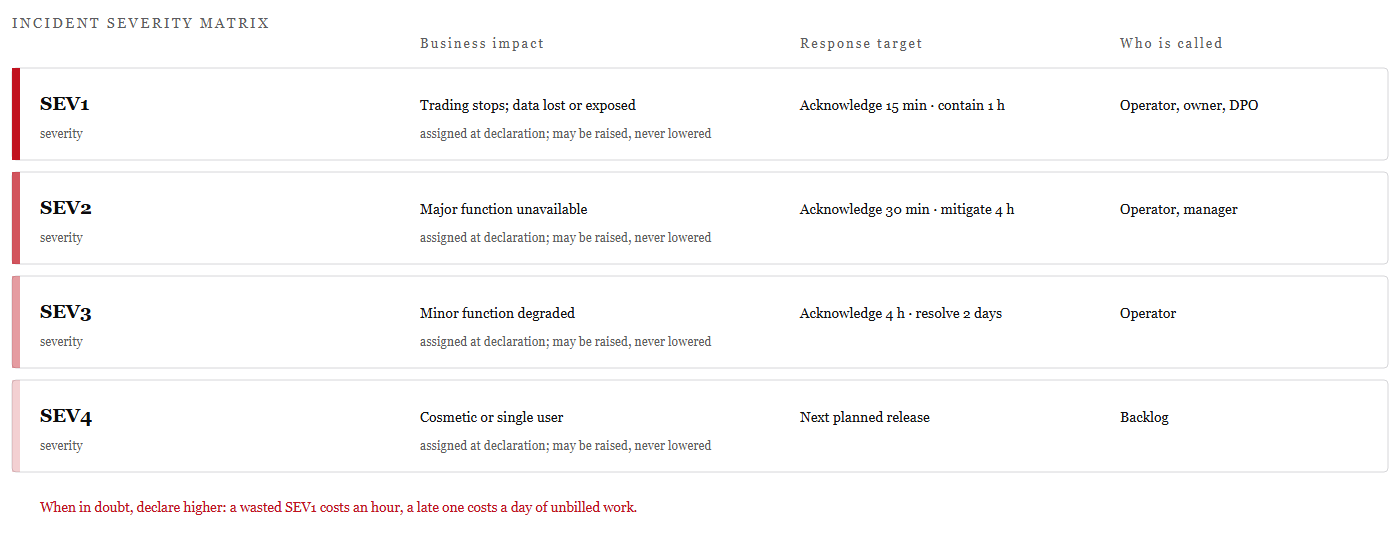
\includegraphics[width=\linewidth]{images/fig-22.png}
\caption{— Severity bands with response targets and the people they summon.Figure 22}
\end{figure}
Severity is assigned at declaration, from business impact rather than technical curiosity. A dull configuration error that stops billing is Sev1; an exotic defect in a report nobody reads is Sev3.

The matrix is read downwards, not upwards: start at the impact, then take the response target that belongs to it. The target is measured from declaration, not from the moment someone understands the cause.

\begin{notebox}RuleSeverity may be raised during an incident and is never lowered. Lowering it mid-incident invites people to stand down before the work is finished.\end{notebox}
\textsc{\small\color{crimson}Part Three · Backup and Recovery}\par\medskip
\chapter{Backup and Recovery}
\begin{quote}\itshape What is protected, how quickly it must come back, and how the restore is proved rather than assumed.\end{quote}
\section{10.1 What is backed up}
Backups exist to restore a business, not to archive a server. The inventory below therefore follows the three-database model: everything that cannot be rebuilt from source is backed up, and everything that can be rebuilt is not.

10 · Backup and RecoveryLoveLaundry — System Manual

\begin{center}\small
\begin{tabularx}{\linewidth}{|X|X|X|}
\hline
\rowcolor{lightgrey}
\textbf{Item} & \textbf{Method} & \textbf{Why it is backed up} \\ \hline
user\_db & Nightly logical dump plus continuous oplog & Identity and tenancy; without it nobody can sign in \\ \hline
Operations database & Nightly logical dump plus continuous oplog & Gate passes, deliveries, bills, linen history — the trading record \\ \hline
Accounting database & Nightly logical dump & Ledger and payroll; changes slowly, restored independently \\ \hline
Uploaded documents and printed artefacts & Object-storage versioning & Bill PDFs and attachments referenced by records \\ \hline
Configuration & Version-controlled environment templates, secrets in the key store & A host can be rebuilt only if its configuration is known \\ \hline
KEK and search-key escrow & Separate secure escrow, distinct access policy & Encrypted fields are unreadable without them \\ \hline
Audit log & Append-only log pipeline with extended retention & Needed for investigation after an incident \\ \hline
\end{tabularx}
\end{center}
\subsubsection*{What is deliberately not backed up}
Front-end bundles are rebuilt from the tagged commit, not backed up as files. Container images are rebuilt from the same commit. Temporary caches, session state and search indexes hold nothing that cannot be reconstructed. Backing these up would lengthen every restore without changing the outcome.

\begin{notebox}WarningA backup that has never been restored is a hypothesis. The drill in 10.7 exists because the most common backup failure is a backup that completes successfully and cannot be read.\end{notebox}
\textsc{\small\color{crimson}10.2 · RPO and RTO targets}\par\medskip
\section*{Recovery objectives}
Recovery point objective (RPO) is how much data the business can afford to lose. Recovery time objective (RTO) is how long it can afford to be without the function. Both are business statements that the technical design must meet — not measurements of what happens to be possible.

\begin{center}\small
\begin{tabularx}{\linewidth}{|X|X|X|X|}
\hline
\rowcolor{lightgrey}
\textbf{Component} & \textbf{RPO} & \textbf{RTO} & \textbf{Basis} \\ \hline
user\_db & 15 minutes & 1 hour & Oplog replay from the last dump; identity is a precondition for everything \\ \hline
Operations database & 15 minutes & 2 hours & Oplog replay; the trading record, largest restore \\ \hline
Accounting database & 24 hours & 4 hours & Daily dump is sufficient; restores independently \\ \hline
Object storage & 24 hours & 1 hour & Versioning; documents referenced by records \\ \hline
Application host & Not applicable & 2 hours & Rebuilt from configuration, no state \\ \hline
Full estate & 15 minutes & 4 hours & Sequential restore in dependency order \\ \hline
\end{tabularx}
\end{center}
10 · Backup and RecoveryLoveLaundry — System Manual

\begin{figure}[htbp]
\centering
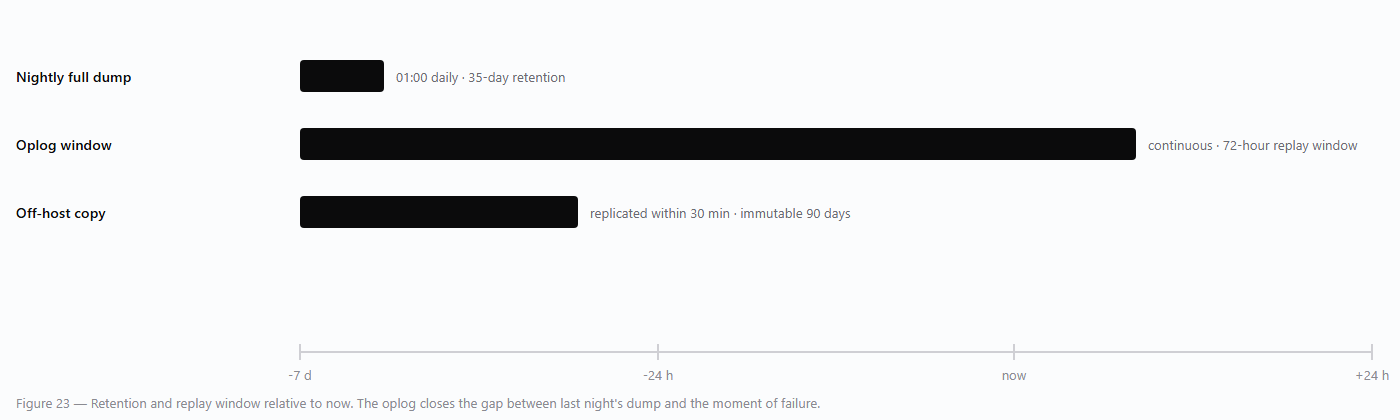
\includegraphics[width=\linewidth]{images/fig-23.png}
\caption{— Backup, retention and point-in-time recovery timeline.Figure 23}
\end{figure}
\begin{notebox}NoteThe 15-minute RPO depends on the oplog being intact. If the oplog is lost with the database, the achievable RPO becomes 24 hours, which is why the oplog is replicated off-host and monitored as a first-class backup artefact.\end{notebox}
\textsc{\small\color{crimson}10.3 · Backup schedule}\par\medskip
\section*{Backup schedule}
Backups run on a schedule, are copied off-host, and are verified by a job that reads them back. A backup job that reports success without a verification step is reporting that a file was written, not that it can be used.

\begin{center}\small
\begin{tabularx}{\linewidth}{|X|X|X|X|}
\hline
\rowcolor{lightgrey}
\textbf{Job} & \textbf{Frequency} & \textbf{Retention} & \textbf{Destination} \\ \hline
user\_db logical dump & Daily 01:00 & 35 daily, 12 monthly & Object storage, separate account \\ \hline
Operations dump & Daily 01:15 & 35 daily, 12 monthly & Object storage, separate account \\ \hline
Accounting dump & Daily 01:30 & 35 daily, 24 monthly & Object storage, separate account \\ \hline
Oplog archive & Continuous & 72 hours & Object storage, separate account \\ \hline
Configuration snapshot & On every deployment & Indefinite (version control) & Repository \\ \hline
Restore verification & Weekly & Latest verified copy recorded & Isolated environment \\ \hline
Full drill & Quarterly & Report retained 2 years & Isolated environment \\ \hline
\end{tabularx}
\end{center}
\subsubsection*{Ordering and overlap}
The three dumps are staggered so that they do not compete for disk or network, and so that a failure in one does not delay the others. The operations dump is the longest and runs second; the accounting dump is small and runs last. Every job writes a manifest containing the start time, end time, byte count, database name and checksum, which is what the verification job reads.

\subsubsection*{Monitoring the schedule}
10 · Backup and RecoveryLoveLaundry — System Manual

\begin{itemize}
\item A missed job raises an alert within 15 minutes of its expected completion.
\item A job that completes with a size more than 20 percent below its recent average is treated as suspect and alerted, not accepted.
\item Two consecutive verification failures are a Severity 2 incident, because the business is one failure away from having no usable backup.
\end{itemize}
\begin{notebox}WarningNever store the only backup copy on the host being backed up. Ransomware and disk failure both remove the backup and the data in one event.\end{notebox}
\textsc{\small\color{crimson}10.4 · Restore procedure}\par\medskip
\section*{Restore procedure}
Restore order is fixed: user\_db first, operations second, accounting third. Operations documents reference users and memberships; accounting references operational documents. Restoring out of order produces a database that looks complete and is internally inconsistent.

\subsubsection*{Procedure — restoring to a clean host}
\begin{enumerate}
\item Take the application out of service so that no writes occur during the restore. Announce the maintenance window.\textbf{Freeze.}
\item Build the host and install the database version recorded in the release notes. Do not restore into a different major version without a tested upgrade path.\textbf{Provision.}
\item Retrieve the chosen dump and its manifest from object storage. Verify the checksum against the manifest before use.\textbf{Fetch.}
\item Load the dump, then apply oplog entries up to the target time if point-in-time recovery is required.\textbf{Restore user\_db.}
\item Confirm that users, laundries and memberships are present and that a known administrator can authenticate.\textbf{Verify identity.}
\item Load the dump into the operations database and replay the oplog to the same target time.\textbf{Restore operations.}
\item Load the accounting dump, then reconcile its payment totals against the restored operations data.\textbf{Restore accounting.}
\item Confirm that a known encrypted field decrypts with the escrowed KEK. A restore with the wrong key is indistinguishable from data loss until someone opens a record.\textbf{Re-encrypt check.}
\item Bring services up in dependency order and run the smoke checks in 10.5.\textbf{Start services.}
\item Write the restore record: operator, dump identifiers, target time, duration, verification results.\textbf{Record.}
\end{enumerate}
\begin{notebox}WarningDo not restore over a live database in place. Restore into a fresh database, verify, then switch the connection string. An in-place restore that fails halfway leaves neither the old data nor the new.\end{notebox}
10 · Backup and RecoveryLoveLaundry — System Manual

\textsc{\small\color{crimson}10.5 · Verification and integrity checks}\par\medskip
\section*{Verification and integrity checks}
A restore is complete when the data is proved usable, not when the load command exits. The checks below run in order; the first failure stops the process and the restore is repeated from the previous step.

\begin{center}\small
\begin{tabularx}{\linewidth}{|X|X|X|}
\hline
\rowcolor{lightgrey}
\textbf{Check} & \textbf{Method} & \textbf{Pass condition} \\ \hline
Row counts & Count per collection against the manifest & Within the recorded tolerance; no empty core collection \\ \hline
Identity & Sign in as a known administrator & Sign-in succeeds and the tenant resolves \\ \hline
Tenancy & Request a record with a foreign tenant identifier & Returns not-found, never a record \\ \hline
Financial continuity & Sum bill totals, payments and balances & Balances equal totals less payments; no negative balance without a credit record \\ \hline
Referential integrity & Deliveries without a pass; bills without lines & Zero orphans \\ \hline
Linen consistency & Tags in a status with no corresponding event & Zero, or explained by the restore window \\ \hline
Encryption & Open a record with an encrypted field & Decrypts correctly; no key errors in the log \\ \hline
Recent activity & Open the last gate pass before the failure & Present with its deliveries intact \\ \hline
\end{tabularx}
\end{center}
\subsubsection*{Integrity queries worth keeping}
The financial check is the one that catches a partial restore most reliably, because a half-loaded set of payments still looks plausible in a list but cannot balance. The orphan check catches a restore that stopped between collections, which is exactly what happens when a restore is interrupted and resumed incorrectly.

\begin{verbatim}
// deliveries whose gate pass is absent
{"$lookup": {"from": "gate_passes", "localField": "gate_pass_id",
              "foreignField": "_id", "as": "gp"}},
{"$match": {"gp": []}}
\end{verbatim}
\begin{notebox}NoteKeep the verification queries in version control alongside the restore script. A check that exists only in someone's memory is not a control.\end{notebox}
\textsc{\small\color{crimson}10.6 · Point-in-time recovery}\par\medskip
\section*{Point-in-time recovery}
Point-in-time recovery (PITR) restores the database to a moment before a damaging change — a bad migration, a mistaken delete, a corrupting script. It combines the last full dump with oplog entries replayed up to, but not including, the harmful operation.

\subsubsection*{Procedure — recovering to a chosen moment}
10 · Backup and RecoveryLoveLaundry — System Manual

\begin{enumerate}
\item Identify the exact time of the harmful change from the audit log or the application log. Precision matters: replaying one minute too far re-applies the damage.
\item Confirm that the required window is inside the oplog retention. Outside it, only a full restore is possible.
\item Restore the most recent dump that precedes the target time into a fresh database.
\item Replay oplog entries from the dump's end time to the target time, excluding the harmful operation.
\item Verify with the checks in 10.5, then switch the connection string and restart the services.
\item Reconcile any work performed after the target time from paper or from client records, and enter it with its true date and a note explaining the gap.
\end{enumerate}
\begin{center}\small
\begin{tabularx}{\linewidth}{|X|X|X|}
\hline
\rowcolor{lightgrey}
\textbf{Situation} & \textbf{Target time} & \textbf{Rationale} \\ \hline
Accidental delete of one collection & Just before the delete & Minimises lost legitimate work \\ \hline
Bad migration altering many records & Just before the migration started & The migration's effects are the damage \\ \hline
Corruption of unknown origin & Last verified good state & Prefer a known-good point to a guessed one \\ \hline
Ransomware & Last backup before encryption began & Assume everything after is untrusted \\ \hline
\end{tabularx}
\end{center}
\begin{notebox}WarningReplaying to the exact second of a transaction boundary can leave a bill without its payment. Choose a recovery point at a quiet moment — end of day, or after a close — whenever the business can tolerate it.\end{notebox}
\textsc{\small\color{crimson}10.7 · Restore drill checklist}\par\medskip
\section*{Restore drill checklist}
The drill is performed quarterly against an isolated environment, using the same artefacts and the same procedure as a real recovery. It is timed, and the result is recorded — including the parts that failed.

\begin{center}\small
\begin{tabularx}{\linewidth}{|X|X|X|}
\hline
\rowcolor{lightgrey}
\textbf{Step} & \textbf{Check} & \textbf{Evidence recorded} \\ \hline
1 & Retrieve the latest dump and verify its checksum & Dump identifier, checksum, retrieval time \\ \hline
2 & Provision an isolated host with the recorded versions & Host identifier, versions \\ \hline
3 & Restore user\_db and authenticate as a known administrator & Time to first successful sign-in \\ \hline
4 & Restore operations and accounting databases & Time per database, total elapsed \\ \hline
5 & Run the integrity checks in 10.5 & Each check's result, including failures \\ \hline
6 & Decrypt a known sensitive field with the escrowed KEK & Field identifier, result \\ \hline
7 & Replay a five-minute oplog window & Target time, entries applied \\ \hline
8 & Run the smoke tests: pass, delivery, bill, hotel read & Screenshots or ids of created records \\ \hline
9 & Compare achieved RPO and RTO with the targets & Measured values against 10.2 \\ \hline
10 & Destroy the isolated environment & Destruction time, operator \\ \hline
\end{tabularx}
\end{center}
10 · Backup and RecoveryLoveLaundry — System Manual

\subsubsection*{What the drill must produce}
\begin{itemize}
\item A measured restore duration, compared with the RTO. A drill that is not timed does not test the objective.
\item A list of every step that required improvisation, because each is a gap in this chapter.
\item Confirmation that the KEK escrow works from a clean environment, not from the operator's workstation.
\item An updated procedure if any step was wrong. The manual is corrected the same week, not at the next review.
\end{itemize}
\begin{notebox}NoteRecord failures in the drill report. A clean report that everyone knows was helped along is worse than a failed drill that gets fixed.\end{notebox}
\textsc{\small\color{crimson}10.8 · Backup and recovery timeline}\par\medskip
\section*{Backup and recovery timeline}
Three overlapping protections, and the fifteen minutes that separates them.

\begin{figure}[htbp]
\centering
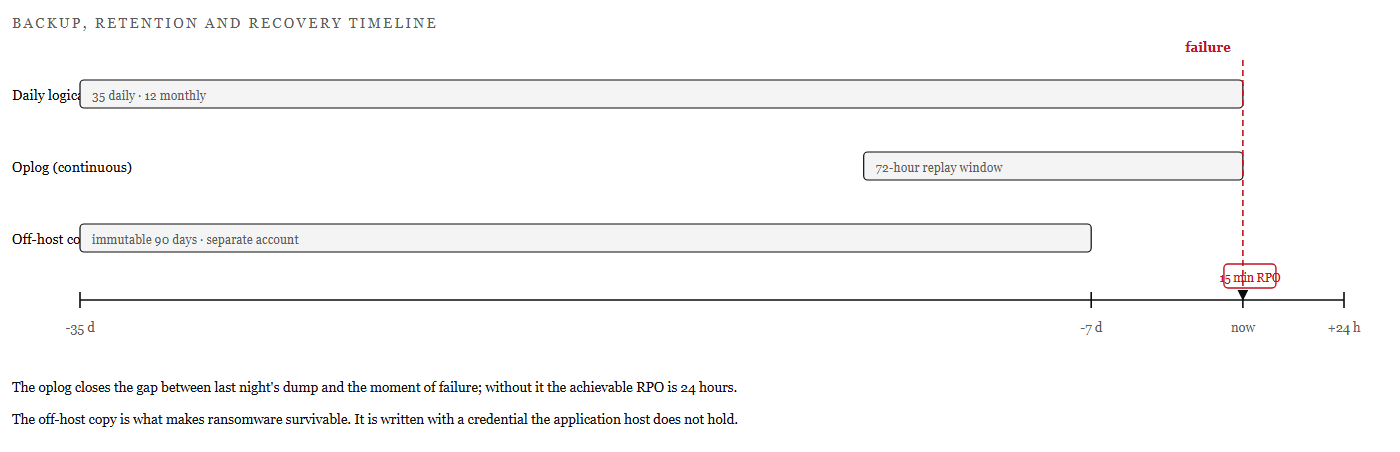
\includegraphics[width=\linewidth]{images/fig-24.png}
\caption{— Daily dumps, continuous oplog and the off-host copy, against the recovery-point target.Figure 24}
\end{figure}
The restore procedure itself begins on page 98, and the drill checklist on page 100. The timeline explains why the recovery-point target is fifteen minutes rather than a day. The nightly dump sets the floor, the oplog closes the gap to the moment of failure, and the off-host copy survives the loss of the host that wrote it.

Each layer answers a different failure. The dump answers corruption, the oplog answers a bad change made an hour ago, and the off-host copy answers the loss of the account in which everything else lives.

\begin{notebox}RuleThe oplog is a backup artefact, not a log to be pruned for space. If it is lost with the database, the achievable recovery point becomes the last dump.\end{notebox}
\textsc{\small\color{crimson}Part Three · Fail-Safes and Resilience}\par\medskip
\chapter{Fail-Safes and Resilience}
\begin{quote}\itshape How the platform behaves when something is missing, slow, or called twice.\end{quote}
\section{11.1 Fail-closed tenancy}
The platform's most important fail-safe is also its simplest: when the tenant cannot be established, nothing happens. There is no default tenant, no fallback to an unscoped query, and no “system” mode that skips the check. A request that cannot name its laundry is refused before it reaches any data.

\begin{center}\small
\begin{tabularx}{\linewidth}{|X|X|X|}
\hline
\rowcolor{lightgrey}
\textbf{Condition} & \textbf{Outcome} & \textbf{Why} \\ \hline
No token & 401 & Identity is unknown \\ \hline
Expired or badly signed token & 401 & Identity cannot be trusted \\ \hline
Client token on a staff route & 403 & No tenant claim exists to resolve \\ \hline
Staff token with no laundry\_id & 403 & Tenant context missing; fail closed \\ \hline
Membership removed since issue & 403 after the account is disabled & Capabilities are snapshot at sign-in \\ \hline
Foreign identifier in a path & 404 & Indistinguishable from a non-existent record \\ \hline
\end{tabularx}
\end{center}
\subsubsection*{Why fail closed rather than fail open}
11 · Fail-Safes and ResilienceLoveLaundry — System Manual

A fail-open design answers a missing tenant with “all tenants”, which turns a configuration mistake into a data breach. Fail-closed turns the same mistake into an outage — visible, recoverable, and confined to the person who caused it. For a multi-tenant system holding other businesses' commercial records, an outage is the cheaper failure every time.

\begin{notebox}NoteThe same principle applies to capabilities: an unknown or missing capability is treated as absent, never as permitted. New routes must declare a capability or they cannot be reached at all.\end{notebox}
\textsc{\small\color{crimson}11.2 · Idempotency and concurrency}\par\medskip
\section*{Idempotency and optimistic concurrency}
Two failures cause most duplicate records in operational systems: a retried request that actually succeeded, and two users editing the same document. The platform addresses both explicitly rather than hoping they are rare.

\subsubsection*{Idempotency keys}
Every write that creates money or possession — bill, payment, delivery, gate pass — accepts an idempotency key generated by the client. The server records the key with the result. A retry with the same key returns the original result instead of creating a second record, whether the first attempt succeeded, failed, or is still in progress.

\begin{figure}[htbp]
\centering
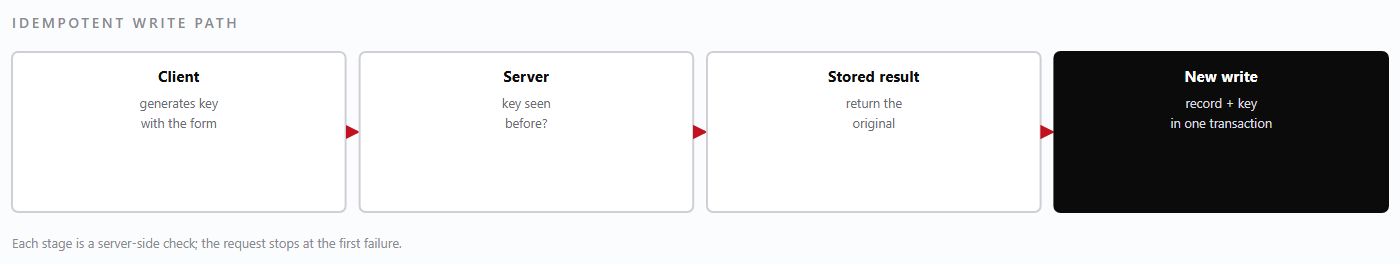
\includegraphics[width=\linewidth]{images/fig-25.png}
\caption{— Idempotent write path. The key and the record are committed together, so a crash cannot leave one without the other.Figure 25}
\end{figure}
\subsubsection*{Optimistic concurrency}
Documents that can be edited carry a version. An update must state the version it read; if the stored version has moved, the write is rejected with a conflict instead of silently overwriting a colleague's change. The user is shown both versions and chooses — which is slower by one interaction and correct by construction.

\begin{center}\small
\begin{tabularx}{\linewidth}{|X|X|X|}
\hline
\rowcolor{lightgrey}
\textbf{Situation} & \textbf{Response} & \textbf{User experience} \\ \hline
Same document, sequential edits & Accepted; version increments & Normal editing \\ \hline
Same document, simultaneous edits & Second write rejected with 409 & Message shows the other change; reload and retry \\ \hline
Retry after timeout & Idempotency key returns the original result & The action appears to have succeeded, because it did \\ \hline
Duplicate key without a stored result & Write rejected as in-progress & The user is asked to wait rather than double-submit \\ \hline
\end{tabularx}
\end{center}
11 · Fail-Safes and ResilienceLoveLaundry — System Manual

\begin{notebox}NoteIdempotency keys are generated per form submission, not per user action. Reopening a bill and paying again is a new intent and gets a new key, which is why the confirmation step matters.\end{notebox}
\textsc{\small\color{crimson}11.3 · Atomic bill and payment transitions}\par\medskip
\section*{Atomic bill and payment transitions}
Money movements are the one place where a partial write is unacceptable. A payment that reduces a balance without being recorded, or a bill that is issued without its lines, is worse than a failed request because it is invisible until reconciliation.

\subsubsection*{What must happen together}
\begin{center}\small
\begin{tabularx}{\linewidth}{|X|X|}
\hline
\rowcolor{lightgrey}
\textbf{Operation} & \textbf{Writes that must commit together} \\ \hline
Issue bill & Bill document with lines and totals; sequence number; client balance \\ \hline
Post payment & Payment record; bill balance; receipt reference; audit entry \\ \hline
Reverse payment & Reversal record referencing the original; restored balance; audit entry \\ \hline
Record delivery & Delivery document; pass line delivered quantities; pass status \\ \hline
Close day & Day-close record with totals; frozen date marker; audit entry \\ \hline
\end{tabularx}
\end{center}
MongoDB multi-document transactions make each of these a single unit. The platform uses them only where the invariant spans documents — a transaction has a cost, and paying it on a read is waste. Where a single document holds the whole invariant, an atomic update on that document is sufficient and cheaper.

\subsubsection*{Why the bill is not edited after issue}
An issued bill is a document the client may already hold. Editing it would change the meaning of a record that exists outside the platform, and no transaction can undo that. Corrections are therefore new documents — credit notes, adjustments, reversals — each referencing the original, so the history remains a sequence of facts rather than a current opinion.

\begin{notebox}WarningNever “fix” a balance by writing the field directly. A balance is derived from records; writing it creates a number that no document supports, and the next reconciliation will fail with no explanation.\end{notebox}
\textsc{\small\color{crimson}11.4 · Offline cache, retries and circuit breaking}\par\medskip
\section*{Offline cache, retries and circuit breaking}
A laundry is a physical place with unreliable connectivity: a basement linen room, a counter by a steel door, a driver's phone. The front ends are built to stay useful for reading when the network is poor, and to refuse to pretend when it is absent.

\subsubsection*{Offline cache behaviour}
11 · Fail-Safes and ResilienceLoveLaundry — System Manual

\begin{itemize}
\item Lists and detail views may be served from the last successful response, clearly marked as cached with the time it was fetched.\textbf{Cached reads, never cached writes.}
\item The platform does not store a write locally and replay it later with an invented timestamp. A scan recorded at 14:05 must not enter the system as 09:12.\textbf{No queued writes.}
\item A cached view says when it was last updated; a user who sees “as of 09:12” knows to phone rather than assume.\textbf{Explicit staleness.}
\item Cached business data does not survive a session on a shared terminal.\textbf{Sign-out clears the cache.}
\end{itemize}
\subsubsection*{Retries and queues}
Reads retry automatically with exponential backoff and jitter, up to a small limit. Writes retry only when the request is idempotent, and always with the same key, so that a retry cannot create a second bill. Where a write triggers a cross-service side effect — mirroring a payment into accounting — the platform writes a durable outbox record in the same transaction as the business write and processes it asynchronously. If the accounting service is down, the payment still posts; the outbox retries until it succeeds, and the discrepancy is visible rather than lost.

\subsubsection*{Circuit breaking}
When a dependency fails repeatedly, the caller stops calling it for a short period and fails fast instead of queueing requests that will time out. This protects the healthy services from thread and connection exhaustion caused by one sick dependency. The breaker closes automatically after a successful probe, and its state is exposed as a health detail so that an operator can see “degraded because accounting is down” rather than a generic error.

\begin{notebox}NoteFail fast is a feature. A request that waits thirty seconds and then fails is worse for the user and for the system than one that fails in fifty milliseconds and says why.\end{notebox}
\textsc{\small\color{crimson}11.5 · Degraded-mode matrix}\par\medskip
\section*{Degraded-mode matrix}
The matrix states what still works when a component is unavailable. It is written from the operator's point of view: during an incident, the question is never “which service is down?” but “can we still take in laundry and bill for it?”

11 · Fail-Safes and ResilienceLoveLaundry — System Manual

\begin{center}\small
\begin{tabularx}{\linewidth}{|X|X|X|X|}
\hline
\rowcolor{lightgrey}
\textbf{If this is down…} & \textbf{Still works} & \textbf{Stops} & \textbf{Workaround} \\ \hline
user-service & Nothing authenticated & Everything & Restore identity first — it is the precondition for all else \\ \hline
bill\_service & Sign-in; quotations; accounting reads & Passes, deliveries, bills, linen, shop, hotel portal & Paper records with times; enter after recovery \\ \hline
laundry-management & All operational work & Accounting posting, payroll, expense entry & Outbox queues payments; reconcile after recovery \\ \hline
quotation-service & All operational and financial work & Quotation drafting and AI chat & Price manually and record once service returns \\ \hline
worker-service & All operational work & Worker lists and attendance & Record attendance on paper for the shift \\ \hline
MongoDB primary & Reads served by secondary, briefly & All writes & Wait for election; do not force a primary \\ \hline
Object storage & All application functions & Backups, document download & Alert immediately; local backup copy retained \\ \hline
Reverse proxy & Nothing from outside & All client access & Restore proxy config; services remain healthy \\ \hline
\end{tabularx}
\end{center}
\subsubsection*{Reading the matrix in an incident}
The first column that is empty tells you the severity. If sign-in is down, everything is down and the incident is SEV1 regardless of the technical cause. If only accounting is down, the laundry can trade all day and the incident is SEV2 with an outbox reconciliation afterwards.

\begin{notebox}WarningA workaround that bypasses a control is not a workaround. Paper records are acceptable; entering a bill twice “to be safe”, or marking a card payment as cash, is not.\end{notebox}
\textsc{\small\color{crimson}11.6 · Guard rails against double billing}\par\medskip
\section*{Guard rails against double billing}
Double billing is the failure clients notice fastest and forgive slowest. The platform defends against it at four layers, so that no single mistake — human or technical — can produce a duplicate charge.

\begin{center}\small
\begin{tabularx}{\linewidth}{|X|X|X|}
\hline
\rowcolor{lightgrey}
\textbf{Layer} & \textbf{Control} & \textbf{What it prevents} \\ \hline
Data & A delivery line can belong to only one bill & The same delivered quantity being billed twice \\ \hline
Transaction & Bill issue and delivery marking commit together & A bill issued without consuming its deliveries \\ \hline
Request & Idempotency key on bill creation & A retried issue creating a second bill \\ \hline
Process & Day-close review of unbilled deliveries and duplicate totals & Anything the first three layers missed \\ \hline
\end{tabularx}
\end{center}
11 · Fail-Safes and ResilienceLoveLaundry — System Manual

\subsubsection*{How a duplicate would still be caught}
\begin{enumerate}
\item The bill list shows consecutive bills for the same client with identical totals and periods — flagged in the day-close review.
\item A delivery already consumed by a bill is not offered when raising the next bill, so the second attempt produces an empty selection rather than a duplicate.
\item A client statement shows both invoices with their numbers; the hotel portal makes the duplicate visible to the client the same day.
\item The audit trail records who issued each bill and when, which distinguishes a duplicate from a legitimate re-issue.
\end{enumerate}
\subsubsection*{Correcting a duplicate}
Void the duplicate with a reason and re-check the client's balance. Do not delete it: a voided bill keeps its number and remains visible, which is what allows the client's copy and the platform's record to agree. If the duplicate has been paid, reverse the payment and void the bill, then issue a credit note if the client's money must be returned through accounting.

\begin{notebox}NoteEvery guard rail here is also a test in the bill\_service suite. The controls and the tests are maintained together, because a guard rail that is not tested is a comment.\end{notebox}
\textsc{\small\color{crimson}11.7 · Guard layers against double billing}\par\medskip
\section*{Guard layers against double billing}
Four independent defences, so that no single mistake produces a duplicate charge.

\begin{figure}[htbp]
\centering
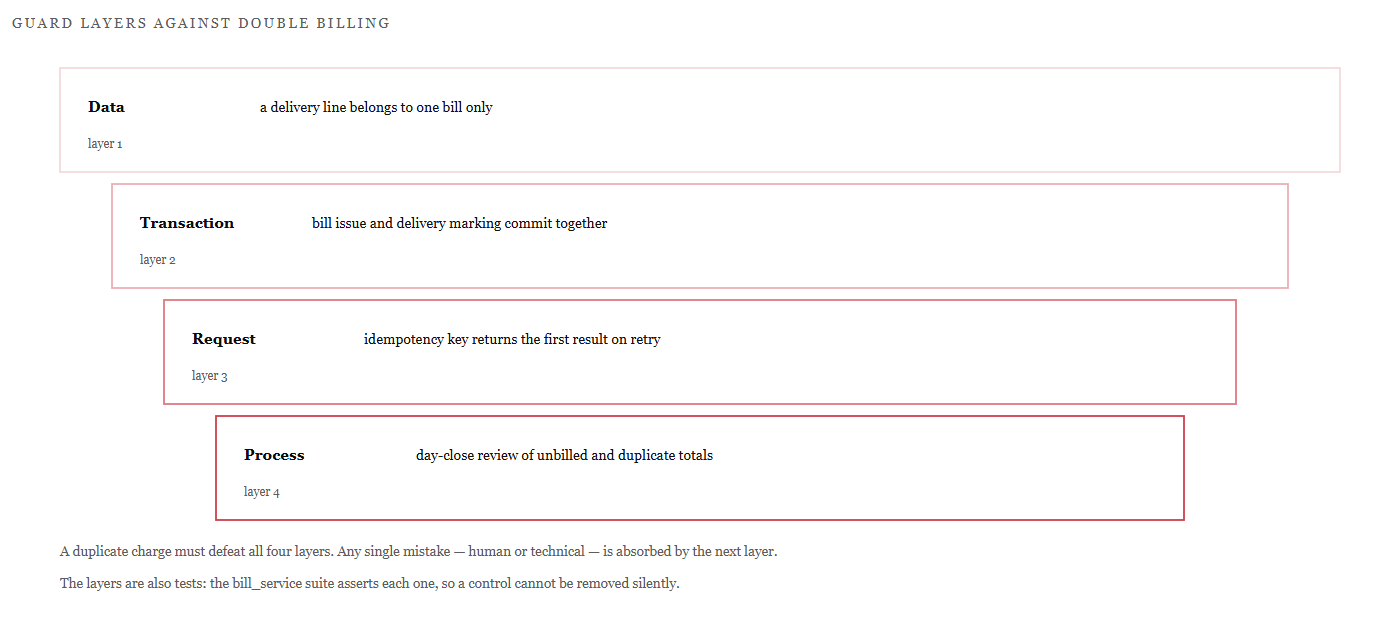
\includegraphics[width=\linewidth]{images/fig-26.png}
\caption{— Layered defences against double billing, from the data model to the day-close review.Figure 26}
\end{figure}
11 · Fail-Safes and ResilienceLoveLaundry — System Manual

A duplicate charge is the failure clients notice fastest and forgive slowest, so the platform does not rely on one control. The data model prevents a delivered line from belonging to two bills; the transaction prevents a bill from existing without consuming its lines; the idempotency key prevents a retry from creating a second document.

The fourth layer is human and deliberately boring: the day-close review looks for consecutive bills with identical totals. It exists to catch the combinations the first three layers cannot foresee.

\begin{notebox}RuleEach layer is also a test in the bill\_service suite. A control that is not asserted is a comment, and comments do not survive refactoring.\end{notebox}
\part{Assurance and Reference}
\textsc{\small\color{crimson}Part Four · Testing and Quality Assurance}\par\medskip
\chapter{Testing and Quality Assurance}
\begin{quote}\itshape What is tested, what the suites actually report, and what remains unproven.\end{quote}
\section{12.1 Test strategy}
The strategy is a pyramid, and it is deliberately bottom-heavy. Most behaviour is verified by fast service-level tests that exercise real handlers against a test database; a smaller number of integration tests cover cross-service contracts; and the top of the pyramid — where confidence is most expensive — is thin. That is a deliberate trade: a browser-driven suite for four applications would be slow, brittle, and rarely run.

12 · Testing and Quality AssuranceLoveLaundry — System Manual

\begin{figure}[htbp]
\centering
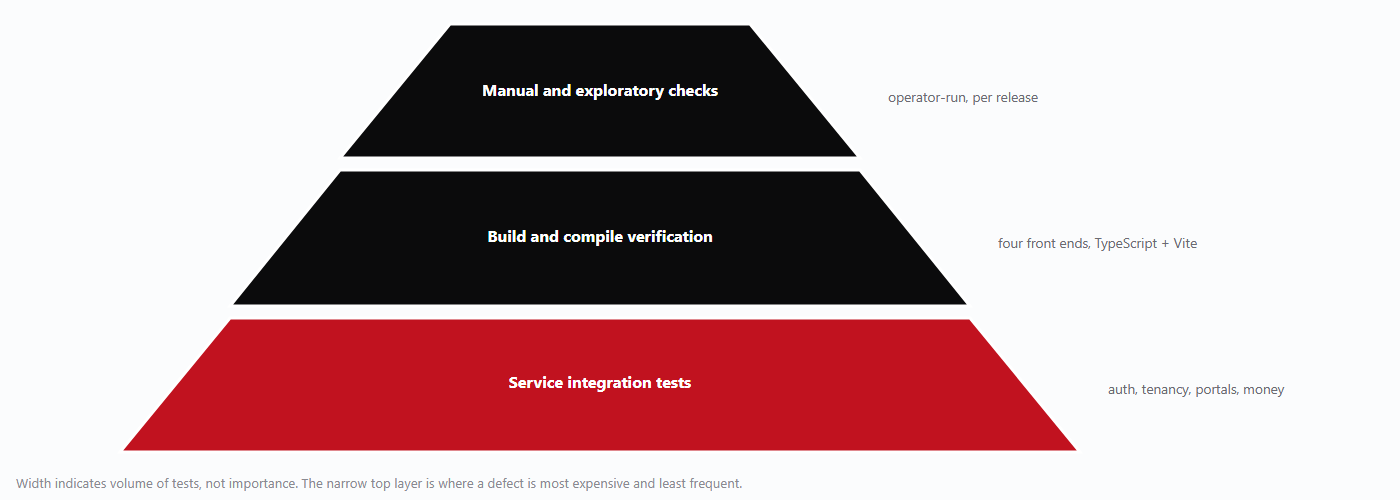
\includegraphics[width=\linewidth]{images/fig-27.png}
\caption{— Test strategy pyramid: broad service-level coverage, thin top layer.Figure 27}
\end{figure}
\begin{center}\small
\begin{tabularx}{\linewidth}{|X|X|X|}
\hline
\rowcolor{lightgrey}
\textbf{Layer} & \textbf{Exercises} & \textbf{Runs in} \\ \hline
Unit & Pure functions: totals, tax, status transitions, token parsing & Seconds, no database \\ \hline
Service & HTTP handlers with authentication and a test database & The service's own suite \\ \hline
Integration & Cross-service flows: login → pass → delivery → bill; client portal scope & bill\_service and user-service suites \\ \hline
Build & TypeScript compilation and Vite production build for all four apps & CI or local release check \\ \hline
Manual & Exploratory checks of new screens and print layouts & Before each release \\ \hline
\end{tabularx}
\end{center}
\begin{notebox}NoteTests run against a real MongoDB instance, not a mock. Tenancy and transaction behaviour are precisely the things a mock cannot reproduce, and they are the properties most worth testing.\end{notebox}
\textsc{\small\color{crimson}12.2 · Measured results}\par\medskip
\section*{Measured results}
The figures below are measured from the suites as they stand. They are reported as counts of passing tests, not as coverage percentages, because a coverage number would say more about the size of the codebase than about whether the important behaviour is verified.

12 · Testing and Quality AssuranceLoveLaundry — System Manual

\begin{center}\small
\begin{tabularx}{\linewidth}{|X|X|X|}
\hline
\rowcolor{lightgrey}
\textbf{Suite} & \textbf{Result} & \textbf{Notes} \\ \hline
user-service & 68 tests passing & Authentication, users, laundries, memberships, client accounts, token claims \\ \hline
bill\_service & 380 passing, 2 skipped & Operational core: passes, deliveries, bills, shop bills, linen lifecycle, returns, matrix, dispatch, day close, dashboard, client portal \\ \hline
— of which client portal & 13 tests & Included in the 380; covers scope filtering, summary, passes, deliveries, bills \\ \hline
shop-app & Compiles and builds & TypeScript compilation and Vite production build succeed \\ \hline
hotel-app & Compiles and builds & TypeScript compilation and Vite production build succeed \\ \hline
linen-room-app & Compiles and builds & TypeScript compilation and Vite production build succeed \\ \hline
quotations-ui & Builds & Existing application; build verified as part of the release check \\ \hline
\end{tabularx}
\end{center}
\subsubsection*{How to read these numbers}
A passing suite means the behaviour it asserts still holds. It does not mean the product is defect-free, and the two skipped tests are skipped deliberately rather than hidden: they cover paths that require an external dependency not configured in the current environment. Chapter 12.3 states the gaps plainly.

\subsubsection*{What is deliberately not claimed}
\begin{itemize}
\item No coverage percentage is quoted, because line coverage would be misleading for a codebase with a large amount of declarative schema.
\item No performance figures are quoted, because no load test has been run.
\item No browser-level pass rate is quoted, because there is no browser-driven end-to-end suite.
\end{itemize}
\begin{notebox}NoteReporting a measured 380 rather than a rounded “over 400” is itself part of the quality claim. The manual should not be more confident than the suites.\end{notebox}
\textsc{\small\color{crimson}12.3 · Coverage and gaps}\par\medskip
\section*{What is covered and what is not}
The table below is the honest boundary. It should be read before any release decision, and it should be updated whenever a gap is closed.

12 · Testing and Quality AssuranceLoveLaundry — System Manual

\begin{center}\small
\begin{tabularx}{\linewidth}{|X|X|X|}
\hline
\rowcolor{lightgrey}
\textbf{Area} & \textbf{Covered} & \textbf{Gap} \\ \hline
Authentication and tokens & Sign-in, wrong password, expired token, token kind, claims & — \\ \hline
Tenancy isolation & Missing tenant, foreign identifier, client token on staff route & Cross-tenant aggregation edge cases are covered by a single test \\ \hline
Gate passes and deliveries & Creation, status, partial delivery, over-delivery rejection & Bulk import paths are not exercised \\ \hline
Bills and payments & Issue, immutability, payment posting, reversal, balances & Concurrent payment posting is tested at the unit level only \\ \hline
Shop bills & Creation, tender, day close totals & Refund approval workflow is lightly covered \\ \hline
Linen lifecycle & All ten actions, invalid transitions, discrepancy records & Scanner hardware behaviour is simulated, not real \\ \hline
Hotel client portal & Scope filtering, summary, passes, deliveries, bills & PDF rendering of invoices is not asserted \\ \hline
Front-end applications & TypeScript compilation and production build & No rendered-DOM or interaction tests \\ \hline
\end{tabularx}
\end{center}
\begin{figure}[htbp]
\centering
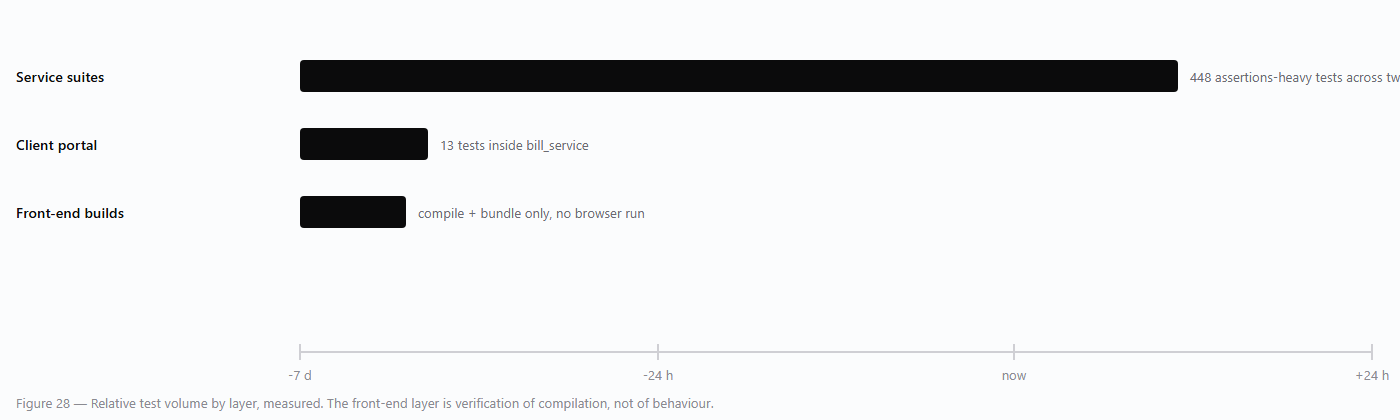
\includegraphics[width=\linewidth]{images/fig-28.png}
\caption{— Measured coverage by layer.Figure 28}
\end{figure}
\begin{notebox}WarningThere is no browser-driven end-to-end suite and no load testing. A regression that only appears when a real browser renders a real form will not be caught by these suites; it must be caught by the manual release check.\end{notebox}
\textsc{\small\color{crimson}12.4 · Running the suites}\par\medskip
\section*{Running the suites}
Each service has its own virtual environment and its own suite. Running them is a local operation and requires a reachable MongoDB instance; the tests create and drop their own database.

\subsubsection*{Service suites}
12 · Testing and Quality AssuranceLoveLaundry — System Manual

\begin{verbatim}
cd user-service
python -m venv .venv
.venv\Scripts\activate
pip install -r requirements.txt
python -m pytest -q

cd ..\bill_service
python -m pytest -q
\end{verbatim}
The expected results are the ones stated in 12.2: 68 passing for user-service, and 380 passing with 2 skipped for bill\_service. A different count means the environment differs from the one those figures were measured in — check the Python version and the installed dependencies before treating it as a regression.

\subsubsection*{Front-end builds}
\begin{verbatim}
cd shop-app
npm ci
npm run build

# repeat for hotel-app, linen-room-app, quotations-ui
\end{verbatim}
A successful build is the release gate for the front ends: TypeScript must compile with no errors and Vite must emit a bundle. Warnings are reviewed but do not block a release unless they indicate an unused secret or a missing environment variable.

\begin{center}\small
\begin{tabularx}{\linewidth}{|X|X|X|}
\hline
\rowcolor{lightgrey}
\textbf{Symptom} & \textbf{Cause} & \textbf{Action} \\ \hline
Collection error naming a missing module & Dependency absent from the local virtualenv & Install the dependency, or accept the documented gap in 12.5 \\ \hline
Database connection refused & No local MongoDB, or wrong URI & Start MongoDB and set the test URI \\ \hline
Tests pass individually but fail together & Shared state between tests & Report as a defect; do not reorder tests to hide it \\ \hline
Build fails on a missing VITE\_ variable & Environment file absent & Copy the example env file and fill the values \\ \hline
\end{tabularx}
\end{center}
\textsc{\small\color{crimson}12.5 · Known environment limitations}\par\medskip
\section*{Known environment limitations}
One suite cannot be collected in the local virtual environment.  imports , which is not installed there. This is an environment gap, not a product defect: the middleware it exercises is covered indirectly by the authentication and tenancy tests that do run, and the module is expected to collect once the dependency is present.\texttt{tests/test\_security\_middleware.py}\texttt{httpx2}

12 · Testing and Quality AssuranceLoveLaundry — System Manual

\begin{center}\small
\begin{tabularx}{\linewidth}{|X|X|X|}
\hline
\rowcolor{lightgrey}
\textbf{Limitation} & \textbf{Effect} & \textbf{Status} \\ \hline
missing in the local virtualenv\texttt{httpx2} & cannot be collected\texttt{tests/test\_security\_middleware.py} & Environment gap; install the dependency to include it \\ \hline
No browser-driven end-to-end suite & Rendered behaviour is verified manually & Accepted gap; manual release check required \\ \hline
No load or soak testing & Throughput and behaviour under sustained load are unknown & Accepted gap; monitor in production \\ \hline
2 skipped bill\_service tests & Paths requiring an unconfigured external dependency are unexercised & Deliberate skip; documented here \\ \hline
Scanner hardware not simulated & Scan timing and wedge-mode behaviour are not asserted & Accepted gap; station test at deployment \\ \hline
\end{tabularx}
\end{center}
\subsubsection*{Why these are stated rather than hidden}
A manual that lists only what works is a sales document. The value of this chapter is that a new maintainer can see exactly where confidence ends — and can decide, with the owner, whether a gap matters for the next release. The gaps above are known, bounded and owned; none of them is a surprise waiting to be discovered during an incident.

\begin{notebox}NoteClosing the  gap requires only adding the dependency to the test requirements. It is listed as a limitation rather than fixed here because this manual reports the environment as measured, not as it could be.\texttt{httpx2}\end{notebox}
\textsc{\small\color{crimson}Part Four · Operations Runbook and Monitoring}\par\medskip
\chapter{Operations Runbook and Monitoring}
\begin{quote}\itshape The routine that keeps the platform observable, and the first five minutes of the incidents that interrupt it.\end{quote}
\section{13.1 Health checks}
Each service exposes a health endpoint that answers two questions separately: is the process alive, and can it reach what it depends on? A single combined check is worse than useless, because it cannot distinguish a dead service from a healthy service with a dead database.

\begin{center}\small
\begin{tabularx}{\linewidth}{|X|X|X|}
\hline
\rowcolor{lightgrey}
\textbf{Probe} & \textbf{Checks} & \textbf{Used by} \\ \hline
Liveness & Process responds; no dependency access & Supervisor restart policy \\ \hline
Readiness & Database reachable; key material loaded & Reverse proxy rotation \\ \hline
Deep health & Database round-trip, key version, outbox backlog & Monitoring, every minute \\ \hline
Auth probe & A known test account can sign in (staging only) & Release verification \\ \hline
\end{tabularx}
\end{center}
13 · Operations Runbook and MonitoringLoveLaundry — System Manual

\begin{figure}[htbp]
\centering
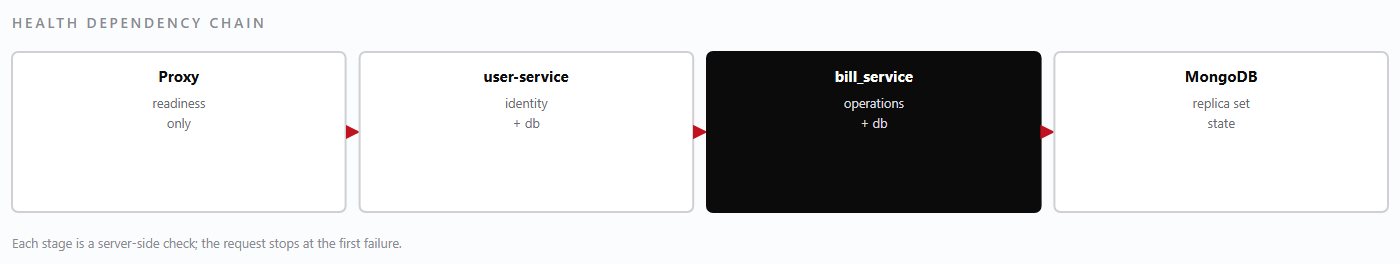
\includegraphics[width=\linewidth]{images/fig-29.png}
\caption{— Health dependency chain. The proxy routes only to services whose readiness probe passes.Figure 29}
\end{figure}
Health output is JSON with a status per dependency, so that a monitoring system can alert on the specific dependency rather than on “service unhealthy”. The outbox backlog is included because a service that is healthy but cannot drain its queue is failing slowly and silently.

\begin{notebox}NoteNever use a deep health check as a liveness probe. A database blip would then restart healthy services, turning a short dependency failure into a restart storm.\end{notebox}
\textsc{\small\color{crimson}13.2 · Logs}\par\medskip
\section*{Logs}
Logs are structured JSON, one event per line, written to stdout and collected by the log pipeline. They are designed to answer “who did what, to which record, in which tenant, and did it work?” without a debugger.

\begin{center}\small
\begin{tabularx}{\linewidth}{|X|X|}
\hline
\rowcolor{lightgrey}
\textbf{Field} & \textbf{Content} \\ \hline
time & ISO-8601 timestamp with offset \\ \hline
level & info, warning, error \\ \hline
service & user-service, bill\_service, and so on \\ \hline
request\_id & Correlates every log line from one request, including cross-service calls \\ \hline
user\_id / role & Actor, when authenticated \\ \hline
laundry\_id & Tenant, when resolved — never a tenant guessed from the payload \\ \hline
action & Route or operation name \\ \hline
target & Record identifier, when applicable \\ \hline
outcome & Status code or result class \\ \hline
duration\_ms & Handler duration \\ \hline
\end{tabularx}
\end{center}
\subsubsection*{What is never logged}
\begin{itemize}
\item Passwords, in any form, including on failed sign-in.
\item Bearer tokens or signing keys.
\item Full request bodies for authentication and payment routes.
\item Personal data beyond what an audit entry requires.
\end{itemize}
13 · Operations Runbook and MonitoringLoveLaundry — System Manual

\subsubsection*{Retention and access}
Application logs are retained for 30 days at full detail and 12 months at reduced detail. Audit entries are retained for seven years and are append-only. Access to logs is restricted to the platform operator; a laundry administrator may be given a filtered extract for their own tenant when investigating a dispute, but never a cross-tenant view.

\begin{notebox}WarningA stack trace that includes a connection string is a credential leak. The logging configuration redacts known secret patterns, but new code must not log configuration objects wholesale.\end{notebox}
\textsc{\small\color{crimson}13.3 · Alerts and first response}\par\medskip
\section*{Alerts and first response}
An alert is only useful if the first action is obvious. Each alert below names the likely cause and the first thing to check, so that the person woken at night does not begin with an investigation.

\begin{center}\small
\begin{tabularx}{\linewidth}{|X|X|X|}
\hline
\rowcolor{lightgrey}
\textbf{Alert} & \textbf{Likely cause} & \textbf{First response} \\ \hline
Sign-in failure rate above baseline & Credential stuffing, or a broken key rotation & Check the failure reason distribution; block the source if it is external \\ \hline
5xx rate above baseline on bill\_service & Database unreachable, or a bad release & Check readiness and the most recent deployment \\ \hline
Backup job missed & Scheduler stopped, or storage credential expired & Run the job manually; verify the credential \\ \hline
Backup size drop > 20\% & Partial dump or empty database & Treat as failed; do not rotate retention until explained \\ \hline
Disk usage above 80\% & Log growth or oplog retention & Prune logs, verify retention policy, plan capacity \\ \hline
Oplog window below 24 hours & Write volume outpacing oplog size & Increase oplog size before the RPO degrades \\ \hline
Outbox backlog growing & Accounting service unavailable & Check the dependency; the queue drains on recovery \\ \hline
Certificate expiring in 14 days & Renewal failed & Renew manually; verify the proxy reload \\ \hline
Repeated 403 on one account & Role removed, or a client token used on a staff route & Confirm the account type and membership \\ \hline
\end{tabularx}
\end{center}
\subsubsection*{Escalation discipline}
Acknowledge, then act. An alert acknowledged and forgotten is worse than one ignored, because it hides the problem from everyone else. If the first response does not resolve the alert within its target, escalate the severity rather than extending the window quietly.

\begin{notebox}NoteAlert fatigue is a design defect. If an alert fires routinely without action, either the threshold is wrong or the underlying problem should be fixed; leaving it in place trains people to ignore the one that matters.\end{notebox}
13 · Operations Runbook and MonitoringLoveLaundry — System Manual

\textsc{\small\color{crimson}13.4 · Routine maintenance calendar}\par\medskip
\section*{Routine maintenance calendar}
Maintenance is scheduled so that it never competes with a day close or a Monday collection. The calendar is deliberately boring: the same tasks, at the same cadence, with the same owner.

\begin{center}\small
\begin{tabularx}{\linewidth}{|X|X|X|}
\hline
\rowcolor{lightgrey}
\textbf{Cadence} & \textbf{Task} & \textbf{Owner} \\ \hline
Daily & Verify the overnight backups completed and their sizes are normal & Platform operator \\ \hline
Daily & Review the error log for new patterns & Platform operator \\ \hline
Weekly & Run the restore verification job against the latest dump & Platform operator \\ \hline
Weekly & Review refunds, voids and discounts by user & Laundry manager \\ \hline
Monthly & Apply operating-system and dependency security updates & Platform operator \\ \hline
Monthly & Review disk, oplog window and database growth & Platform operator \\ \hline
Quarterly & Full restore drill with timing (10.7) & Platform operator \\ \hline
Quarterly & Review the risk register and incident actions & Owner and operator \\ \hline
Annually & Rotate the search key with a planned backfill & Platform operator \\ \hline
Annually & Review roles, memberships and dormant accounts & Laundry administrator \\ \hline
\end{tabularx}
\end{center}
\begin{figure}[htbp]
\centering
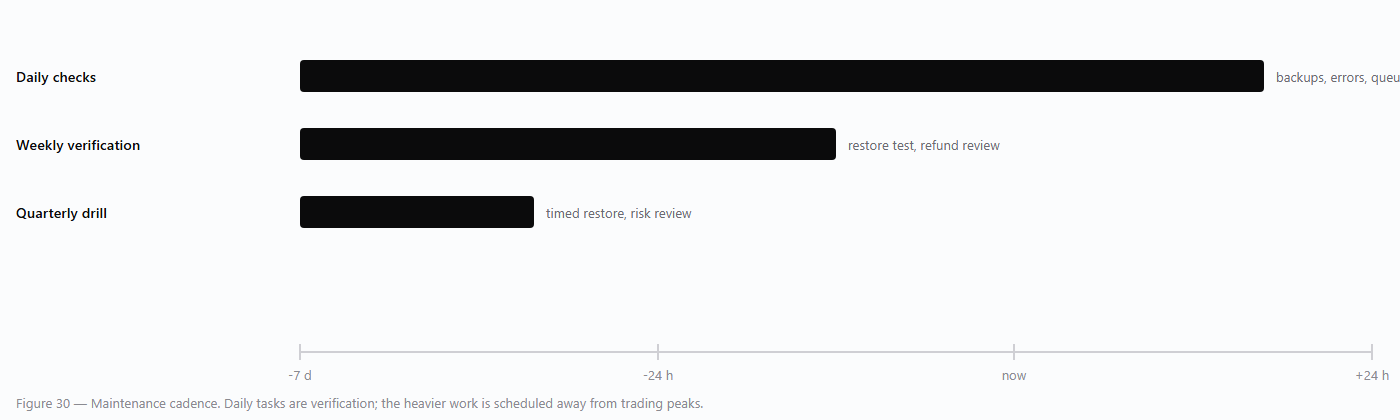
\includegraphics[width=\linewidth]{images/fig-30.png}
\caption{— Maintenance calendar by cadence.Figure 30}
\end{figure}
\begin{notebox}WarningNever apply security updates to the database host during trading hours without a tested rollback. A patched database that will not start is an outage with a maintenance window's worth of warning wasted.\end{notebox}
\textsc{\small\color{crimson}13.5 · Alert and escalation flow}\par\medskip
\section*{Alert and escalation flow}
From signal to review, with the loop that raises severity when nobody answers.

13 · Operations Runbook and MonitoringLoveLaundry — System Manual

\begin{figure}[htbp]
\centering
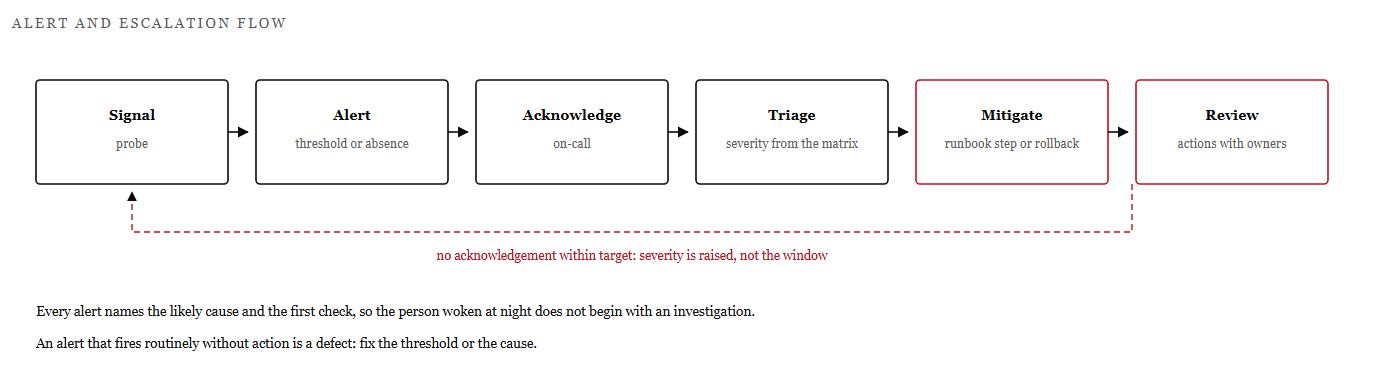
\includegraphics[width=\linewidth]{images/fig-31.png}
\caption{— Alert lifecycle and the escalation loop when acknowledgement does not happen within target.Figure 31}
\end{figure}
An alert is only useful if the first action is obvious, so every alert in the catalogue names a likely cause and the first thing to check. The flow above is the path from a signal to a written action, and it is deliberately short.

The loop at the top is the part that is usually missing: if nobody acknowledges within the target, severity is raised rather than the window quietly extended.

\begin{notebox}RuleAn alert that fires routinely without action is a design defect. Either the threshold is wrong or the cause should be fixed; leaving it trains people to ignore the one that matters.\end{notebox}
\textsc{\small\color{crimson}Part Four · Appendices}\par\medskip
\chapter{Appendices}
\begin{quote}\itshape Reference tables, matrices and enumerations: endpoints, roles, statuses, vocabulary and revision history.\end{quote}
AppendicesLoveLaundry — System Manual

\begin{center}\small
\begin{tabularx}{\linewidth}{|X|X|X|X|}
\hline
\rowcolor{lightgrey}
\textbf{Method} & \textbf{Path} & \textbf{Purpose} & \textbf{Auth} \\ \hline
POST & /auth/login & Staff sign-in; returns a 24-hour staff token & None \\ \hline
POST & /auth/refresh & Issue a fresh token for a valid session & Staff token \\ \hline
GET & /users & List users in the tenant & ADMIN \\ \hline
POST & /users & Create a user & ADMIN \\ \hline
PATCH & /users/\{id\} & Update display name or status & ADMIN \\ \hline
GET & /laundries & List laundries & PLATFORM\_ADMIN \\ \hline
POST & /laundries & Create a laundry (tenant) & PLATFORM\_ADMIN \\ \hline
GET & /laundries/\{laundry\_id\}/members & List memberships for the tenant & ADMIN \\ \hline
POST & /laundries/\{laundry\_id\}/members & Grant a role to a user & ADMIN \\ \hline
DELETE & /laundries/\{laundry\_id\}/members/\{id\} & Remove a user's access & ADMIN \\ \hline
\end{tabularx}
\end{center}
\begin{center}\small
\begin{tabularx}{\linewidth}{|X|X|X|X|}
\hline
\rowcolor{lightgrey}
\textbf{Method} & \textbf{Path} & \textbf{Purpose} & \textbf{Auth} \\ \hline
POST & /client/auth/login & Hotel client sign-in; 12-hour client token & None \\ \hline
GET & /client/auth/status & Current client account state & Client token \\ \hline
GET & /clients & List client accounts for the tenant & ADMIN, MANAGER \\ \hline
POST & /clients & Create a client account bound to one client\_name & ADMIN \\ \hline
PATCH & /clients/\{id\}/status & Enable or disable a client account & ADMIN \\ \hline
\end{tabularx}
\end{center}
\begin{notebox}NoteStaff routes reject client tokens because the tenant dependency cannot resolve  from a client token. Client routes reject staff tokens for the mirror-image reason: there is no .\texttt{laundry\_id}\texttt{client\_scope}\end{notebox}
\textsc{\small\color{crimson}Appendix A · API reference}\par\medskip
\section*{API reference — bill\_service}
AppendicesLoveLaundry — System Manual

\begin{center}\small
\begin{tabularx}{\linewidth}{|X|X|X|}
\hline
\rowcolor{lightgrey}
\textbf{Method} & \textbf{Path} & \textbf{Purpose} \\ \hline
GET & /gatepasses & List passes for the tenant, filtered by status and date \\ \hline
POST & /gatepasses & Create a pass with item lines \\ \hline
GET & /gatepasses/\{id\} & Pass detail with lines and delivery history \\ \hline
PATCH & /gatepasses/\{id\} & Amend a pass (manager or above) \\ \hline
POST & /gatepasses/\{id\}/cancel & Cancel with a reason; the number is retained \\ \hline
GET & /deliveries & List deliveries \\ \hline
POST & /deliveries & Record a delivery against pass lines \\ \hline
GET & /deliveries/\{id\} & Delivery detail and receiver \\ \hline
POST & /deliveries/\{id\}/reverse & Reverse a delivery with a reason \\ \hline
GET & /bills & List bills with status and balance \\ \hline
POST & /bills & Raise a bill from unbilled deliveries \\ \hline
GET & /bills/\{id\} & Bill detail with lines and payments \\ \hline
POST & /bills/\{id\}/payments & Post a payment against the bill \\ \hline
POST & /payments/\{payment\_id\}/reverse & Reverse a posted payment \\ \hline
\end{tabularx}
\end{center}
\begin{center}\small
\begin{tabularx}{\linewidth}{|X|X|X|}
\hline
\rowcolor{lightgrey}
\textbf{Method} & \textbf{Path} & \textbf{Purpose} \\ \hline
GET & /shop-bills & List counter sales for a business date \\ \hline
POST & /shop-bills & Create a shop bill \\ \hline
POST & /shop-bills/\{id\}/record-payment & Complete payment and issue the receipt \\ \hline
POST & /shop-bills/\{id\}/void & Void before payment, with a reason \\ \hline
POST & /shop-bills/\{id\}/refund & Refund a paid bill; requires approval \\ \hline
GET & /monthly/\{kind\}/\{client\}/\{yy\}/\{mm\} & Client-by-day quantities and values \\ \hline
GET & /bills/unbilled-gatepasses & Deliveries not yet on a bill \\ \hline
POST & /day-close & Close the business date \\ \hline
GET & /day-close/\{date\} & Close record for a date \\ \hline
GET & /dashboard & Operational tiles for the tenant \\ \hline
\end{tabularx}
\end{center}
\textsc{\small\color{crimson}Appendix A · API reference}\par\medskip
\section*{API reference — linen, portal and supporting services}
AppendicesLoveLaundry — System Manual

\begin{center}\small
\begin{tabularx}{\linewidth}{|X|X|X|}
\hline
\rowcolor{lightgrey}
\textbf{Method} & \textbf{Path} & \textbf{Purpose} \\ \hline
GET & /linens & List tags by status, client or item type \\ \hline
POST & /linens/\{doc\_id\}/scan & Submit a scan event for a tag \\ \hline
POST & /linens/\{tag\}/action & Apply a lifecycle action to a tag \\ \hline
GET & /linens/\{tag\}/history & Full event history for a tag \\ \hline
POST & /linens/\{tag\}/retire & Retire an item (supervisor only) \\ \hline
GET & /linens & Counts by status, type and client \\ \hline
GET & /linens/stats/summary & Open and closed discrepancies \\ \hline
\end{tabularx}
\end{center}
\begin{center}\small
\begin{tabularx}{\linewidth}{|X|X|X|}
\hline
\rowcolor{lightgrey}
\textbf{Method} & \textbf{Path} & \textbf{Purpose} \\ \hline
GET & /client-portal/summary & Passes in progress, items returned, outstanding balance \\ \hline
GET & /client-portal/gatepasses & Passes scoped to the client\_name in client\_scope \\ \hline
GET & /client-portal/deliveries & Deliveries scoped to the client\_name \\ \hline
GET & /client-portal/bills & Invoices for this property \\ \hline
GET & /client-portal/bills/\{id\} & Invoice detail, scoped by both keys \\ \hline
\end{tabularx}
\end{center}
\begin{center}\small
\begin{tabularx}{\linewidth}{|X|X|X|}
\hline
\rowcolor{lightgrey}
\textbf{Service} & \textbf{Responsibility} & \textbf{Front end} \\ \hline
quotation-service & Quotations, line pricing, AI chat & quotations-ui \\ \hline
worker-service & Worker records and attendance & quotations-ui \\ \hline
laundry-management & Customers, transactions, payments, expenses, salary, employees, items & quotations-ui \\ \hline
love-ai & Drafting and summarised answers over permitted data & quotations-ui \\ \hline
\end{tabularx}
\end{center}
\begin{notebox}NoteEvery client-portal query filters on both  and . A request that supplies only an invoice identifier returns the invoice only if both keys match; otherwise it is indistinguishable from a non-existent record.\texttt{laundry\_id}\texttt{client\_name}\end{notebox}
\textsc{\small\color{crimson}Appendix B}\par\medskip
\section*{Role and capability matrix}
The matrix is the authoritative statement of which role holds which capability.  means granted; a blank cell means refused, and a refused capability is refused by the server regardless of what the interface shows.●

AppendicesLoveLaundry — System Manual

\begin{center}\small
\begin{tabularx}{\linewidth}{|X|X|X|X|X|X|X|X|X|}
\hline
\rowcolor{lightgrey}
\textbf{Capability} & \textbf{ADMIN} & \textbf{PLATFORM\_ADMIN} & \textbf{MANAGER} & \textbf{STAFF} & \textbf{LINEN\_SUP.} & \textbf{HOUSEKEEPER} & \textbf{HOTEL\_ADMIN} & \textbf{HOTEL\_MGR} \\ \hline
gatepass:read & ● & ● & ● & ● & ● &  & ●¹ & ●¹ \\ \hline
gatepass:write & ● & ● & ● & ● &  &  &  &  \\ \hline
delivery:read & ● & ● & ● & ● & ● &  & ●¹ & ●¹ \\ \hline
delivery:write & ● & ● & ● & ● &  &  &  &  \\ \hline
bill:read & ● & ● & ● & ● &  &  & ●¹ & ●¹ \\ \hline
bill:write & ● & ● & ● & ● &  &  &  &  \\ \hline
payment:read & ● & ● & ● &  &  &  &  &  \\ \hline
payment:write & ● & ● & ● &  &  &  &  &  \\ \hline
linen:read & ● & ● & ● & ● & ● & ● &  &  \\ \hline
linen:scan & ● & ● & ● &  & ● & ● &  &  \\ \hline
linen:write & ● & ● & ● &  & ● &  &  &  \\ \hline
dashboard:read & ● & ● & ● & ● & ● & ● &  &  \\ \hline
report:read & ● & ● & ● &  &  &  &  &  \\ \hline
user management & ● & ● &  &  &  &  &  &  \\ \hline
tenant creation &  & ● &  &  &  &  &  &  \\ \hline
\end{tabularx}
\end{center}
¹ Hotel roles do not hold staff capabilities. Their access to gate passes, deliveries and bills is granted by  endpoints that check , not by the capability list. The marks are shown here to make the read-only equivalence visible; the mechanism is different, and deliberately so.\texttt{/client-portal}\texttt{client\_scope}

\begin{notebox}NotePLATFORM\_ADMIN is a superset of ADMIN, but only across tenants. It still cannot read a hotel client's records without a client session, because the portal scope is a separate dimension.\end{notebox}
\textsc{\small\color{crimson}Appendix C}\par\medskip
\section*{Status enumerations}
Statuses are stored as fixed strings. They are listed here because they appear in exports, reports and hotel-facing documents, and parsed by external tools that must not invent new values.

AppendicesLoveLaundry — System Manual

\begin{center}\small
\begin{tabularx}{\linewidth}{|X|X|X|}
\hline
\rowcolor{lightgrey}
\textbf{Document} & \textbf{Values} & \textbf{Notes} \\ \hline
Gate pass & received, in\_wash, ready, delivered, closed, cancelled & Cancelled passes retain their number \\ \hline
Delivery & recorded, reversed & Reversal is a new record referencing the original \\ \hline
Bill & draft, issued, part\_paid, paid, void & Issued bills are immutable \\ \hline
Payment & posted, reversed & Reversal never deletes the original \\ \hline
Shop bill & draft, open, paid, refunded, void & Separate numbering from laundry bills \\ \hline
Quotation & draft, sent, accepted, declined, expired & Conversion creates work, not a bill \\ \hline
Linen tag & collected, received, in\_wash, washed, pressed, ready, delivered, missing, damaged, retired & Ten lifecycle states, forward transitions only \\ \hline
Discrepancy & open, resolved, written\_off & Resolution requires a supervisor \\ \hline
Client account & active, disabled & Disabled blocks new sign-ins \\ \hline
User & active, disabled & Membership removal is separate from disabling \\ \hline
\end{tabularx}
\end{center}
\subsubsection*{Why fixed strings}
Free-text statuses make reports unreliable, because every spelling becomes a category. Fixed enumerations mean the monthly matrix, the dashboard and the hotel portal all count the same thing. When a new status is genuinely required, it is added to the enumeration, to the transition rules and to the tests in the same change.

\begin{notebox}WarningNever write a status that is not in this table. A value the platform does not recognise will disappear from every filtered view while remaining in the database, which is the hardest kind of missing record to find.\end{notebox}
\textsc{\small\color{crimson}Appendix D}\par\medskip
\section*{Glossary}
Terms as they are used in this manual and in the interface. Where a term has a narrower meaning here than in general use, the narrower meaning applies.

AppendicesLoveLaundry — System Manual

\begin{center}\small
\begin{tabularx}{\linewidth}{|X|X|}
\hline
\rowcolor{lightgrey}
\textbf{Term} & \textbf{Definition} \\ \hline
Audit entry & An append-only record of a security-relevant action: actor, tenant, action, target, outcome. \\ \hline
Capability & A named permission such as bill:write, carried in the token and checked per route. \\ \hline
Client account & A hotel login stored in client\_accounts; scoped to one laundry and one client\_name. \\ \hline
client\_name & The string identifying a hotel on operational documents. Not an entity, not a tenant. \\ \hline
client\_scope & The claim object on a client token containing laundry\_id and client\_name. \\ \hline
Day close & The act of freezing a business date's totals and recording who closed it. \\ \hline
DEK & Data encryption key: a per-document key used with AES-256-GCM. \\ \hline
Delivery & The record of returning finished goods against a gate pass. \\ \hline
Discrepancy & A recorded mismatch in quantity, condition or status. \\ \hline
Gate pass & The document recording goods received from a client and the promise to return them. \\ \hline
Idempotency key & A client-generated key that makes a retried write return the original result. \\ \hline
KEK & Key-encryption key: wraps DEKs and is held outside the database. \\ \hline
Membership & The link between a user and a laundry, carrying a role. \\ \hline
Monthly matrix & A client-by-day grid of quantities and values derived from passes and deliveries. \\ \hline
Outbox & A durable record of a side effect to be retried until it succeeds. \\ \hline
RPO / RTO & Recovery point objective (acceptable data loss) and recovery time objective (acceptable downtime). \\ \hline
Search token & An HMAC-SHA256 value enabling equality search over encrypted fields. \\ \hline
Tenant & A laundry; identified by laundry\_id on every business document. \\ \hline
token\_kind & A claim distinguishing staff tokens from client tokens. \\ \hline
\end{tabularx}
\end{center}
\textsc{\small\color{crimson}Appendix E}\par\medskip
\section*{Revision history and conventions}
\begin{center}\small
\begin{tabularx}{\linewidth}{|X|X|X|X|}
\hline
\rowcolor{lightgrey}
\textbf{Version} & \textbf{Date} & \textbf{Author} & \textbf{Change} \\ \hline
0.1 & Sep 2026 & R. D. Siriwardhana & Outline and architecture notes; not issued \\ \hline
0.9 & Oct 2026 & R. D. Siriwardhana & Draft for internal review: chapters 1–8 \\ \hline
1.0 & 24 Oct 2026 & R. D. Siriwardhana & First complete issue: 105 pages, all chapters and appendices \\ \hline
\end{tabularx}
\end{center}
\subsection*{Document conventions}
AppendicesLoveLaundry — System Manual

\begin{center}\small
\begin{tabularx}{\linewidth}{|X|X|}
\hline
\rowcolor{lightgrey}
\textbf{Convention} & \textbf{Meaning} \\ \hline
Numbered procedure & Steps to be followed in order; each step is an action on the interface \\ \hline
Bold interface label & A control, field or screen name as it appears in the application \\ \hline
Monospace & Field name, endpoint, environment variable, status value or code \\ \hline
Note callout (navy) & Behaviour that is correct but easy to misread \\ \hline
Warning callout (accent) & An action that can lose data, expose it, or break a control \\ \hline
Figure n.m / Table n.m & Numbered by chapter; referenced in text by number \\ \hline
Page footer & Document title and page number on every page, including the cover \\ \hline
\end{tabularx}
\end{center}
\subsection*{Maintenance of this manual}
The manual is reviewed at every minor release and after every Severity 1 or 2 incident. A change to the platform that alters a procedure, an endpoint, a status value or a control requires a corresponding change here in the same release — a manual that lags the software is worse than no manual, because it is trusted.

\begin{notebox}NoteCorrections are recorded as new revisions rather than silent edits. The revision table is the record of what changed and when, and it is the first thing a new maintainer should read.\end{notebox}
\textsc{\small\color{crimson}Appendix F}\par\medskip
\section*{Index}
Page references are to the printed page numbers in the footer.

AppendicesLoveLaundry — System Manual

\begin{notebox}NoteBold page numbers in a printed index conventionally denote the principal treatment; this index gives a single page per term to keep the reference unambiguous.\end{notebox}
\textsc{\small\color{crimson}Appendix E · Registration}\par\medskip
\chapter{Registration and Enrolment}
\begin{quote}\itshape Who creates an account, what it is bound to, and how the two sides stay apart.\end{quote}
\subsection*{E.1 The three identities}
Every account belongs to one laundry, the business that does the washing. Staff accounts belong to the laundry itself and carry a membership. Client accounts belong to a laundry and to a customer name: the hotel or the shop. That pair is the isolation boundary, which is why a client session never receives a staff claim.

A hotel account is created with  HOTEL and a role of HOTEL\_ADMIN or HOTEL\_MANAGER. A shop account uses SHOP with SHOP\_ADMIN or SHOP\_STAFF. The same login may exist at several laundries, and each is a separate account row, so switching laundries changes what a session may read rather than widening it.\texttt{client\_type}

The first account of any hotel or shop is created by a laundry administrator. After that the customer’s own administrator can add colleagues on the same side, and only on the same side.

Appendix E · RegistrationLoveLaundry — System Manual

\subsection*{E.2 Who may create whom}
\begin{center}\small
\begin{tabularx}{\linewidth}{|X|X|X|X|X|X|}
\hline
\rowcolor{lightgrey}
\textbf{Action} & \textbf{Laundry admin} & \textbf{Hotel admin} & \textbf{Hotel staff} & \textbf{Shop admin} & \textbf{Shop staff} \\ \hline
Create a hotel or shop & yes & no & no & no & no \\ \hline
Create another administrator & yes & no & no & no & no \\ \hline
Add own staff & yes & yes & no & yes & no \\ \hline
Read own records & n/a & yes & yes & yes & yes \\ \hline
Raise a shop order & n/a & no & no & yes & yes \\ \hline
Confirm receipt & staff API & no & no & no & no \\ \hline
\end{tabularx}
\end{center}
Two rules keep the table true. The laundry and customer name of a new staff account are taken from the caller’s token, never from the request, so an administrator cannot enrol staff into somebody else’s hotel. And staff creation accepts only the non-administrator role of the same side, so the endpoint cannot mint a peer administrator.

Creating an administrator therefore always requires the laundry, which is also the party able to suspend the account afterwards.

Appendix E · RegistrationLoveLaundry — System Manual

\subsection*{E.3 Registering a hotel}
The laundry administrator posts the hotel’s first account. That customer name becomes the hotel’s identity on every gate pass, delivery and bill, so one spelling must be used everywhere: records are matched on it exactly.

with the client type, the role, the customer name, a login and a password. The laundry comes from the caller’s token, not the body.\textbf{Request.}\texttt{POST /clients}

The account without its password. A duplicate login inside the same laundry returns 409; a role that does not belong to the chosen client type returns 400.\textbf{Response.}

The administrator then signs in at  with the client type set. If the same login exists at more than one laundry the reply is 409 listing them, and the call is repeated with an explicit laundry.\texttt{POST /client/auth/login}

Appendix E · RegistrationLoveLaundry — System Manual

\subsection*{E.4 Registering a shop and its staff}
The shop flow is identical with one substitution:  is SHOP, the first account is SHOP\_ADMIN, and colleagues are SHOP\_STAFF. Endpoints, isolation and the 409 rules are unchanged.\texttt{client\_type}

Once the shop administrator is signed in, adding a colleague is  with a login, a name and a password. The role defaults to SHOP\_STAFF and any other value is refused.  lists everyone under that shop and nobody from another.\texttt{POST /client/staff}\texttt{GET /client/staff}

Appendix E · RegistrationLoveLaundry — System Manual

\subsection*{E.5 Sessions across several laundries}
A login registered at two laundries signs in once and then chooses. Without an explicit laundry the login is ambiguous, and the server refuses to guess: it returns 409 with the list. Once the choice is made, the token carries exactly that laundry.

\begin{center}\small
\begin{tabularx}{\linewidth}{|X|X|}
\hline
\rowcolor{lightgrey}
\textbf{Call} & \textbf{Purpose} \\ \hline
\texttt{POST /client/auth/login} & Sign in; 409 lists the laundries when ambiguous \\ \hline
\texttt{GET /client/auth/laundries} & Every laundry this login may enter, on its own side \\ \hline
\texttt{POST /client/auth/switch} & Re-issue the token for another of those laundries \\ \hline
\texttt{POST /client/auth/refresh} & New expiry, claims re-read from the database \\ \hline
\texttt{PATCH /clients/\{id\}/status} & Laundry admin suspends or archives an account \\ \hline
\end{tabularx}
\end{center}
Switching does not extend a session’s reach. The old token keeps its original scope and the new one carries a different single scope. A suspension takes effect at the next refresh or sign-in, so revocation is bounded by the token lifetime rather than immediate.

Appendix E · RegistrationLoveLaundry — System Manual

\subsection*{E.6 Failures worth recognising}
\begin{center}\small
\begin{tabularx}{\linewidth}{|X|X|X|}
\hline
\rowcolor{lightgrey}
\textbf{Status} & \textbf{Meaning} & \textbf{What to do} \\ \hline
409 & That login already exists in this laundry & Choose another login, or suspend the old account \\ \hline
409 & Sign-in is ambiguous across laundries & Repeat the call with an explicit laundry \\ \hline
403 & Token belongs to the other side, or lacks the role & Use the correct app and the correct role \\ \hline
400 & Role does not belong to the chosen client type & Hotel roles with HOTEL, shop roles with SHOP \\ \hline
404 & The record exists but not for this account & Check the laundry and the customer name \\ \hline
\end{tabularx}
\end{center}
\subsection*{E.7 Enrolment checklist}
Confirm the laundry exists. Fix the customer name spelling before the first account, because later records match it exactly. Create the administrator, sign in as that administrator, add staff, then suspend any placeholder account. Finally sign in as a staff member and confirm the screens show only that customer’s records.

Enrolment is complete when a staff account can sign in, see its own hotel or shop, and is refused by every endpoint belonging to the other side.

\end{document}
